\documentclass[
    oneside,
    10pt,
    language=italian,
    a4paper
]{notes}
    % My packages
    % \usepackage{boxedthm}
    \usepackage{numerical}
    \usepackage{algebra}
    \usepackage{analysis}
    \usepackage{nicematrix}
    \usepackage{minted}
    
\usemintedstyle{manni}
\setminted{
    % bgcolor=lightgray,
    fontsize=\small,
    breaklines=true,
    % escapeinside=||,
    mathescape=true,
    frame=single
}

\setcounter{MaxMatrixCols}{20}

\usetikzlibrary{external}
\tikzexternalize[prefix=figures/]
\tcbsetforeverylayer{shield externalize}

\let\oldtilde\tilde
\renewcommand{\tilde}[1]{\widetilde{#1}}

\makeatletter
\DeclareDocumentCommand{\Mat}{m}{
    \Mat@Args{#1}
}
\DeclareDocumentCommand{\Mat@Args}{ >{\SplitArgument{2}{,}}m }{\Mat@Aux#1}
\DeclareDocumentCommand{\Mat@Aux}{mmm}{
    {#1}^{#2 \times #3}
}
\makeatother

\newcommand{\smallvdots}{\vphantom{\int^0}\smash[t]{\vdots}}

\begin{document}

\author{Luca De Paulis}
\title{Calcolo Numerico}
\maketitle

\frontmatter{}
\tableofcontents

\mainmatter{}

\chapter{Aritmetica di macchina}
\section{Rappresentazione dei numeri di macchina}
\label{sez:machine_nums}

Il primo problema da risolvere quando si vuole fare analisi numerica è scegliere un metodo per rappresentare i numeri reali su una macchina. Infatti un generico numero reale ha potenzialmente una scrittura decimale infinita, dunque essendo le risorse disponibili in una macchina \emph{finite} dobbiamo trovare un modo di approssimarlo. 

\subsection{Virgola fissa}
Il primo metodo è il metodo \strong{a virgola fissa}: in questo metodo si rappresentano tutti i numeri nella loro forma decimale normale e si considerano esattamente $k$ cifre dopo la virgola.

Questo metodo è molto semplice e ci consente di fare operazioni elementari (come le somme o i prodotti) immediatamente ("in colonna"), tuttavia ha anche degli svantaggi evidenti, come \begin{itemize}
    \item il range dei numeri rappresentabili su $n$ cifre/bit è piccolo;
    \item siccome il numero di bit dedicato ai numeri dopo la virgola è basso, la precisione è molto bassa e assolutamente non adeguata ad applicazioni di analisi numerica.
\end{itemize}
Per questo è stata inventata la rappresentazione in virgola mobile.

\subsection{Virgola mobile}
Innanzitutto dobbiamo trovare un modo standard per rappresentare un qualsiasi numero reale. Per far ciò ci viene in aiuto il seguente teorema.

\begin{theorem}
    {Teorema di rappresentazione in base}
    {rapp_base}
    Sia $x \in \R$, $x \neq 0$ e sia $\beta \geq 2$ una base di rappresentazione. 
    
    Allora esistono e sono univocamente determinati un \strong{esponente} $p \in \Z$ e una successione di \strong{cifre} $\seqn[\big]{d_i}_{i \in \N}$ (con $d_i \in \Z$ per ogni $i$) per cui vale che
    \begin{enumerate}[(i)]
        \item $d_1 \neq 0$;
        \item $0 \leq d_i \leq \beta - 1$ per ogni $i$;
        \item la successione $d$ non è definitivamente uguale a $\beta - 1$, ovvero per ogni $k > 0$ esiste un $j \geq k$ tale che $d_j \neq \beta - 1$;
        \item si ha che \[
            x = \sgn{x} \cdot \beta^p \cdot \parens*{\sum_{i=1}^\infty d_i\beta^{-i}}.
        \] 
    \end{enumerate}
\end{theorem}

La rappresentazione di $x$ nella forma data dal \Cref{th:rapp_base} si dice \strong{rappresentazione normalizzata in virgola mobile}.

\begin{example}
    Consideriamo ad esempio il numero reale $123$. Per il \Cref{th:rapp_base} possiamo esprimere $123$ come \[
        123 = +10^3 \cdot (0.123) = + 10^3 \cdot (1 \cdot 10\inv + 2 \cdot 10^{-2} + 3 \cdot 10^{-3}).
    \] Questa rappresentazione è l'unica possibile se imponiamo che $d_1$ sia diverso da $0$ e che le cifre della rappresentazione siano tutte considerate come \emph{cifre decimali} moltiplicate per una certa potenza della base (in questo caso $3$).
\end{example}

La rappresentazione data dal \Cref{th:rapp_base} è essenzialmente il concetto di \emph{notazione scientifica}: in notazione scientifica portiamo il numero reale in modo che abbia una singola cifra diversa da zero prima della virgola, mentre nella notazione data dal Teorema quella cifra diventa la prima cifra dopo la virgola. 
Inoltre, il Teorema ci garantisce che questa rappresentazione non è solamente valida in base $10$, ma lo è in qualsiasi base (noi lo useremo in particolare in base $2$).

Il fattore $\beta^p$ viene detto \strong{esponente}, mentre la parte decimale (corrispondente alla sommatoria) viene detta \strong{mantissa}. 

\begin{remark} 
    Le ipotesi (i) e (iii) del \hyperref[th:rapp_base]{Teorema} sono fondamentali per l'unicità della rappresentazione. In effetti
    \begin{itemize}
        \item se venisse a mancare la prima condizione avremmo che \[
            123 = +10^3 \cdot (0.123) = +10^4 \cdot (0.0123) = +10^5 \cdot (0.00123) = \dots;
        \]
        \item se venisse a mancare la terza condizione 
        (che ci dice che la successione $d$ non può terminare con una sequenza infinita di $(\beta - 1)$, ovvero il numero non può finire con $\beta-1$ periodico) 
        avremmo dei problemi più subdoli, che derivano dalla non esistenza del "\emph{$9$ periodico}" (dimostrata in appendice, \Cref{prop:9_periodico}). 
        
        Infatti in qualsiasi base $\beta$ il numero $0.\overline{(\beta-1)}$ è uguale a $1$, quindi se ammettessimo entrambe le rappresentazioni verrebbe meno l'unicità.
    \end{itemize}
\end{remark}

\begin{notation}
    Useremo la notazione $\parens{n}_\beta$ per riferirci al numero $n$ espresso in base $\beta$. 
\end{notation}

Ad esempio il numero $(1011)_2$ si riferisce al numero \[
    1 \cdot 2^3 + 0 \cdot 2^2 + 1 \cdot 2^1 + 1 \cdot 2^0 = 8 + 2 + 1 = 11 \text{ (in base $10$).}
\]

Per rappresentare i numeri reali in macchina dobbiamo quindi risolvere ancora due problemi:
\begin{itemize}
    \item la macchina usa (nella maggior parte dei casi) la base $2$, quindi dobbiamo poter trasformare da base $10$ in base $2$;
    \item dobbiamo rappresentare i numeri infiniti in modo approssimato.
\end{itemize}

Per quanto riguarda il primo, l'algoritmo per trasformare un numero decimale (in base $10$) in un numero in base $2$ è il seguente:
\begin{enumerate}
    \item si trasforma la parte intera (le cifre prima della virgola) in base $2$ tramite divisioni successive per $2$;
    \item si trasforma la parte decimale (le cifre dopo la virgola) in base $2$ tramite \emph{moltiplicazioni} successive per $2$.
\end{enumerate}

\begin{example}
    Trasformiamo $3.15$ in base $2$: ovviamente $(3)_{10} = (11)_2$ e quindi rimane solo da trasformare la parte decimale. 
    
    L'algoritmo consiste nel prendere il numero decimale $0.15$ e moltiplicarlo per $2$ ripetutamente: se il risultato ha come cifra prima della virgola uno $0$ aggiungiamo uno $0$ alla rappresentazione in base $2$, altrimenti un $1$. Nella pratica:
    \begin{align*}
        0.15 \cdot 2 &= \boxed{0}.30 \\
        0.30 \cdot 2 &= \boxed{0}.60 \\
        0.60 \cdot 2 &= \boxed{1}.20 \\
        0.20 \cdot 2 &= \boxed{0}.40 \\
        0.40 \cdot 2 &= \boxed{0}.80 \\
        0.80 \cdot 2 &= \boxed{1}.60 \\
        0.60 \cdot 2 &= \boxed{1}.20 \\
        &\vdotswithin{=} 
    \end{align*} 

    Osserviamo che ripetendo il procedimento la sequenza $(0.60, 0.20, 0.40, 0.80)$ si ripete all'infinito, dunque il numero in base $2$ termina con le cifre $1001$ ripetute periodicamente. La parte decimale in base $2$ corrisponde quindi a $(0.00\overline{1001})_2$.

    Il numero completo è quindi \[
        (11.00\overline{1001})_2 = 2^2 \cdot (0.1100\overline{1001})_2.
    \]
\end{example}

Per rappresentare i numeri infiniti dobbiamo approssimare la parte decimale, considerando solo un numero finito $t$ di cifre dopo la virgola. Per far ciò esistono due metodi (che esamineremo più nel dettaglio nel seguito):
\begin{itemize}
    \item nel caso del \strong{troncamento} si considerano le prime $t$ cifre dopo la virgola e si scartano tutte le successive;
    \item nel caso dell'\strong{arrotondamento} analizziamo la cifra decimale di posto $t+1$: \begin{itemize}
        \item se $d_{t+1}$ appartiene all'intervallo $\interval*[{0, \frac{\beta}{2}})$ (dove $\beta$ è la base) consideriamo semplicemente le prime $t$ cifre;
        \item altrimenti (se $d_{t+1} \in \interval*[{\frac{\beta}{2}, \beta}]$ aggiungiamo $1$ all'ultima cifra decimale (come riporto, quindi lo propaghiamo in caso sia necessario).
    \end{itemize}
\end{itemize}

\begin{example}
    Riprendiamo il numero considerato precedentemente, ovvero \[
        (3.15)_{10} = 2^2 \cdot (0.1100\overline{1001})_2
    \] e approssimiamolo a $t = 8$ cifre decimali.
    
    Nel caso del troncamento basta considerare le prime $8$ cifre decimali, quindi il numero troncato è \[
        2^2 \cdot (0.11001001)_2.
    \] Nel caso dell'arrotondamento invece dobbiamo considerare la nona cifra decimale: espandendo la rappresentazione decimale osserviamo che la nona cifra è \[
        0.11001001\underline100\dots;
    \] siccome $1 \in \interval*[{\frac{2}{2}, 2}] = \interval*[{1, 2}]$ dobbiamo \emph{approssimare per eccesso}, ottenendo \[
        2^2 \cdot (0.11001010)_2.
    \]
\end{example}

\subsection{Insieme dei numeri di macchina}

Siccome un singolo numero può occupare una quantità fissa in memoria (tipicamente $32$ o $64$ bit) dobbiamo fissare dei limiti per l'esponente e per il numero di cifre decimali che possiamo usare per la rappresentazione. 
Osserviamo inoltre che, se le nostre risorse sono limitate, aumentando il numero di cifre decimali disponibili dobbiamo necessariamente diminuire lo spazio dedicato a memorizzare l'esponente e viceversa.

\begin{definition}
    {Insieme dei numeri di macchina}
    Sia $\beta \geq 2$ una base, $t$ il numero di cifre decimali utilizzabili e siano $m,\ M \in \Z$ gli estremi per l'esponente (ovvero ogni esponente $p$ rappresentabile deve appartenere a $\interval[{-m, M}]$). Si dice allora \strong{insieme dei numeri di macchina} l'insieme\[
        \MSet{\beta, t, m, M} \deq \set{0} \union
        \begin{aligned}[t]
            \big\{\; x \in \R \;:\; &x = \sgn{x}\cdot\beta^p\sum_{i=1}^\infty d_i\beta^{-i},\\[-1em]
            &d_1 \neq 0,\\
            &0 \leq d_i \leq \beta-1,\\ 
            &-m \leq p \leq M \;\big\}.
        \end{aligned}
    \] 
\end{definition}

\begin{remark}
    Nelle condizioni in cui specifichiamo quali numeri sono rappresentabili compaiono le ipotesi (i) e (ii) del \nameref{th:rapp_base}, ma non l'ipotesi (iii). Quest deriva dal fatto che i numeri di macchina hanno una precisione finita (ovvero hanno al più $t$ cifre decimali), dunque non è possibile avere un numero che termina in $\beta-1$ periodico.
\end{remark}

\paragraph{Omega grande} Chiamiamo $\Omega$ il più grande numero di macchina. Possiamo costruirlo in questo modo: \begin{itemize}
    \item scegliamo come segno $+$;
    \item scegliamo come esponente il massimo esponente possibile, ovvero $p = M$;
    \item poniamo tutte le $t$ cifre decimali uguali al massimo possibile, che in base $\beta$ è $\beta-1$. 
\end{itemize} Segue quindi che \[
    \Omega \deq +\beta^M\sum_{i=1}^t (\beta-1)\beta^{-i}.
\] Semplificando l'espressione di $\Omega$ tramite la formula per la serie geometrica si ottiene \begin{align*}
    \Omega &= +\beta^M\sum_{i=1}^t (\beta-1)\beta^{-i}\\
    &= \beta^M(\beta - 1) \sum_{i=1}^t \parens*{\nicefrac{1}{\beta}}^i \\
    &= \beta^M(\beta - 1) \parens*{\sum_{i=0}^t \parens*{\nicefrac{1}{\beta}}^i - \parens*{\nicefrac{1}{\beta}}^0}\\
    &= \beta^M(\beta - 1) \parens*{\frac{1 - (\nicefrac{1}{\beta})^{t+1}}{1 - \nicefrac{1}{\beta}} - 1}\\
    \intertext{Moltiplicando numeratore e denominatore della frazione per $\beta$:}
    &= \beta^M(\beta - 1) \parens*{\frac{\beta - (\nicefrac{1}{\beta})^{t}}{\beta - 1} - 1}\\
    &= \beta^M(\beta - 1) \cdot \frac{\beta - (\nicefrac{1}{\beta})^{t} - \beta + 1}{\beta - 1}\\
    &= \beta^M \parens*{1 - \beta^{-t}}.
\end{align*}

\begin{example}
    Consideriamo l'insieme $\MSet{10, 3, 2, 2}$: in questo sistema possiamo rappresentare numeri in base $10$ con al massimo $3$ cifre decimali e con un esponente compreso tra $-2$ e $2$. 
    
    Il massimo numero rappresentabile in questo sistema è \[
        \Omega = +10^2(0.999) = 10^2 (1 - 10^{-3}).
    \]
\end{example}

\paragraph{Omega piccolo} Chiamiamo $\omega$ il più piccolo numero \emph{positivo} rappresentabile in un sistema. Possiamo costruirlo in questo modo: \begin{itemize}
    \item siccome è positivo, il segno è necessariamente $+$;
    \item come esponente scegliamo il più piccolo esponente possibile, ovvero $p = -m$;
    \item siccome le cifre decimali non possono essere tutte uguali a $0$ poniamo $d_1 = 1$ e $d_i = 0$ per ogni $i > 1$.   
\end{itemize} Segue quindi che \[
    \omega = +\beta^{-m} \parens*{1 \cdot \beta\inv} = \beta^{-m}(0.1)_\beta.
\]

\paragraph{Cardinalità dell'insieme dei numeri di macchina} Dati $\beta,\ t,\ m,\ M$ calcoliamo $\card+{\StandMSet}$. Osserviamo che \begin{enumerate}
    \item dalla definizione di $\StandMSet$, dobbiamo contare lo $0$ separatamente;
    \item per quanto riguarda i numeri non-nulli, per ogni possibile combinazione di esponente/mantissa abbiamo $2$ scelte per il segno (segno positivo o negativo);
    \item le scelte per i possibili esponenti corrispondono a tutti i numeri interi nell'intervallo $\interval[{-m, M}]$, che sono $M + m + 1$;
    \item per quanto riguarda la mantissa dobbiamo scegliere $t$ cifre comprese tra $0$ e $\beta - 1$ (e lo possiamo fare in $\beta^t$ modi), ma dobbiamo escludere tutte quelle che iniziano per $0$, che sono $\beta^{t-1}$: abbiamo quindi $\beta^t - \beta^{t-1}$ scelte per la mantissa di un numero.
\end{enumerate} 
In totale si ha quindi che \[
    \card+{\StandMSet} = 1 + 2(M + m + 1)\parens*{\beta^t - \beta^{t-1}}.
\]

\begin{example}
    Ad esempio se $\beta = 2$, $t = 3$ e $m = M = 1$ si ha che \[
        \card+{\MSet{2, 3, 1, 1}} = 1 + 2(1 + 1 + 1)\parens*{2^3 - 2^2} = 25.
    \]
\end{example}

\subsection{Standard \IEEE}

Lo standard usato al giorno d'oggi per implementare i numeri a virgola mobile è lo standard \IEEE. 
Esso definisce due rappresentazioni distinte, una \emph{single precision}, dove ogni numero è rappresentato su $32$ bit, ovvero su $4$ byte, e una \emph{double precision}, dove ogni numero è rappresentato su $64$ bit (o equivalentemente $8$ byte). 
In particolare noi analizzeremo solo il secondo.

I $64$ bit vengono divisi nel seguente modo:
\begin{itemize}
    \item un singolo bit di segno ($0$ per i numeri positivi, $1$ per i negativi);
    \item $11$ bit per rappresentare l'esponente;
    \item i restanti $52$ bit vengono usati per rappresentare la mantissa.
\end{itemize} Tuttavia possiamo ottimizzare un po' lo spazio usato facendo delle semplici osservazioni:
\begin{enumerate}
    \item siccome siamo in base $2$ la condizione $d_1 \neq 0$ ci dice che necessariamente $d_1 = 1$: ciò significa che rappresentare $d_1$ nella mantissa è inutile (ogni mantissa inizierebbe per $1$) e quindi possiamo rappresentare le cifre da $d_2$ in poi. Questo significa che abbiamo in realtà $t = 53$ cifre decimali a disposizione;
    \item per evitare di usare un bit per il segno dell'esponente lo rappresentiamo in \emph{traslazione} (anche detto \emph{bias} o \emph{eccesso a}): invece di rappresentare il vero esponente $p$ rappresentiamo $p+1022$. Questo ci consente di indicare esponenti negativi senza dover usare strategie di complemento a $2$.  
\end{enumerate}

L'insieme dei numeri di macchina definito dallo standard \IEEE è quindi \[
    \MSetIEEE \deq \MSet{2, 53, 1021, 1024}.
\] 
Osserviamo che questa scelta per i limiti degli esponenti non copre tutte le combinazioni possibili su $11$ bit: in particolare possiamo rappresentare $1024 + 1021 + 1 = 2046$ esponenti diversi, mentre su $11$ bit potenzialmente potremmo rappresentarne fino a $2^{11} = 2048$.

Questo ci permette di rappresentare dei numeri particolari.

\paragraph{Zero} Abbiamo visto che (per il \Cref{th:rapp_base}) lo $0$ non ammette una rappresentazione normalizzata. Nello standard \IEEE esso viene realizzato ponendo a $0$ tutti i campi dell'esponente e della mantissa; tuttavia non viene specificato il segno, per cui esistono due rappresentazioni uguali per lo zero ($-0$ e $+0$). 

Questa rappresentazione non va in conflitto con i numeri normalizzati, in quanto ponendo il campo dell'esponente uguale a undici $0$ otterrei un esponente effettivo uguale a $-1022$, mentre il minimo rappresentabile è $-1021$. 

\paragraph{Numeri denormalizzati} Se il campo dell'esponente contiene solo zeri ma la mantissa ha almeno un bit diverso da $0$ stiamo rappresentando numeri \emph{denormalizzati}. Un tale numero viene interpretato come se fosse $d_1 = 0$ e quindi ci consente di ottenere dei numeri in valore assoluto più piccoli di $\omega$, risolvendo parzialmente i problemi di \emph{underflow}. 

Tuttavia questi numeri hanno una precisione minore dei numeri normalizzati, in quanto i primi $k$ bit della mantissa possono essere tutti uguali a $0$. Questo significa che invece di avere $53$ cifre di precisione ne abbiamo $53 - k$ (dove $k$ dipende dal numero denormalizzato scelto), dunque dobbiamo porre ancora più attenzione agli eventuali errori di precisione.

Il più grande numero denormalizzato è della forma \[
    2^{-1021} (0.01\dots1)_2 = 2^{-1022} (0.\!\!\overbrace{1\dots1}^{52\text{ volte}})_2,
\] mentre il più piccolo numero denormalizzato è il numero \[
    2^{-1021} (0.0\dots01)_2.
\]

\paragraph{Infiniti e NaN} Ponendo il campo dell'esponente uguale a $(11111111111)_2$ (ovvero undici cifre $1$) ottengo una rappresentazione che non appartiene all'insieme definito prima (in quanto il massimo esponente rappresentabile è $1024$, che in eccesso a $1022$ diventa $2046 = (11111111110)_2$). Sfruttando questo fatto possiamo rappresentare tre "numeri" diversi:
\begin{itemize}
    \item se il campo della mantissa non è formato da tutti $0$ il risultato è NaN (\emph{Not a Number}): questa configurazione viene usata ad esempio per i risultati delle forme indeterminate, come $\nicefrac00$;
    \item se il campo della mantissa è formato da tutti $0$ il numero viene interpretato come $\pm\infty$ (a seconda del bit di segno): ciò viene usato per rappresentare l'overflow, ovvero numeri che sono più grandi di $\Omega$ (o più piccoli di $-\Omega$). 
\end{itemize}
\section{Errori di approssimazione}

Abbiamo iniziato ad introdurre il concetto di approssimazione nella \Cref{sez:machine_nums}. Definiamolo ora formalmente.

\begin{definition}
    {Troncamento e arrotondamento}{}
    Sia $x \in \R$, $x \neq 0$, tale che $\omega < \abs{x} < \Omega$. Consideriamo inoltre la rappresentazione normalizzata di $x$: \[
        x = \sgn{x}\beta^p\sum_{i=1}^{\infty} d_i\beta^{-i}.
    \] 
    Allora definiamo \begin{enumerate}[(1)]
        \item il \strong{troncamento} di $x$ alla $t$-esima cifra, indicato con $\trun{x}$, dato da \[
            \trun{x} \deq \sgn{x}\beta^p\sum_{i=1}^t d_i\beta^{-i};
        \]
        \item l'\strong{arrotondamento} di $x$, indicato con $\arr{x}$, dato da \[
            \arr{x} \deq \begin{cases}
                \trun{x}, &\text{se } 0 \leq d_{t+1} < \nicefrac{\beta}{2}\\
                \trun{x} + \beta^{p-t}, &\text{se } d_{t+1} \geq \nicefrac{\beta}{2}.
            \end{cases}
        \] 
    \end{enumerate} 
\end{definition}

\begin{remark}
    Aggiungere $\beta^{p-t}$ ad un numero significa aggiungere $1$ alla sua $t$-esima cifra. Infatti (considerando lo stesso $x$ della definizione) si ha che \[
        \beta^p\sum_{i=1}^\infty d_i\beta^{-i} + \beta^{p-t} = \beta^p\parens*{\sum_{i=1}^\infty d_i\beta^{-i} + \beta^{-t}}.    
    \] 
\end{remark}

\begin{example}
    Consideriamo il numero reale \[
        \pi = 3.141592653\dots = 10^1 \cdot (0.3141592653\dots)_{10}.
    \] Il suo troncamento alla quinta cifra sarà $3.1415$, mentre il suo arrotondamento alla stessa cifrà (siccome la sesta cifra è $9 \geq \nicefrac{10}{2}$) sarà \[
        3.1415 + 10^{1 - 5} = 3.1415 + 0.0001 = 3.1416.
    \]
\end{example}

D'ora in avanti quando parleremo dell'approssimazione di un numero reale $x$ senza voler necessariamente specificare il metodo (troncamento o arrotondamento) usato scriveremo $\fl{x}$ oppure $\tilde{x}$.  

Approssimando numeri reali a numeri di macchina si genera un errore, detto \strong{errore di rappresentazione}.

\begin{definition}
    {Errore di rappresentazione}{}
    Sia $x \in \R$, $x \neq 0$ tale che $\omega \leq \abs{x} \leq \Omega$. Chiameremo \strong{errore assoluto} la quantità \[
        \eta_x \deq \tilde{x} - x,
    \] mentre chiameremo \strong{errore relativo} o \strong{errore di rappresentazione} la quantità \[
        \eps_x \deq \frac{\tilde{x} - x}{x}.
    \]
\end{definition}

La qualità più importante dell'errore relativo è il fatto che è sempre \strong{superiormente limitato}, come dimostreremo attraverso un lemma ed un teorema.

\begin{lemma}
    {Limite superiore all'errore assoluto}{lim_sup_abserr} 
    Sia $x \in \R$, $x \neq 0$, $\omega \leq x \leq \Omega$. Sia inoltre $x = \sgn{x}\beta^p\sum_{i=1}^\infty d_i\beta^{-i}$ la rappresentazione in base di $x$. Si ha che 
    \begin{enumerate}[(i)]
        \item $\abs[\big]{\trun{x} - x} < \beta^{p-t}$
        \item $\abs[\big]{\arr{x} - x} \leq \frac12\beta^{p-t}$.  
    \end{enumerate}
\end{lemma}
\begin{proof}
    Se fosse $x = \Omega$ oppure $x = \omega$  allora $\trun{x} = \arr{x} = x$, da cui l'errore assoluto $\tilde x - x$ è nullo.  

    Supponiamo quindi $\omega < x < \Omega$ (il caso $-\Omega < x < -\omega$ è speculare). Siccome valgono le ipotesi del \Cref{th:rapp_base} possiamo scrivere \[
        x = \beta^p\sum_{i=1}^\infty d_i\beta^{-i}.
    \] Esisteranno dunque due numeri di macchina $a, b \in \MSet$ tali che $a \leq x < b$ e $b$ è il numero di macchina successivo rispetto ad $a$, ovvero $a$ è il numero di macchina appena più piccolo di $x$ e $b$ è quello appena più grande.

    Allora dovrà essere necessariamente \[
        a = \beta^p\sum_{i=1}^t d_i\beta^{-i} = \trun{x},
    \] mentre $b$ dovrà essere \[
        b = \beta^p\parens*{\sum_{i=1}^t d_i\beta^{-i} + \beta^{-t}} = a + \beta^{p-t},
    \] da cui segue anche che $b - a = \beta^{p-t}$. 

    Si ha quindi \[
        \abs[\big]{\trun{x} - x} 
            = \abs*{a - x}
            < \abs*{a - b} 
            = \beta^{p-t},
    \] dove il minore centrale deriva dal fatto che $x < b$.
    
    Per quanto riguarda l'arrotondamento, osserviamo invece che \begin{itemize}
        \item se $d_{t+1} < \nicefrac{\beta}{2}$ (ovvero se $x < \nicefrac12(a + b)$) allora $\arr{x} = \trun{x} = a$;
        \item altrimenti $\arr{x} = \trun{x} + \beta^{p-t} = a + \beta^{p-t} = b$.
    \end{itemize}

    Nel primo caso si ha \[
        \abs[\big]{\arr{x} - x} 
            =    \abs[\big]{x - a}
            \leq \abs*{\frac{a+b}{2} - a} 
            =    \frac12\abs*{b-a} 
            =    \frac12\beta^{p-t},
    \] mentre nel secondo si ha 
    \[
        \abs[\big]{\arr{x} - x} 
            =    \abs[\big]{b - x}
            \leq \abs*{b - \frac{a+b}{2}} 
            =    \frac12\abs*{b - a} 
            =    \frac12\beta^{p-t},
    \] da cui la tesi.
\end{proof} 

\begin{remark}
    \label{rem:abs_err_arr} Si ha l'uguaglianza $\abs[\big]{\arr x - x} = \frac12\beta^{p-t}$ se e solo se $x = \frac12(a + b)$, ovvero se e solo se $x$ è esattamente il punto medio dell'intervallo $\interval[{a, b}]$.
\end{remark}

\begin{theorem}
    {Esistenza della precisione di macchina}{machine_prec}
    Esiste un numero $u \in \R$, detto \strong{precisione di macchina}, tale che per ogni $x \in \R$, $x \neq 0$, $\omega \leq \abs*{x}\leq \Omega$ vale che \[
        \abs*{\eps_x} \leq u.
    \] In particolare \begin{enumerate}[(i)]
        \item se $\fl{x} = \trun{x}$ si ha $u = \beta^{1-t}$;
        \item se $\fl{x} = \arr{x}$ si ha $u = \frac12\beta^{1-t}$. 
    \end{enumerate}
\end{theorem}
\begin{proof}
    Osserviamo che se $x = \pm\beta^p \sum_{i=1}^\infty d_i\beta^{-i}$ allora varrà sicuramente che \[
        \abs*{x} \geq \beta^p (0.10\dots)_\beta = \beta^p \cdot (1 \beta^{-1}) = \beta^{p-1}.
    \] Infatti scegliendo il numero di macchina con lo stesso esponente di $x$ ma la minima mantissa possibile otterremo necessariamente un numero più piccolo (o uguale) del valore assoluto di quello di partenza.

    Consideriamo allora i due casi.
    \begin{description}
        \item[Troncamento] Per il \Cref{lem:lim_sup_abserr} sappiamo che $\abs[\big]{\trun{x} - x} < \beta^{p-t}$. Si ha quindi che \[
                \abs*{\eps_x} 
            = \frac{\abs[\big]{\trun{x} - x}}{\abs x} 
            < \frac{\beta^{p-t}}{\beta^{p-1}}
            = \beta^{1-p}.
        \] 
        \item[Arrotondamento] Per il \Cref{lem:lim_sup_abserr} sappiamo che $\abs[\big]{\arr{x} - x} \leq \frac12\beta^{p-t}$. Si ha quindi che \[
                 \abs*{\eps_x} 
            =    \frac{\abs[\big]{\arr{x} - x}}{\abs x} 
            \leq \frac{\nicefrac12\beta^{p-t}}{\beta^{p-1}}
            =    \frac12\beta^{1-p}. \qedhere
        \]
    \end{description}
\end{proof}

Osserviamo che il \Cref{th:machine_prec} ci dice che $u$ è un limite superiore \emph{debole} (nel senso che $\abs*{\eps_x} \leq u$ e non $\abs*{\eps_x} < u$), tuttavia almeno nel caso del troncamento si vede dalla dimostrazione che vale anche la disuguaglianza stretta. 

In realtà la disuguaglianza stretta vale anche nel caso dell'arrotondamento: la dimostrazione completa è lasciata all'appendice (in particolare nella \Cref{sez:machine_prec_>}).
 
\section{Aritmetica di macchina}

Cerchiamo ora di estendere l'aritmetica tra numeri reali ad un'aritmetica per i numeri di macchina. Il primo tentativo è quello di usare semplicemente le solite operazioni definite tra numeri reali, tuttavia non è detto che il risultato di un'operazione tra numeri di macchina sia ancora un numero di macchina.

\begin{example}
    Consideriamo il sistema $\MSet{10, 3, -5, 5}$ e i due numeri di macchina \[
        a \deq 123 = 10^3 (0.123)_{10}, \qquad b \deq 0.456 = 10^0 (0.456).
    \] Si ha che $a,\ b \in \MSet{10, 3, -5, 5}$, tuttavia $a + b = 123.456 = 10^3 (0.123456)_{10}$ non è un numero di macchina poiché è rappresentato con $t = 6$ cifre di precisione.
\end{example}

Dobbiamo quindi definire delle nuove operazioni che siano \emph{interne} all'insieme dei numeri di macchina.

\begin{definition}
    {Aritmetica di macchina}{}
    Si definiscono quattro operazioni \[
        \oplus,\ \otimes,\ \ominus,\ \oslash : \MSet \times \MSet \to \MSet
    \] tali che per ogni coppia di numeri di macchina $a, b \in \MSet$ ($b \neq 0$ nel caso di $\oslash$) si ha che \begin{align*}
        &a \oplus b \deq \fl{a + b} &&a \ominus b \deq \fl{a - b}\\
        &a \otimes b \deq \fl{ab}   &&a \oslash b \deq \fl{\nicefrac{a}{b}}
    \end{align*}
\end{definition}

Siamo ora interessati a studiare \emph{quanto errore} commettiamo nel considerare i numeri di macchina invece dei numeri reali non approssimati.

\begin{definition}
    {Errore locale}{}
    Sia $\ast$ un'operazione tra numeri qualsiasi e sia $\circledast$ la corrispondente operazione su numeri di macchina. Dati $x, y \in \FF$ si dice \strong{errore locale} dell'operazione la quantità \[
        \eps \deq \frac{(x \circledast y) - (x \ast y)}{x \ast y}.
    \]
\end{definition}

Osserviamo che ogni operazione di macchina può essere scritta in termini della sua corrispondente operazione base e dell'errore locale: in effetti \[
    x \circledast y = (x \ast y)(1 + \eps).
\]

\begin{example}[Errore nel calcolo della somma]

Cerchiamo ora di calcolare l'errore totale commesso nell'approssimazione di un'operazione tra numeri reali (definiremo più avanti precisamente il concetto di errore totale). Prendiamo $a, b \in \R$ che approssimati non vadano in overflow (o underflow) e cerchiamo di calcolare $a + b$ in termini di numeri di macchina.

Siccome i numeri $a,\ b$ non sono necessariamente già numeri di macchina, l'unico modo per svolgere il calcolo è calcolare la quantità \[
    \tilde a \oplus \tilde b = (\tilde a + \tilde b)(1 + \eps).
\] Siccome sappiamo che, se $\eps_a,\ \eps_b$ sono gli errori di rappresentazione rispettivamente di $a$ e $b$ \begin{align*}
    &\tilde a = a(1 + \eps_a), \quad \tilde b = b(1 + \eps_b)
\end{align*} otteniamo che \begin{align*}
    \tilde a \oplus \tilde b 
        &= (a(1 + \eps_a) + b(1 + \eps_b))(1 + \eps)\\
        &= a(1 + \eps_a)(1 + \eps) + b(1 + \eps_b)(1 + \eps).
    \intertext{Nello svolgere il prossimo passaggio trascureremo gli addendi in cui compare il prodotto di due errori: effettueremo quindi un'\strong{analisi al primo ordine}, indicata dal simbolo $\doteq$.}
        &\doteq a + b + a\eps_a + b\eps_b + (a+b)\eps.
\end{align*}

L'errore complessivo che commettiamo è quindi dato dalla differenza tra il risultato ottenuto ($\tilde a \oplus \tilde b)$ e il risultato non approssimato ($a + b$), dividendo per il risultato non approssimato in modo da ottenere un errore relativo: \begin{align*}
    \frac{(\tilde a \oplus \tilde b) - (a + b)}{a + b} 
    &\doteq \frac{a + b + a\eps_a + b\eps_b + (a+b)\eps - (a + b)}{a + b} \\
    &= \frac{a}{a+b}\eps_a + \frac{b}{a + b}\eps_b + \eps.
\end{align*}

Notiamo che questo errore può essere diviso in due parti diverse:
\begin{itemize}
    \item la parte data da $\frac{a}{a+b}\eps_a + \frac{b}{a+b}\eps_b$ non dipende dal tipo di operazione che sto cercando di svolgere, ma dal fatto che devo approssimare gli argomenti dell'operazione: lo chiameremo \strong{errore inerente};
    \item la parte data da $\eps$ dipende dalla sequenza di passi scelta per calcolare la somma: lo chiameremo perciò \strong{errore algoritmico}.    
\end{itemize}
\end{example}

\begin{example}[Errore di una funzione]
    \label{exmpl:func_error}
Consideriamo la funzione $f : \R \to \R$ definita da \[
    f(x) = x^2 - 1.
\]
Calcoliamo l'errore totale commesso nel calcolare $f(x)$ tramite operazioni di macchina.

Osserviamo che potenzialmente abbiamo più \emph{algoritmi} (intesi come sequenze di calcoli) per calcolare $f$: scegliamo ad esempio gli algoritmi di macchina $g_1$, $g_2$ definiti da \[
    g_1(\tilde x) \deq (\tilde x \otimes \tilde x) \ominus 1, \qquad g_2(\tilde x) \deq (\tilde x \ominus 1) \otimes (\tilde x \oplus 1).
\] 

L'algoritmo $g_1$ prescrive di calcolare innanzitutto $z \deq \tilde x \otimes \tilde x$ e dopo calcolare $z \ominus 1$. Se $\eps_1$ è l'errore locale dell'operazione $\otimes$ si ha che \[
    z = \tilde{x}^2 (1 + \eps_1);
\] chiamando $\eps_2$ l'errore locale dell'operazione $\ominus$ si ottiene \begin{equation*}
    g_1(\tilde x) = (z - 1)(1 + \eps_2).
\end{equation*}
A questo punto, ricordando che $\tilde x = x(1 + \eps_x)$ dove $\eps_x$ è l'errore di rappresentazione, si può esprimere $g_1(\tilde x)$ in termini di $x$ e dei vari errori. In effetti
\begin{align*}
        &(z - 1)(1 + \eps_2)\\
    = {}&\parens[\big]{\tilde{x}^2 (1 + \eps_1) - 1}(1 + \eps_2)\\
    = {}&\parens[\Big]{\parens[\big]{x(1+\eps_x)}^2(1 + \eps_1) - 1}(1 + \eps_2)\\
    = {}&\parens[\big]{x^2(1+\eps_x)^2(1 + \eps_1) - 1}(1 + \eps_2)\\
    \doteq {}&\parens[\big]{x^2(1+2\eps_x)(1 + \eps_1) - 1}(1 + \eps_2)\\
    \doteq {}&\parens[\big]{x^2(1+2\eps_x + \eps_1) - 1}(1 + \eps_2)\\
    = {}&x^2(1+2\eps_x + \eps_1)(1 + \eps_2) - (1 + \eps_2)\\
    \doteq {}&x^2(1 + 2\eps_x + \eps_1 + \eps_2) - (1 + \eps_2)\\
    = {}&x^2 -1 + 2x^2\eps_x + x^2\eps_1 + (x^2-1)\eps_2.
\end{align*}
L'errore totale commesso nell'approssimare il risultato della funzione $f(x)$ con la funzione di macchina $g_1(\tilde x)$ è dunque \begin{align*}
    \eps_{g_1} &\deq \frac{x^2 -1 + 2x^2\eps_x + x^2\eps_1 + (x^2-1)\eps_2 - (x^2-1)}{x^2 - 1}\\
    &= \frac{2x^2}{x^2 - 1}\eps_x + \frac{x^2}{x^2-1}\eps_1 + \eps_2.
\end{align*}

Ripetiamo il procedimento per l'algoritmo $g_2$: siano $\delta_1,\ \delta_2$ e $\delta_3$ i tre errori locali commessi; ovvero \begin{align*}
    z_1 &\deq \tilde{x} \ominus 1 = (\tilde x - 1)(1 + \delta_1)\\
    z_2 &\deq \tilde{x} \oplus 1 = (\tilde x + 1)(1 + \delta_2)\\
    g_2(\tilde x) &= z_1 \otimes z_2 = z_1z_2(1 + \delta_3).
\end{align*}
Si ha quindi \begin{align*}
    &z_1z_2(1+\delta_3)\\
    = {}&(\tilde x - 1)(1 + \delta_1)(\tilde x + 1)(1 + \delta_2)(1 + \delta_3)\\
    = {}&(\tilde{x}^2 - 1)(1 + \delta_1)(1 + \delta_2)(1 + \delta_3)\\
    = {}&\parens[\big]{x^2(1 + \eps_x)^2 - 1}(1 + \delta_1)(1 + \delta_2)(1 + \delta_3)\\
    \doteq {}&\parens[\big]{x^2(1 + 2\eps_x) - 1}(1 + \delta_1)(1 + \delta_2)(1 + \delta_3)\\
    = {}&\parens[\big]{x^2(1 + 2\eps_x)(1 + \delta_1) - (1 + \delta_1)}(1 + \delta_2)(1 + \delta_3)\\
    \doteq {}&\parens[\big]{x^2(1 + 2\eps_x + \delta_1) - (1 + \delta_1)}(1 + \delta_2)(1 + \delta_3)\\
    = {}&\parens[\big]{x^2(1 + 2\eps_x + \delta_1)(1 + \delta_2) - (1 + \delta_1)(1 + \delta_2)}(1 + \delta_3)\\
    \doteq {}&\parens[\big]{x^2(1 + 2\eps_x + \delta_1 + \delta_2) - (1 + \delta_1 + \delta_2)}(1 + \delta_3)\\
    = {}&x^2(1 + 2\eps_x + \delta_1 + \delta_2)(1 + \delta_3) - (1 + \delta_1 + \delta_2)(1 + \delta_3)\\
    \doteq {}&x^2(1 + 2\eps_x + \delta_1 + \delta_2 + \delta_3) - (1 + \delta_1 + \delta_2 + \delta_3)\\
    = {}&x^2 + 2x^2\eps_x + x^2(\delta_1 + \delta_2 + \delta_3) - 1 - (\delta_1 + \delta_2 + \delta_3)\\
    = {}&x^2 - 1 + 2x^2\eps_x + (x^2 - 1)(\delta_1 + \delta_2 + \delta_3).
\end{align*}
L'errore totale generato dalla funzione $g_2$ è dunque \begin{align*}
    \eps_{g_2} &\deq \frac{x^2 - 1 + 2x^2\eps_x + (x^2 - 1)(\delta_1 + \delta_2 + \delta_3)- (x^2-1)}{x^2 - 1}\\
    &= \frac{2x^2}{x^2 - 1}\eps_x + \delta_1 + \delta_2 + \delta_3.
\end{align*}

Osserviamo che entrambe le funzioni hanno lo stesso errore inerente (dato dal termine contenente $\eps_x$): in effetti l'errore inerente deriva dall'approssimazione di $x$ in $\tilde x$, e ciò non dipende dall'algoritmo scelto.

Il resto del termine è l'errore algoritmico: siccome abbiamo due algoritmi diversi possiamo chiederci quale dei due sia migliore. 

Osserviamo che il secondo non dipende da $x$, mentre il primo sì: in particolare l'errore algoritmico del primo tende ad infinito quando $x$ tende a $\pm 1$. Si dice quindi che l'algoritmo non è \strong{stabile} per $x \to \pm 1$, mentre il secondo algoritmo è stabile per ogni $x \in \R$. 
\end{example}

\section{Teoria degli errori}

Diamo ora una definizione precisa dei vari tipi di errori.

Consideriamo nel resto della sezione \begin{itemize}
    \item una funzione razionale $f : A \to \R$ con $A \subseteq \R$, dove per \emph{razionale} si intende che compaiono solo le operazioni di somma, prodotto, sottrazione e divisione
    \item un numero reale $x$ qualunque e la sua approssimazione $\tilde x$
    \item un algoritmo $g : \FF \to \FF$ per calcolare $f$, dove per \emph{algoritmo} si intende una sequenza di operazioni tra numeri di macchina usata per calcolare il valore di $f$.
\end{itemize}

\subsection{Errore inerente}

\begin{definition}{Errore inerente}{}
    Si dice \strong{errore inerente} del problema la quantità \[
        \epsin \deq \frac{f\parens[\big]{\tilde x} - f(x)}{f(x)}.
    \]
\end{definition}

Osserviamo che l'errore inerente misura quanto è grande l'errore nell'approssimare $x$ con il numero di macchina $\tilde x$: se l'errore inerente è grande in un intorno di $x$ nessun algoritmo ci consentirà di calcolare con una buona precisione il risultato della funzione $f$. In tal caso diremo che il problema è \strong{mal condizionato}, mentre se l'errore inerente è sempre limitato il problema verrà definito \strong{ben condizionato}.

Per studiare il condizionamento di un problema è quindi necessario studiare il suo errore inerente: vogliamo quindi una tecnica per calcolarlo più efficientemente.

Osserviamo che moltiplicando e dividendo per $x$ e per $\tilde x - x$ si ha \begin{align*}
    \epsin = \frac{f\parens[\big]{\tilde x} - f(x)}{f(x)}
    = \frac{f\parens[\big]{\tilde x} - f(x)}{\tilde x - x} \cdot \frac{x}{f(x)} \cdot \underbrace{\frac{\tilde x - x}{x}}_{\eps_x}.    
\end{align*} Il primo termine del prodotto ricorda un rapporto incrementale: se la funzione è derivabile in $x$ possiamo semplificare l'espressione usando il Teorema di Taylor.

Supponiamo quindi che $f$ sia continua e derivabile \emph{due volte} in un intervallo $\interval[{a, b}]$ contenente $x$ (ovvero $f \in \CC^2\interval[{a, b}]$): per il Teorema di Taylor con il resto di Lagrange si ha che esiste un numero $\xi_x$ compreso tra $x$ e $\tilde x$ tale che \[
    f\parens[\big]{\tilde x} = f(x) + f'(x)\parens[\big]{\tilde x - x} + f''\parens*{\xi_x}\frac{\parens[\big]{\tilde x - x}^2}{2!}
\] con $\abs*{\eps_x - x} < \abs*{\tilde x - x}$. 

Sostituendo otteniamo \begin{align*}
    \epsin &=  \frac{f\parens[\big]{\tilde x} - f(x)}{\tilde x - x} \cdot \frac{x}{f(x)} \cdot \eps_x\\
    &= \frac{\displaystyle f'(x)\parens[\big]{\tilde x - x} + f''\parens*{\xi_x}\frac{\parens[\big]{\tilde x - x}^2}{2!}}{\tilde x - x} \cdot \frac{x}{f(x)} \cdot \eps_x\\[1em]
    &= \parens*{f'(x) + f''\parens*{\xi_x}\frac{\tilde x - x}{2!}} \cdot \frac{x}{f(x)} \cdot \eps_x\\[1em]
    &= f'(x) \frac{x}{f(x)} \eps_x + f''\parens*{\xi_x}\frac{\tilde x - x}{2!}\frac{x}{f(x)} \cdot \eps_x. 
\end{align*}

Osserviamo ora che il secondo addendo contiene (nascosto) un errore al quadrato, e pertanto in un analisi al prim'ordine viene approssimato a $0$. In effetti moltiplicando e dividendo per $x$ si ha \begin{align*}
    &f''\parens*{\xi_x}\frac{\tilde x - x}{2!}\frac{x}{f(x)} \cdot \eps_x \\
    = {}&f''\parens*{\xi_x}\frac{\tilde x - x}{2!}\frac{x}{f(x)} \cdot \frac{x}{x} \cdot \eps_x \\
    = {}&f''\parens*{\xi_x}\frac{x^2}{2!f(x)} \cdot \frac{\tilde x - x}{x} \cdot \eps_x \\
    = {}&f''\parens*{\xi_x}\frac{x^2}{2!f(x)} \cdot \eps_x^2\\
    \doteq {}& 0.
\end{align*}

Abbiamo quindi dimostrato il seguente Teorema.
\begin{theorem}
    {Caratterizzazione dell'errore inerente}{err_in_R}
    Sia $f : A \subseteq \R \to \R$ e sia $x$ il punto di cui vogliamo calcolare l'immagine $f(x)$. Se $f \in \CC^2(A)$ si ha che \[
        \epsin \doteq f'(x)\frac{x}{f(x)} \cdot \eps_x,
    \] dove $\eps_x$ è l'errore di rappresentazione di $x$.

    La quantità $c_x \deq f'(x)\frac{x}{f(x)}$ viene detta \strong{coefficiente di amplificazione}.
\end{theorem}

Abbiamo quindi scoperto che l'errore inerente è sempre della forma $c_x\eps_x$: possiamo quindi definire formalmente il concetto di condizionamento.

\begin{definition}{Condizionamento di un problema}{}
    Sia $f : A \subseteq \R \to \R$ con $f \in \CC^2(A)$. Se esiste $x_0 \in A$ tale che \[
        \lim_{x \to x_0} \abs*{c_x} = +\infty
    \] si dice che il problema è \strong{mal condizionato} in un intorno di $x_0$, altrimenti si dice che il problema è \strong{ben condizionato}.
\end{definition}

\begin{example}
    Riprendiamo l'\Cref{exmpl:func_error}: il coefficiente di amplificazione è \[
        c_x = \frac{2x^2}{x^2 - 1}
    \] il cui valore assoluto tende a $+\infty$ per $x \to \pm 1$. Si ha quindi che il problema è mal condizionato in un intorno di $1$ e in un intorno di $-1$.  
\end{example}

Il \Cref{th:err_in_R} può essere generalizzato per funzioni $\R^n \to \R$.
\begin{corollary}
    {Errore inerente su funzioni multivariate}
    {err_in_Rn}
    Sia $f : \Omega \to \R$ con $\Omega \subseteq \R^n$ aperto e $f$ differenziabile due volte su $\Omega$ (ovvero esistono la derivata parziale prima e seconda rispetto ad ogni variabile). 
    
    Sia inoltre $\vec{x} = (x_1, \dots, x_n)$ il punto di cui vogliamo calcolare $f(\vec{x})$. Si ha che \[
        \epsin = \sum_{i=1}^n c_{x_i}\eps_{x_i}
    \] dove $\displaystyle c_{x_i} \deq \frac{x_i}{f(x)} \cdot \pdv{f}{x_i}$ è il \strong{coefficiente di amplificazione}. 
\end{corollary}

\subsubsection{Coefficienti di amplificazione delle operazioni elementari}

Il \Cref{cor:err_in_Rn} può essere molto comodo per calcolare i coefficienti di amplificazione delle operazioni elementari: ciò torna molto utile per il calcolo dell'errore totale.

\paragraph{Somma} Consideriamo $f(x, y) = x + y$. Si ha che \[
    c_x = \frac{x}{x+y}\cdot 1 = \frac{x}{x+y}, \qquad c_y = \frac{y}{x+y} \cdot 1 = \frac{y}{x+y}.
\] 
\paragraph{Sottrazione} Consideriamo $f(x, y) = x - y$. Si ha che \[
    c_x = \frac{x}{x-y}\cdot 1 = \frac{x}{x-y}, \qquad c_y = \frac{y}{x+y} \cdot (-1) = -\frac{y}{x-y}.
\] 
\paragraph{Prodotto} Consideriamo $f(x, y) = xy$. Si ha che \[
    c_x = \frac{x}{xy}\cdot y = 1, \qquad c_y = \frac{y}{xy} \cdot x = 1.
\] 
\paragraph{Divisione} Consideriamo $f(x, y) = \frac{x}{y}$. Si ha che \[
    c_x = \frac{x}{\nicefrac{x}{y}} \cdot \frac{1}{y} = 1, \qquad c_y = \frac{y}{\nicefrac{x}{y}} \cdot \parens*{-\frac{x}{y^2}} = -1.
\] 

\subsection{Errore algoritmico}

\begin{definition}{Errore algoritmico}{}
    Si dice \strong{errore algoritmico} la quantità \[
        \epsalg \deq \frac{g\parens[\big]{\tilde x} - f\parens[\big]{\tilde x}}{f\parens[\big]{\tilde x}}.
    \]
\end{definition}

L'errore algoritmico misura quanto è grande calcolare il risultato attraverso l'algoritmo di macchina $g$ invece della funzione non approssimata $f$ \emph{partendo da dati già approssimati}.

Per studiare l'errore algoritmico si usa la tecnica conosciuta come \emph{errore in avanti} (\emph{forward error} in inglese), che può essere resa più compatta attraverso l'uso di grafi.

Formalmente un algoritmo è una sequenza di passi \emph{finita} $z^{(1)}, z^{(2)}, z^{(3)}, \dots, z^{(n)}$, tale che ognuno dei passi calcola una singola operazione sfruttando solo i dati dei passi precedenti e i dati del problema (costanti e variabili) e l'ultimo passo calcola la funzione del problema.

\begin{example}
    L'algoritmo $g(x) = ((x \otimes x) \oplus x) \ominus 3$ può essere espresso dalla sequenza di passi \begin{enumerate}
        \item $z^{(1)} = x \otimes x$ 
        \item $z^{(2)} = z_1 \oplus x$
        \item $z^{(3)} = z^{(2)} \ominus 3$
    \end{enumerate} 
\end{example}

Ogni passo che calcola un'operazione può quindi essere scritto nella forma \[
    z^{(i)} = z^{(h)} \circledast z^{(k)}
\] con $h, k < i$ e $\circledast$ un'operazione qualunque di macchina. 

% Sia $\eta_i$ l'errore locale del passo $z^{(i)}$: siamo interessati a ricavare l'errore algoritmico totale che deriva dal calcolo di $z^{(i)}$. Innanzitutto si ha \begin{align*}
%     z^{(i)} 
%     &= \parens[\big]{z^{(h)} \ast z^{(k)}}(1 + \eta_i).\\
%     \intertext{}
% \end{align*}

\begin{example}
    Calcoliamo l'errore algoritmico della funzione $f(x) = x^2 + x - 3$ attraverso l'algoritmo di macchina \[
        g(\tilde x) = \parens[\big]{\parens[\big]{\tilde x \otimes \tilde x} \oplus \tilde x} \ominus 3.
    \]
    
    Per far ciò, costruiamo il seguente grafo.
    \begin{center}
        \tikzsetnextfilename{algo_err_graph1}
        \begin{tikzpicture}
            [
                scale=.5,auto=left,
                important/.style={ellipse, draw=red, inner sep=2pt, minimum size=12pt}
                % arrow/.style={-{Stealth[]}}
            ]
            \node[important] 
                (n1) at (1,0)  {$\tilde x$};
            \node[important] 
                (n2) at (1,2)  {$\tilde x$};
            \node[important, label={$\eps_1$}] 
                (n3) at (4,1)  {$\tilde x^2$};
            \node[important] 
                (n4) at (4,5)  {$\tilde x$};
            \node[important, label={$\eps_2$}] 
                (n5) at (9,3)  {$\tilde x^2 \oplus x$};
            \node[important] 
                (n6) at (9,7)  {$3$};
            \node[important, label={$\eps_3$}] 
                (n7) at (15,5) {$\tilde x^2 \oplus x \ominus 3$};
        
            \foreach \from/\to/\coeff in {n1/n3/{$1$},n3/n5/{$\frac{x^2}{x^2+x}$},n5/n7/{$\frac{x^2+x}{x^2+x-3}$}}
                \draw [->] (\from) to node[below, sloped] {\coeff} (\to);
            
            \foreach \from/\to/\coeff in {n2/n3/{$1$},n4/n5/{$\frac{x}{x^2 + x}$},n6/n7/{$\frac{-3}{x^2 + x - 3}$}}
                \draw [->] (\from) to node[above, sloped] {\coeff} (\to);
            
        \end{tikzpicture}
    \end{center}

    Il grafo è costruito nel seguente modo:
    \begin{itemize}
        \item si considera la sequenza di operazioni da svolgere: in questo caso \begin{enumerate}
            \item $z_1 \deq \tilde x \otimes \tilde x$
            \item $z_2 \deq z_1 \oplus \tilde x$
            \item $z_3 \deq z_2 \ominus 3 = g(\tilde x)$   
        \end{enumerate}
        \item si disegnano i nodi iniziali, ovvero quelli della prima operazione da svolgere, e sopra di essi si mettono gli errori commessi nel rappresentarli: siccome siamo interessati all'errore algoritmico partiamo già con numeri di macchina, quindi l'errore di rappresentazione è $0$ e lo omettiamo;
        \item si crea un nodo corrispondente a $z_1$: l'errore commesso nella creazione di questo nodo è l'errore locale del prodotto (qui chiamato $\eps_1$); 
        \item sopra gli archi che portano i nodi $\tilde x$ in $z_1$ indichiamo il coefficiente di amplificazione $c_x$ dei vari nodi: in questo caso sono entrambi uguali a $1$ poiché l'operazione è un prodotto;
        \item ripetiamo il procedimento: creiamo un nuovo nodo con $\tilde x$ e "errore di creazione" uguale a $0$ e lo usiamo per fare l'operazione di somma, creando un nuovo nodo (che corrisponde a $z_2$) con errore di creazione uguale all'errore locale della somma $\eps_2$;
        \item per ricavare i coefficienti di amplificazione sfruttiamo le formule ricavate prima, che ci dicono che nella somma $\tilde x^2 \oplus \tilde x$ i coefficienti di amplificazione sono dati da \[
            c_{x^2} = \frac{x^2}{x^2+x}, \qquad c_x = \frac{x}{x^2+x};
        \]
        \item ripetiamo un'ultima volta il ragionamento per quanto riguarda l'ultima operazione.
    \end{itemize}

    Possiamo ora calcolare l'errore totale a partire dal grafo: si parte dalla fine del grafo (nodo più a destra) e si calcola la somma tra l'errore del nodo (in questo caso $\eps_3$) e gli errori dei sottoalberi (calcolati ricorsivamente), moltiplicati per il loro coefficiente di amplificazione.

    Otteniamo quindi \begin{align*}
        \epsalg &= \eps_3 + \frac{x^2 + x}{x^2+x-3}(\dots) + \frac{-3}{x^2+x-3}\cdot 0\\
        &= \eps_3 + \frac{x^2 + x}{x^2+x-3}\parens*{\eps_2 + \frac{x^2}{x^2+x}(\dots) + \frac{x}{x^2+x}\cdot 0}\\
        &= \eps_3 + \frac{x^2 + x}{x^2+x-3} \parens*{\eps_2 + \frac{x^2}{x^2+x}(\eps_1 + 1\cdot 0 + 1 \cdot 0)}\\
        &= \eps_3 + \frac{x^2 + x}{x^2+x-3} \parens*{\eps_2 + \frac{x^2}{x^2+x} \cdot \eps_1}.
    \end{align*}
\end{example}

\subsection{Errore totale}

\begin{definition}
    {Errore totale}{}
        Si dice \strong{errore totale} del problema la quantità \[
            \epstot \deq \frac{g\parens[\big]{\tilde x} - f(x)}{f(x)}.
        \]
\end{definition}

Osserviamo chel'errore totale combina i concetti di errore inerente e algoritmico e ci dice quanto è grande l'errore nel calcolare $g$ con il valore di $\tilde x$ rispetto al calcolo esatto di $f(x)$.


Nell'\Cref{exmpl:func_error} abbiamo notato come l'errore totale fosse dato dalla somma dell'errore algoritmico e dell'errore inerente: questa relazione vale sempre, come dimostrato dal prossimo teorema.

\begin{theorem}{}{relation_eps_tot/alg/in}
    $\epstot \doteq \epsin + \epsalg$.
\end{theorem}
\begin{proof}
    In effetti si ha \begin{align*}
        \epstot &= \frac{g(\tilde x) - f(x)}{f(x)}\\
        &= \frac{g(\tilde x) - f(\tilde x) + f(\tilde x) - f(x)}{f(x)} \\ % 
        &= \frac{g(\tilde x) - f(\tilde x)}{f(x)} + \frac{f(\tilde x) - f(x)}{f(x)}\\
        &= \frac{g(\tilde x) - f(\tilde x)}{f(\tilde x)}\frac{f(\tilde x)}{f(x)} + \frac{f(\tilde x) - f(x)}{f(x)}\\
        &= \epsalg \cdot \frac{f(\tilde x)}{f(x)} + \epsin\\
        &= \epsalg \cdot \frac{f(\tilde x) - f(x) + f(x)}{f(x)} + \epsin\\
        &= \epsalg \cdot \parens*{ \frac{f(\tilde x) - f(x)}{f(x)} + \frac{f(x)}{f(x)} } + \epsin\\
        &= \epsalg \cdot (\epsin + 1) + \epsin\\
        &\doteq \epsalg + \epsin. \qedhere
    \end{align*}
\end{proof}

\subsection{Errore analitico}

Finora abbiamo considerato solo funzioni razionali, ovvero contenenti le quattro operazioni aritmetiche fondamentali. È necessario tuttavia esprimere in macchina funzioni più complesse, come l'esponenziale, il logaritmo, le funzioni trigonometriche e così via.

L'esempio classico è quello della funzione esponenziale $\exp$. La sua proprietà più importante (dal nostro punto di vista) è l'\emph{analiticità}: la funzione esponenziale è uguale in ogni punto alla sua serie di Taylor centrata in $0$, ovvero \[
    \exp(x) = e^x = \sum_{n=0}^\infty \odv[n]{e^x}{x} \frac{x^n}{n!} = \sum_{n=0}^\infty e^x \frac{x^n}{n!}.
\] Un modo per approssimarla è quindi sfruttare il Teorema di Taylor (con resto di Peano o Lagrange) \emph{troncando} la serie al $k$-esimo termine: \[
    e^x \approx \sum_{n=0}^k e^x \frac{x^n}{n!}.
\]

Abbiamo quindi approssimato una funzione qualsiasi con una funzione razionale, generando un errore, chiamato \strong{errore analitico}.

\begin{definition}
    {Errore analitico}{}
    Sia $f$ una funzione non razionale e $\tilde{f}$ la sua approssimazione razionale. Si dice \strong{errore analitico} la quantità \[
        \epsan \deq \frac{\tilde{f}(x) - f(x)}{f(x)}.
    \] 
\end{definition}

La sequenza di passaggi per calcolare in macchina il valore di una funzione non razionale $f$ in un punto $x \in \R$ diventa quindi \[
    f(x) \xmapsto{\epsan} \tilde{f}(x) \xmapsto{\epsin} \tilde{f}(\tilde{x}) \xmapsto{\epsalg} g(\tilde x).
\] Si può dimostrare il seguente teorema.

\begin{theorem}{}{}
    $\epstot \doteq \epsan + \epsin + \epsalg$.
\end{theorem}
\section{Esempi di condizionamento e stabilità}

In questa sezione faremo alcuni esempi dello studio del condizionamento di problemi e della stabilità di algoritmi di macchina.

\begin{example}
    Consideriamo la funzione $f(x) = \frac{x-1}{x}$ e studiamone il condizionamento per $x \neq 0$.

    Osserviamo che la funzione è derivabile (almeno) due volte nell'intervallo $\interval({0, +\infty})$, dunque possiamo calcolare il coefficiente di amplificazione di un dato $x \in \interval({0, +\infty})$. \[
        c_x = \frac{x}{f(x)}f'(x) = \frac{1}{x-1}.
    \]  

    Il problema è ben condizionato se e solo se $\abs*{c_x}$ è limitato superiormente per ogni $x \in \interval*({0, +\infty})$: tuttavia possiamo osservare che \[
        \lim_{x \to 1} \abs*{\frac1{x-1}} = +\infty,
    \] dunque il problema è mal condizionato in un intorno di $1$.
\end{example}

\begin{example}
    Consideriamo l'algoritmo $g_1(x) = (x \ominus 1) \oslash x$ e studiamone la stabilità. Il grafo di $g_1$ è
    \begin{center}
        \tikzsetnextfilename{algo_err_graph_es1}
        \begin{tikzpicture}
            [
                scale=.5,auto=left,
                important/.style={ellipse, draw=red, inner sep=2pt, minimum size=12pt}
                % arrow/.style={-{Stealth[]}}
            ]
            \node[important] 
                (n1) at (1,0)  {$x$};
            \node[important] 
                (n2) at (1,2)  {$x$};
            \node[important, label={$\mu_1$}] 
                (n3) at (4,1)  {$x - 1$};
            \node[important] 
                (n4) at (4,5)  {$x$};
            \node[important, label={$\mu_2$}] 
                (n5) at (9,3)  {$\frac{x-1}{x}$};
        
            \foreach \from/\to/\coeff in {n1/n3/{},n3/n5/{$1$}}
                \draw [->] (\from) to node[below, sloped] {\coeff} (\to);
            
            \foreach \from/\to/\coeff in {n2/n3/{},n4/n5/{$-1$}}
                \draw [->] (\from) to node[above, sloped] {\coeff} (\to);
        \end{tikzpicture}
    \end{center}

    L'errore algoritmico totale è quindi dato da \[
        \epsalg = \mu_2 + 1\cdot(\mu_1 + 0 + 0) + 0 = \mu_2 + \mu_1.
    \] Dimostriamo ora formalmente che l'algoritmo è stabile, ovvero che $\abs*{\epsalg}$ è sempre limitato superiormente.

    In effetti si ha
    \begin{align*}
        \abs*{\epsalg} = \abs*{\mu_1 + \mu_2} \stackrel{(1)}{\leq} \abs*{\mu_1} + \abs*{\mu_2} \stackrel{(2)}{<} 2u
    \end{align*} dove la disuguaglianza (1) è la disuguaglianza triangolare dei moduli, mentre la (2) viene dal fatto che gli errori locali sono sempre minori della precisione di macchina $u$.
\end{example}

\subsection{Problema del calcolo della somma}

Studiamo la funzione $f : \R^n_{> 0} \to \R$ data da \[
    f(x_1, \dots, x_n) \deq \sum_{i=1}^n x_i.  
\] Osserviamo che la funzione ha come dominio $\R^n_{>0}$, dunque tutti gli $x_i$ devono essere strettamente positivi. Inoltre per semplicità scriveremo $\vec x = \parens*{x_1, \dots, x_n}$.

\paragraph{Condizionamento} Studiamo inizialmente il condizionamento del problema studiando l'errore inerente.

\begin{align*}
    \epsin &\doteq \sum_{i=1} c_{x_i}\eps_{x_i} \\
    &= \sum_{i=1}^n \frac{x_i}{f(\vec{x})} \pdv{f}{x_i} \cdot \eps_{x_i}\\
    &= \sum_{i=1}^n \frac{x_i}{f(\vec{x})} \cdot 1 \cdot \eps_{x_i}\\
    &= \sum_{i=1}^n \frac{x_i}{f(\vec x)} \eps_{x_i}.
\end{align*}

Per mostrare che il problema è ben condizionato dimostriamo che il valore assoluto dell'errore inerente è limitato superiormente.
In effetti si ha
\begin{align*}
    \abs*{\epsin} &\doteq \abs*{\sum_{i=1}^n \frac{x_i}{f(\vec x)}\eps_{x_i}}\\[1.2em]
    &\stackrel{(1)}{\leq} \sum_{i=1}^n \frac{\abs{x_i}}{\abs*{f(\vec x)}}\abs*{\eps_{x_i}}\\
    &\stackrel{(2)}{<} \frac{1}{\abs*{f(\vec x)}} \sum_{i=1}^n \abs{x_i}\cdot u\\
    &= \frac{u}{\abs*{f(\vec x)}} \sum_{i=1}^n \abs*{x_i} \\
    &\stackrel{(3)}{=} u,
\end{align*} dove (1) è la disuguaglianza triangolare, (2) deriva dal fatto che $\abs*{\eps_{x_i}} < u$ per ogni $x_i$ e (3) segue dall'ipotesi che gli $x_i$ siano strettamente positivi: in questo caso infatti il modulo di $f(\vec x) = x_1 + \dots + x_n$ è uguale alla somma dei moduli degli $x_i$.

Si ha quindi che il problema è ben condizionato.

\paragraph{Stabilità} Consideriamo l'algoritmo che consiste nell'effettuare le somma da sinistra a destra, ovvero \[
    g_1(\vec x) = ((((x_1 + x_2) + x_3) + \dots + x_{n-1}) + x_n).
\]

Nel caso (ad esempio) di $n = 4$ l'algoritmo può essere rappresentato col seguente grafo:    
    \begin{center}
        \tikzsetnextfilename{algo_err_graph_es2}
        \begin{tikzpicture}
            [
                scale=.5,auto=left,
                important/.style={ellipse, draw=red, inner sep=2pt, minimum size=12pt}
                % arrow/.style={-{Stealth[]}}
            ]
            \node[important] 
                (n1) at (1,0)  {$x_1$};
            \node[important] 
                (n2) at (1,2)  {$x_2$};
            \node[important, label={$\mu_1$}] 
                (n3) at (4,1)  {$s_2$};
            \node[important] 
                (n4) at (4,4)  {$x_3$};
            \node[important, label={$\mu_2$}] 
                (n5) at (8,2.5)  {$s_3$};
            \node[important] 
                (n6) at (8,6.5)  {$x_4$};
            \node[important, label={$\mu_2$}] 
                (n7) at (12,4.5)  {$s_4$};
        
            \foreach \from/\to/\coeff in {n1/n3/{},n3/n5/{$\frac{s_2}{s_2+x_3}$}, n5/n7/{$\frac{s_3}{s_3+x_4}$}}
                \draw [->] (\from) to node[below, sloped] {\coeff} (\to);
            
            \foreach \from/\to/\coeff in {n2/n3/{},n4/n5/{}, n6/n7/{}}
                \draw [->] (\from) to node[above, sloped] {\coeff} (\to);
        \end{tikzpicture}
    \end{center}
dove $s_i = s_{i-1} + x_i = x_1 + \dots + x_i$. 

Calcoliamo ad esempio l'errore accumulatosi sul nodo $s_3$: si ha \[
    \eps_3 = \mu_3 + \frac{s_2}{s_2 + x_3}\underbrace{(\mu_2 + 0 + 0)}_{\eps_2}.
\] Stessa cosa sul nodo $s_4$: infatti \[
    \eps_4 = \mu_4 + \frac{s_3}{s_3 + x_4}\eps_3.
\] Più in generale si avrà quindi \[
    \eps_k = \mu_k + \frac{s_{k-1}}{s_{k-1}+ x_k}\eps_{k-1}.
\] Osserviamo che per definizione di $s_i$ possiamo riscrivere $\frac{s_{k-1}}{s_{k-1} + x_k}$ come $\frac{s_{k-1}}{s_k}$ e questa frazione è sempre minore di $1$: in questo modo riusciamo a limitare superiormente il modulo dell'errore algoritmo. Infatti \begin{align*}
    \abs*{\epsalg} = \abs*{\eps_n} &= \abs*{\mu_n + \frac{s_{n-1}}{s_n}\eps_{n-1}}\\
    &\leq \abs*{\mu_n} + \abs*{\frac{s_{n-1}}{s_n}}\abs*{\eps_{n-1}}\\
    &< u + 1 \cdot \abs*{\eps_{n-1}} \\
    &< u + u + \abs*{\eps_{n-2}} \\
    &< \dots \\
    &< (n-1)u. 
\end{align*}  L'algoritmo è dunque stabile, ma solo se $n$ non è troppo grande.
\chapter{Norme, condizionamento di sistemi e autovalori}
\section{Norme vettoriali}

Iniziamo ora lo studio dell'algebra lineare numerica: studieremo algoritmi e problemi numerici sugli spazi vettoriali $\F^n$ e $\Mat{\F, n, n}$, dove $\F$ è il campo dei numeri reali ($\R$) o quello dei numeri complessi ($\C$). 

Uno dei nostri obiettivi sarà quello di risolvere sistemi lineari della forma $A\vec x = \vec b$ (con $A$ matrice e $\vec x$, $\vec b$ vettori) sfruttando algoritmi di macchina sufficientemente efficienti e con errori piccoli; tuttavia quello che abbiamo studiato finora non ci consente di analizzare formalmente il condizionamento e la stabilità di problemi e algoritmi su vettori e matrici.

\begin{example}\label{exmpl:mat_malcond}
    Supponiamo ad esempio di voler risolvere il sistema lineare $A\vec x = \vec b$, dove \[
        A \deq \begin{pmatrix}
            1.01 & 1.02 \\ 0.99 & 1
        \end{pmatrix}, \qquad \vec b \deq \begin{pmatrix}
            2.03 \\ 1.99
        \end{pmatrix}.
    \] Risolvendo il sistema (ad esempio tramite il metodo di eliminazione gaussiana) otteniamo che la soluzione è il vettore \[
        \vec x = \begin{pmatrix}
            1 \\ 1
        \end{pmatrix}.
    \]

    Supponiamo ora di \emph{perturbare} un singolo coefficiente della matrice $A$ di $10^{-2}$: questa perturbazione nella pratica potrebbe essere un errore di rappresentazione, oppure un errore algoritmico dovuto ai passi precedenti, eccetera. Scegliendo (ad esempio) di modificare il coefficiente in basso a sinistra otteniamo il sistema \[
        \begin{pmatrix}
            1.01 & 1.02 \\ 1 & 1
        \end{pmatrix}\vec{\tilde x} = \begin{pmatrix}
            2.03 \\ 1.99
        \end{pmatrix}.
    \] La soluzione di questo sistema è il vettore \[
        \vec{\tilde x} = \begin{pmatrix}
            -0.02... \\ 2.01...
        \end{pmatrix}.
    \]   
\end{example}

Perturbando una singola componente della matrice di $10^{-2}$ il risultato è stato completamente stravolto: una delle due componenti è raddoppiata, mentre l'altra è addirittura diventata negativa. 
    Sembra ovvio quindi che il problema sia \emph{malcondizionato} (una "piccola" perturbazione dei dati in ingresso ha generato una "grande" perturbazione dei risultati), tuttavia non abbiamo nessuno strumento formale per misurare \emph{quanto} il problema sia malcondizionato, oppure confrontare questo errore con l'errore che otterremo perturbando un'altra componente.
% Osserviamo innanzitutto che, dato che lavoriamo con l'aritmetica di macchina, non riusciremo ad ottenere la soluzione $\vec x$ esatta ma solamente una soluzione approssimata, che indicheremo come al solito con $\vec{\tilde x}$. L'errore commesso può quindi essere espresso come la differenza $\vec{\tilde x} - \vec x$, tuttavia questa quantità è ancora un vettore e pertanto è difficile confrontarlo con altri errori per vedere quanto è \emph{grande}.

Vogliamo quindi associare ad ogni vettore un \emph{numero reale} non negativo in modo da poter esprimere il concetto di grandezza e di distanza tra vettori.

\begin{definition}
    {Norma vettoriale}{}
    Si dice \strong{norma vettoriale} su $\F^n$ una funzione $f : \F^n \to \R$ che soddisfi le seguenti proprietà:
    \begin{enumerate}[(1)]
        \item $f(\vec v) \geq 0$ per ogni $\vec v \in \F^n$. Inoltre $f(\vec v) = 0$ se e solo se $\vec v = \vec 0$.
        \item Per ogni $\alpha \in \F$, $\vec v \in \F^n$ si ha $f(\alpha\vec v) = \abs*{\alpha}f(\vec v)$.
        \item Per ogni $\vec v, \vec w \in \F^n$ si ha $f(\vec v + \vec w) \leq f(\vec v) + f(\vec w)$ (\strong{disuguaglianza triangolare}).  
    \end{enumerate} 
    Una norma si indica spesso anche con il simbolo $\norm$. 
\end{definition}

Un esempio banale di norma è il valore assoluto su $\R$, considerando $\R$ come uno spazio vettoriale su se stesso. In effetti:
\begin{enumerate}[(1)]
    \item il valore assoluto di $x \in \R$ è sempre un numero non negativo, ed in particolare è $0$ se e solo se $x = 0$;
    \item per ogni coppia di valori $x, y \in \R$ si ha che $\abs*{xy} = \abs x\cdot\abs y$;
    \item vale la disuguaglianza triangolare, e quindi per ogni coppia di valori $x, y \in \R$ si ha $\abs*{x + y} \leq \abs x + \abs y$. 
\end{enumerate}

\begin{definition}
    {Distanza}{}
    Sia $X$ un insieme qualsiasi. Si dice \strong{distanza} su $X$ una funzione \[
        d : X \times X \to \R
    \] che soddisfi le seguenti proprietà:
    \begin{enumerate}[(1)]
        \item $d(x, y) \geq 0$ per ogni $x, y \in X$. Inoltre $d(x, y) = 0$ se e solo se $x = y$.
        \item $d(x, y) = d(y, x)$ per ogni $x, y \in X$.
        \item $d(x, z) \leq d(x, y) + d(y, z)$ per ogni $x, y, z \in X$.  
    \end{enumerate}
\end{definition}

Queste proprietà sono abbastanza semplici se pensiamo al concetto di distanza nella vita di tutti i giorni. Infatti:
\begin{enumerate}[(1)]
    \item la distanza tra due punti è sempre un numero positivo, ed è $0$ se e solo se i due punti sono effettivamente lo stesso punto;
    \item è indifferente andare dal primo punto al secondo o viceversa;
    \item la distanza tra i punti $x$ e $z$ è necessariamente minore o uguale alla distanza che percorreremmo se andassimo da $x$ ad un terzo punto $y$ e poi da $y$ a $z$.
\end{enumerate}

Osserviamo inoltre che nel caso di $\F^n$ esiste una distanza particolarmente facile da ricavare, poiché è direttamente \strong{indotta da una norma}. Infatti se $\norm$ è una norma qualsiasi, la funzione $d : \F^n \times \F^n \to \R$ definita da \[
    d(\vec v, \vec w) \deq \norm{\vec v - \vec w}
\] è una distanza.
\begin{proof}
    Dobbiamo mostrare che la funzione $d$ definita sopra sia effettivamente una distanza.
    \begin{enumerate}[(1)]
        \item Per il primo punto della definizione di norma si ha che $d(\vec v, \vec w) = \norm{\vec v - \vec w} \geq 0$ per ogni $\vec v, \vec w \in \F^n$. Inoltre questa quantità è $0$ se e solo se $\vec v - \vec w = \vec 0$, ovvero se e solo se $\vec v = \vec w$.
        \item Si ha che \[
            d(\vec v, \vec w)
            = \norm{\vec v - \vec w}
            = \abs*{-1}\norm{\vec v - \vec w}
            \stackrel{(!)}{=} \norm{\vec w - \vec v}
            = d(\vec w, \vec v),
        \] dove il passaggio contrassegnato con (!) deriva dalla seconda proprietà delle norme.
        \item Per la disuguaglianza triangolare delle norme si ha che \[
            d(\vec v, \vec u)
            = \norm{\vec v - \vec u}
            = \norm{(\vec v - \vec w) + (\vec w - \vec u)}
            \leq \norm{\vec v - \vec w} + \norm{\vec w - \vec u}
            = d(\vec v, \vec w) + d(\vec w, \vec u). \qedhere
        \]
    \end{enumerate}
\end{proof}

\subsection{Norme vettoriali principali}

Introduciamo in questa sezione le principali norme vettoriali.

\paragraph{Norma 2 o Euclidea} La norma più importante è chiamata \strong{norma 2} o \strong{norma euclidea} poiché dà origine alla distanza euclidea. È definita in questo modo: \[
    \norm{\vec v}_2 \deq \sqrt{\sum_{i=1}^n \abs*{v_i}^2}.
\] Nel caso in cui lo spazio vettoriale sia $\R^2$ la norma euclidea ci dà la lunghezza euclidea del vettore $\vec v$, o equivalentemente la distanza del punto $\vec v$ dall'origine degli assi: \[
    \norm{\vec v}_2 = \sqrt{v_1^2 + v_2^2}.
\] 

Il valore assoluto presente nella formula è inutile se lo spazio vettoriale è $\R^n$ ma è necessario se lavoriamo sui complessi: ricordiamo infatti che se $z = a+ib$ è un numero complesso il suo modulo è il numero reale \[
    \abs*{a+ib} = \sqrt{a^2 + b^2}
\] ed è necessario in quanto il risultato della norma deve essere un numero reale.

Osserviamo inoltre che in $\R^n$ si ha 
$\norm{\vec x}_2 = \sqrt{\vec x\trans \vec x}$, 
dove $\vec x\trans$ è il trasposto del vettore colonna $\vec x$, 
mentre in $\C^n$ si ha $\norm{\vec x}_2 = \sqrt{\vec x\ctrans \vec x}$, 
dove $\vec x\ctrans$ è il trasposto coniugato del vettore $\vec x$.

\paragraph{Norma 1} La \strong{norma 1} è la norma definita da \[
    \norm{\vec v}_1 = \sum_{i=1}^n \abs*{v_i}.
\]

\paragraph{Norma infinito} la \strong{norma infinito} è la norma definita da \[
    \norm{\vec v}_\infty = \max_{i=1, \dots, n} \abs*{v_i}.
\]

\subsection{Equivalenza topologica tra le norme di $\F^n$}

Come abbiamo detto all'inizio del capitolo, useremo le norme vettoriali per determinare \emph{quanto} errore abbiamo fatto nel fare un determinato calcolo. Tuttavia non esiste un'unica norma su $\F^n$ e ovviamente norme diverse danno risultati diversi.

\begin{example}
    Consideriamo il vettore $\vec x = (1, -1, 1)\trans \in \R^3$. Allora \[
        \norm{\vec x}_2 = \sqrt 3, \qquad \norm{\vec x}_1 = 3, \qquad \norm{\vec x}_\infty = 1.
    \]
\end{example}

In realtà le norme si comportano tutte \emph{più o meno} allo stesso modo, come ci viene garantito dal seguente Teorema.
\begin{theorem}{Equivalenza topologica tra le norme}{eq_topo}
    Siano $f, g$ due norme su $\F^n$. Allora esistono due costanti $\alpha, \beta \in \interval[{0, +\infty})$ tali che per ogni $\vec v \in \F^n$ si ha  \[
        \alpha g(\vec v) \leq f(\vec v) \leq \beta g(\vec v).
    \]
\end{theorem}
\begin{proof}
    Data nella \autoref{sez:eq_topo_norms} dell'Appendice.
\end{proof}

Questo Teorema è molto utile quando vogliamo ad esempio mostrare che un errore tende a $0$. Infatti se ad esempio $\vec \eps$ è un vettore che misura l'errore commesso e so che $\norm{\vec \eps}_2 \to 0$, allora per qualsiasi altra norma $p$ dovranno esistere due costanti $\alpha, \beta \in \R^+$ tali che \[
    \alpha\norm{\vec \eps}_2 \leq p(\vec \eps) \leq \beta\norm{\vec \eps}_2.
\] Ma il membro sinistro e il membro destro di questa disequazione tendono a $0$, dunque per il Teorema dei Carabinieri anche il membro centrale dovrà tendere a $0$, ovvero la norma dell'errore tende a $0$ \emph{a prescindere dalla norma scelta}.
\section{Norme matriciali}

Come per i vettori (ovvero per lo spazio vettoriale $\F^n$) possiamo definire un concetto di norma anche per lo spazio di matrici quadrate $\Mat{\F, n, n}$.

\begin{definition}
    {Norma matriciale}{}
    Si dice \strong{norma matriciale} su $\Mat{\F, n, n}$ una funzione $f : \Mat{\F, n, n} \to \R$ che soddisfi le seguenti proprietà: 
    \begin{enumerate}[(1)]
        \item $f(A) \geq 0$ per ogni $A \in \Mat{\F, n, n}$. Inoltre $f(A) = 0$ se e solo se $A = \vec 0$.
        \item Per ogni $\alpha \in \F$, $A \in \Mat{\F, n, n}$ si ha $f(\alpha A) = \abs*{\alpha}f(A)$.
        \item Per ogni $A, B \in \Mat{\F, n, n}$ si ha $f(A + B) \leq f(A) + f(B)$ (\strong{disuguaglianza triangolare}).
        \item Per ogni $A, B \in \Mat{\F, n, n}$ si ha $f(AB) \leq f(A) \cdot f(B)$. 
    \end{enumerate} 
\end{definition}

Una proprietà immediata delle norme matriciali è che per qualsiasi norma $\norm$ si ha che $\norm{I_n} \geq 1$ (dove $I_n \in \Mat{\F, n, n}$ è la matrice identità di taglia $n \times n$). Infatti \[
    \norm{I_n} = \norm{I_n \cdot I_n} \leq \norm{I_n} \cdot \norm{I_n} \implies 1 \leq \norm{I_n},
\] dove l'implicazione si ottiene dividendo entrambi i membri per $\norm{I_n}$, che è sicuramente non nullo grazie alla proprietà (1) delle norme.

Osserviamo inoltre che, come nel caso delle norme vettoriali, ogni norma matriciale induce una distanza tra matrici $d : \Mat{\F, n, n} \to \Mat{\F, n, n} \to \R$, definita da \[
    d(A, B) \deq \norm{A - B}.
\]

Tratteremo in particolare un tipo di norme matriciali, dette \emph{norme matriciali indotte}.

\begin{definition}
    {Norma matriciale indotta}{}
    Sia $\norm$ una norma vettoriale su $\F^n$. Si dice \strong{norma matriciale indotta da $\norm$} la funzione $\norm_M : \Mat{\F, n, n} \to \R$ data da \begin{align*}
        \norm{A}_M = \max \set[\big]{\norm{A\vec{v}} \given \vec v \in \F^n, \norm{\vec v}= 1}.
    \end{align*}
\end{definition}

Per comodità di notazione d'ora in avanti scriveremo $\norm$ per indicare una generica norma vettoriale e per la sua norma matriciale indotta: a seconda dell'argomento riusciremo a distinguere in quale dei due casi ci troviamo.

Osserviamo ora che la definizione di norma matriciale indotta è ben posta, ovvero che effettivamente la funzione $\norm{A\vec x}$ ha massimo sull'insieme $S \deq \set{\vec x \in \F^n \given \norm{\vec x} = 1}$. 
Possiamo infatti notare che l'insieme $S$ è chiuso e limitato e la funzione $\vec x \mapsto \norm{A\vec x}$ è continua (poiché la norma è una funzione continua), dunque per il Teorema di Weierstrass la funzione ammette un massimo, che sarà quindi il valore di $\norm{A}_M$.

La dimostrazione del fatto che la funzione $\norm_M$ definisca effettivamente una norma matriciale è lasciata all'appendice.

\begin{remark}
    Non tutte le norme matriciali sono indotte: ad esempio si può dimostrare che la \strong{norma di Frobenius}, definita da \[
        \norm{A}_F \deq \sqrt{\sum_{i=1}^n\sum_{j=1}^n \abs*{a_{ij}}^2}
    \] non è indotta da alcuna norma vettoriale.
\end{remark}

La principale proprietà delle norme matriciali indotte è data dal prossimo Teorema.
\begin{theorem}
    {Compatibilità delle norme matriciali indotte}
    {comp_matrix_norm}
    Sia $\norm$ una norma matriciale indotta da una norma vettoriale. Allora per ogni $A \in \Mat{\F, n, n}$, $\vec x \in \F^n$ si ha \[
        \norm{A\vec x} \leq \norm{A} \cdot \norm{\vec x}.
    \] 
\end{theorem}

Osserviamo che $A\vec x$ e $\vec x$ sono vettori, e dunque $\norm{A\vec x}$, $\norm{\vec x}$ rappresenta la norma vettoriale dei due vettori, mentre $A$ è una matrice e quindi $\norm{A}$ rappresenta la norma matriciale di $A$. 

Prima di dimostrare il Teorema mostriamo un semplice Lemma che ci tornerà utile.
\begin{lemma}
    {}{vec_over_norm}
    Sia $\vec x \in \F^n$, $\vec x \neq 0$. Allora $\norm*{\dfrac{\vec x}{\norm{\vec x}}} = 1$.  
\end{lemma}
\begin{proof}
    Per la proprietà (2) delle norme vettoriali \[
        \norm*{\frac{\vec x}{\norm{\vec x}}} = \frac1{\norm{\vec x}} \norm{\vec x} = 1. \qedhere
    \]
\end{proof}

Dimostriamo ora il \Cref{th:comp_matrix_norm}.
\begin{proof}
    Se $\vec x = \vec 0$ allora \[
        \norm{A\vec x} = \norm{\vec 0} = 0 = \norm{A} \cdot \norm{\vec x}.
    \] Se $\vec x \neq \vec 0$ si ha che $\norm{\vec x} \neq 0$, dunque la tesi è equivalente a dimostrare che \[
        \frac1{\norm{\vec x}} \norm{A\vec x} \leq \norm{A} = \max_{\norm{\vec v} = 1} \norm{A\vec v}.
    \] Osserviamo che $\frac1{\norm{\vec x}} \in \R$, dunque per la proprietà (2) delle norme vettoriali si ha quindi \[
        \frac1{\norm{\vec x}} \norm{A\vec x} = \norm*{A\frac{\vec x}{\norm{\vec x}}}.
    \] Per il \Cref{lem:vec_over_norm} sappiamo che $\vec{\bar x} \deq \frac{\vec x}{\norm{\vec x}}$ è un vettore di norma $1$, dunque sicuramente vale che \[
        \norm*{A\vec{\bar x}} \leq \max_{\norm{\vec v} = 1} \norm{A\vec v} = \norm{A},
    \] ovvero la tesi.
\end{proof}

Il prossimo Teorema ci dà delle formule per calcolare direttamente il valore della norma $1$/$2$/infinito di una matrice.

\begin{theorem}{}{}
    Sia $A \in \Mat{\F, n, n}$. Si ha che \begin{align*}
        &\norm{A}_\infty \deq \max_{1 \leq i \leq n} \sum_{j=1}^n \abs{a_{ij}}\\
        &\norm{A}_1 \deq \max_{1 \leq j \leq n} \sum_{i=1}^n \abs{a_{ij}}\\
        &\norm{A}_2 \deq \sqrt{\rho(A\ctrans A)}
    \end{align*} dove $\rho : \Mat{\F, n, n} \to \R$, dato da \begin{align*}
        \rho(M) \deq \max \set{\abs*{\lambda} \given \lambda \in \C \text{ autovalore di } M}
    \end{align*} è il \strong{raggio spettrale} di $M$.
\end{theorem}

\begin{remark}
    La norma infinito corrisponde a considerare le \emph{righe} di $A$, calcolare per ognuna la somma dei moduli dei coefficienti e prendere il valore massimo; per calcolare la norma $1$ invece dobbiamo seguire lo stesso procedimento, ma sulle colonne.
\end{remark}

\begin{example}
    Prendiamo ad esempio la matrice \[
        A \deq \begin{pmatrix}
            1 & 2\\
            -1 & 3
        \end{pmatrix}
    \] e calcoliamone le varie norme.
    \begin{description}
        \item[Norma-$\infty$] $\norm{A}_\infty = \max\set{\abs{1} + \abs{2}, \abs{-1} + \abs{3}} = 4$.
        \item[Norma-$1$] $\norm{A}_1 = \max\set{\abs{1} + \abs{-1}, \abs{2} + \abs{3}} = 5$.
        \item[Norma-$2$] Per calcolare la norma $2$ dobbiamo prima calcolare $A\trans A$ (la matrice è a coefficienti reali, dunque la trasposta coniugata è semplicemente la trasposta) e poi calcolare gli autovalori di questa matrice. \begin{equation*}
            M \deq A\trans A = \begin{pmatrix}
                1 & -1\\ 2 & 3
            \end{pmatrix}\begin{pmatrix}
                1 & 2\\
                -1 & 3
            \end{pmatrix} = \begin{pmatrix}
                2 & -1\\
                -1 & 13
            \end{pmatrix}.
        \end{equation*} Per trovare gli autovalori consideriamo il polinomio caratteristico \[
            p_M(\lambda) = \det (M - \lambda I) = \det \begin{pmatrix}
                2-\lambda& -1\\
                -1 & 13-\lambda
            \end{pmatrix} = (2-\lambda)(13 -\lambda) - (-1)(-1) = \lambda^2 - 15\lambda + 25,
        \] che ha come radici \[
            \lambda_{1/2} = \frac{15 \pm \sqrt{125}}{2}.
        \]
        Si ha quindi \[
            \norm{A}_2 = \rho(M) = \max \set*{\abs*{\frac{15 + \sqrt{125}}{2}}, \abs*{\frac{15 - \sqrt{125}}{2}}} = \frac{15 + \sqrt{125}}{2}.
        \]
    \end{description}
\end{example}
\section{Condizionamento della risoluzione di un sistema lineare}

Consideriamo il problema della risoluzione di un sistema lineare della forma $A\vec x = \vec b$, con $A \in \Mat{\F, n, n}$ matrice dei coefficienti, $\vec b \in \F^n$ vettore dei termini noti e $\vec x \in \F^n$ vettore delle incognite.

Siccome vogliamo studiare sistemi che hanno una e una sola soluzione considereremo sempre una matrice $A$ invertibile, il che ci assicura che la soluzione del sistema esista sempre e sia unica.

Abbiamo già visto nell'\Cref{exmpl:mat_malcond} che una piccola perturbazione nei dati del problema può portare a grandi errori: tramite le norme matriciali e vettoriali possiamo esprimere questo errore tramite un numero reale.

Come nel caso monodimensionale quindi l'errore commesso nell'approssimare la matrice $A$ con $\tilde A$ e il vettore $\vec b$ con $\vec{\tilde b}$ e quindi risolvere il sistema $\tilde{A}\vec{\tilde x} = \vec{\tilde b}$ rispetto al sistema $A\vec x = \vec b$ è dato da \[
    \frac{\norm{\vec{\tilde x} - \vec x}}{\norm{\vec x}}.
\]

In particolare noi studieremo il caso in cui l'errore coinvolge solo il vettore dei termini noti (che da $\vec b$ diventa $\vec{\tilde b}$) e non la matrice dei coefficienti, che rimane invariata.

Un modo per studiare questo errore, e quindi il condizionamento del problema della risoluzione di un sistema lineare, è tramite il limite superiore che ci è dato dal seguente Teorema.

\begin{theorem}{}{}
    Sia $A \in \Mat{\F, n, n}$ una matrice non singolare, $\vec b \in \F^n$ non nullo e sia $\vec{\tilde b}$ l'approssimazione del vettore dei termini noti. Data una norma vettoriale $\norm$ e la sua norma matriciale indotta si ha \[
        \frac{\norm{\vec{\tilde x} - \vec x}}{\norm{\vec x}} \leq \mu(A) \cdot\frac{\norm{\vec{\tilde b} - \vec b}}{\norm{\vec b}} 
    \] dove $\mu(A) \deq \norm{A} \cdot \norm{A\inv}$ è detto \strong{numero di condizionamento}. 
\end{theorem}
\begin{proof}
    Siccome per definizione $\vec x$ e $\vec{\tilde x}$ sono rispettivamente soluzione di $A\vec x = \vec b$ e $A\vec{\tilde x} = \vec{\tilde b}$ e $A$ è invertibile si ha che \[
        \vec{\tilde x} - \vec x = A\inv\vec{\tilde b} - A\inv\vec b = A\inv(\vec{\tilde b} - \vec b),
    \] da cui otteniamo, passando alle norme \begin{equation}\label{eq:th_cond_linsys}
        \norm{\vec{\tilde x} - \vec x} = \norm{A\inv(\vec{\tilde b} - \vec b)} \leq \norm{A\inv} \cdot \norm{\vec{\tilde b} - \vec b}.  \tag{$\ast$}
    \end{equation} Vogliamo ora dividere per $\norm{\vec x}$ il primo membro, per ottenere l'espressione finale. Osserviamo quindi che \[
        \norm{\vec b} = \norm{A\vec x} \leq \norm{A} \cdot \norm{\vec x}
    \] da cui segue che \[
        \frac{1}{\norm{\vec x}} \leq \norm{A} \cdot \norm{\vec b}.
    \]

    Moltiplicando entrambi i membri della \eqref{eq:th_cond_linsys} per $\frac{1}{\norm{\vec x}}$ otteniamo quindi \[
        \frac{\norm{\vec{\tilde x} - \vec x}}{\norm{\vec x}} 
        \leq \frac{1}{\norm{\vec x}} \cdot \norm{A\inv} \cdot \norm{\vec{\tilde b} - \vec b}
        \leq \frac{\norm{A}}{\norm{\vec b}} \cdot \norm{A\inv} \cdot \norm{\vec{\tilde b} - \vec b},
    \] come volevamo.
\end{proof}

\section{Localizzazione di autovalori}

Vogliamo ora studiare dei teoremi per \emph{localizzare} gli autovalori di una matrice $\Mat{\C, n, n}$, ovvero per individuare in quali regioni del piano complesso essi sono compresi.

Questo può essere utile per molte applicazioni: ad esempio ricordiamo che \[
    \norm{A}_2 = \sqrt{\rho\parens[\big]{AA\trans}},
\] dove $\rho(M)$ è definito come il massimo degli autovalori di $M$. Sarebbe quindi comodo avere un modo per determinare velocemente gli autovalori di una matrice $M$, o comunque approssimarli.

\begin{theorem}{Teorema di Hirsch}{hirsch}
    Sia $A \in \Mat{\C, n, n}$ e sia $\norm$ una norma matriciale indotta. Allora per ogni $\lambda \in \C$ autovalore di $A$ si ha \[
        \abs*{\lambda} \leq \norm{A}.
    \] Questo in particolare ci dice che \[
        \rho(A) \leq \norm{A}.
    \]
\end{theorem}

Da un punto di vista grafico questo significa che rappresentando gli autovalori di $A$ nel piano complesso, essi sono tutti contenuti in un cerchio che ha raggio $\norm{A}$, per qualunque norma matriciale indotta.

\begin{center}
    \tikzsetnextfilename{hirsch_exmpl}
    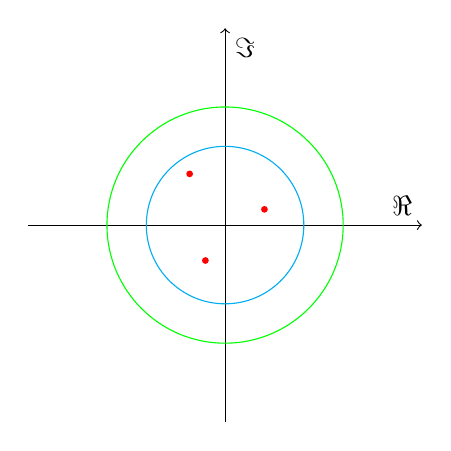
\begin{tikzpicture}[scale=.5]
        % Axis
        \draw [->] (-5,0) -- (5,0) node [above left]  {$\Re$};
        \draw [->] (0,-5) -- (0,5) node [below right] {$\Im$};

        \draw[cyan] (0,0) circle (2);
        \draw[green] (0,0) circle (3);
        
        \filldraw[red] (1,0.4) circle (2pt);
        \filldraw[red] (-0.5, -0.9) circle (2pt);
        \filldraw[red] (-0.9, 1.3) circle (2pt);
    \end{tikzpicture}
\end{center}

Dimostriamo ora il \nameref{th:hirsch}.
\begin{proof}
    Per definizione di autovalore deve esistere un vettore $\vec x \in \C^n$, $\vec x \neq \vec 0$ tale che \[
        A\vec x = \lambda\vec x.
    \] Sia $\norm$ la norma vettoriale che induce la norma matriciale che stiamo considerando: allora \[
        \abs{\lambda} \cdot \norm{\vec x}
        = \norm{\lambda\vec x}
        = \norm{A\vec x}
        \leq \norm{A} \cdot \norm{x}.
    \]

    Siccome $\vec x \neq \vec 0$ si ha che $\norm{\vec x} > 0$, dunque dividendo entrambi i membri per $\norm{\vec x}$ otteniamo \[
        \abs{\lambda} \leq \norm{A}. \qedhere
    \]
\end{proof}

\subsection{Teoremi di Gershgorin}

Vogliamo ora localizzare ancora più precisamente gli autovalori di una matrice.

\begin{definition}{Cerchi di Gershgorin}{}
    Sia $A \in \Mat{\C, n, n}$. Per ogni $1 \leq i \leq n$ definiamo l'$i$-esimo \strong{cerchio di Gershgorin} come l'insieme \[
        K_i \deq \set*{z \in \C \given \abs*{z - a_{ii}} \leq \sum_{j=1, j\neq i}^n \abs{a_{ij}}}.
    \]
\end{definition}

L'$i$-esimo cerchio è quindi dato da tutti i punti la cui distanza da $a_{ii}$ (l'elemento della diagonale nella $i$-esima riga) è minore della somma di tutti gli elementi dell'$i$-esima riga, escluso l'elemento della diagonale. Segue quindi che \begin{itemize}
    \item $a_{ii}$ rappresenta il \emph{centro} del cerchio $K_i$;
    \item $\sum_{j = 1, j\neq i}^n \abs{a_{ij}}$, ovvero la somma degli elementi dell'$i$-esima riga escluso $a_{ii}$, è il \emph{raggio} del cerchio.   
\end{itemize}

\begin{example}
    Consideriamo la matrice \[
        A = \begin{pmatrix}
            -1 & -1 & 0 \\
            -1 & 2  & 1 \\
            2  & 0  & 3 \\
        \end{pmatrix}.
    \] I corrispondenti cerchi di Gershgorin sono \begin{align}
        &K_1 = \set*{z \in \C \given \abs*{z + 1} \leq \abs{-1} + \abs{0} = 1} \\
        &K_2 = \set*{z \in \C \given \abs*{z - 2} \leq \abs{-1} + \abs{1} = 2} \\
        &K_3 = \set*{z \in \C \given \abs*{z - 3} \leq \abs{2} + \abs{0} = 2}.
    \end{align}

    Rappresentiamoli nel piano complesso:
    \begin{center}
        \tikzsetnextfilename{gershgorin_exmpl1}
        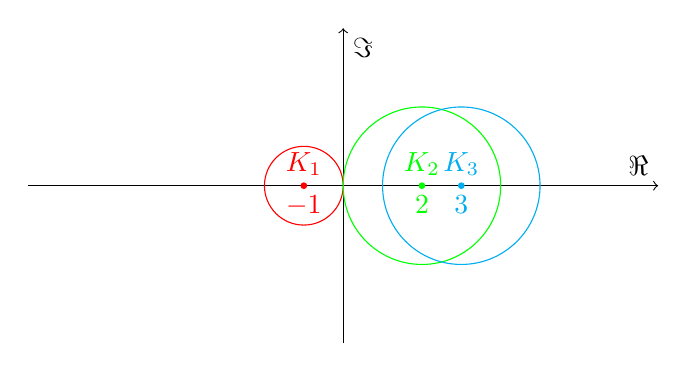
\begin{tikzpicture}[scale=.5]
            % Axis
            \draw [->] (-8,0) -- (8,0) node [above left]  {$\Re$};
            \draw [->] (0,-4) -- (0,4) node [below right] {$\Im$};

            \draw[red] (-1,0)  circle (1) node[above] {$K_1$}; % [$K_1$];
            \draw[green] (2,0) circle (2) node[above] {$K_2$}; % [$K_2$];
            \draw[cyan] (3,0)  circle (2) node[above] {$K_3$}; % [$K_3$];

            \filldraw[red] (-1,0)  node[below] {$-1$} circle (2pt); % [$K_1$];
            \filldraw[green] (2,0) node[below] {$2$}  circle (2pt); % [$K_2$];
            \filldraw[cyan] (3,0)  node[below] {$3$}  circle (2pt); % [$K_3$];
        \end{tikzpicture}
    \end{center}
\end{example}

\begin{theorem}
    {Primo Teorema di Gershgorin}
    {gershgorin_1}
    Sia $A \in \Mat{\C, n, n}$ e $\K_i$ i suoi cerchi di Gershgorin. Allora per ogni $\lambda \in \C$ autovalore di $A$ si ha \[
        \lambda \in \bigunion_{i=1}^n K_i.
    \]
\end{theorem}
\begin{proof}
    Sia $\lambda \in \C$ un autovalore di $A$, ovvero tale che esiste $\vec x \in \C^n$, $\vec x \neq \vec 0$ tale che $A\vec x = \lambda\vec x$. Scrivendo la matrice e i vettori per esteso questo equivale a \[
        \begin{pmatrix}
            a_{11} &\dots  &a_{1n} \\
            \vdots &\ddots &\vdots \\
            a_{n1} &\dots  &a_{nn} \\
        \end{pmatrix} \begin{pmatrix}
            x_1 \\ \vdots \\ x_n
        \end{pmatrix} = \lambda \begin{pmatrix}
            x_1 \\ \vdots \\ x_n
        \end{pmatrix} = \begin{pmatrix}
            \lambda x_1 \\ \vdots \\ \lambda x_n    
        \end{pmatrix}.
    \] Svolgendo il prodotto otteniamo che per ogni riga $1 \leq i \leq n$ vale che \[
        \begin{pmatrix}
            a_{i1} &\dots a_{in}
        \end{pmatrix} \begin{pmatrix}
            x_1 \\ \vdots \\ x_n
        \end{pmatrix} = a_{i1}x_1 + \dots + a_{in}x_n 
        = \sum_{j=1}^n a_{ij}x_j
        = \lambda x_i.
    \] Portando fuori dalla sommatoria il termine corrispondente a $j = i$ otteniamo \begin{align*}
        &\parens*{\sum_{j=1, j\neq i}^n a_{ij}x_j} + a_{ii}x_i = \lambda x_i\\
        \iff {}&\sum_{j=1, j\neq i}^n a_{ij}x_j =  \lambda x_i - a_{ii}x_i
    \end{align*} sempre per ogni $i = 1, \dots, n$.
    
    Sia ora $p$ l'indice per cui \[
        \abs*{x_p} = \norm{\vec x}_\infty = \max_{1 \leq i \leq n} \abs*{x_i},
    \] ovvero $p$ è l'indice della componente di modulo massimo. 
    Siccome $\vec x \neq \vec 0$ sicuramente c'è almeno una componente diversa da $0$, dunque $\abs*{x_p} > 0$. 
    
    Riscrivo quindi l'ultima equazione nel caso particolare di $i = p$: \[
        \sum_{j=1, j\neq p}^n a_{pj}x_j =  \lambda x_p - a_{pp}x_p
    \] che passando ai moduli diventa \[
        \abs*{\lambda - a_{pp}}\cdot \abs*{x_p} 
        = \abs*{\sum_{j=1, j\neq p}^n a_{pj}x_j} 
        \leq \sum_{j=1, j\neq p}^n \abs*{a_{pj}} \cdot \abs*{x_j},
    \] dove all'ultimo passaggio abbiamo usato la disuguaglianza triangolare dei moduli.

    Dividendo per $\abs*{x_p}$ (siccome è sempre strettamente maggiore di $0$) si ha \begin{align*}
        \abs*{\lambda - a_{pp}} 
        &\leq \frac{1}{\abs*{x_p}}\sum_{j=1, j\neq p}^n \abs*{a_{pj}} \cdot \abs*{x_j}\\
        &= \sum_{j=1, j\neq p}^n \abs*{a_{pj}} \cdot \frac{\abs*{x_j}}{\abs*{x_p}}.
        \intertext{Osserviamo ora che $\frac{\abs*{x_j}}{\abs*{x_p}}$ è sempre minore o uguale a $1$: infatti $x_p$ è la componente di modulo massimo, dunque il numeratore della frazione è sempre minore o uguale al denominatore. Si ha quindi}
        \abs*{\lambda - a_{pp}} &\leq \sum_{j=1, j\neq p}^n \abs*{a_{pj}},
    \end{align*} ovvero $\lambda \in K_p$. 

    Siccome $\lambda$ appartiene ad un cerchio di Gershgorin in particolare apparterrà all'unione di tutti i cerchi, come volevasi dimostrare.  
\end{proof}

Possiamo considerare anche i cerchi \emph{per colonne}, ovvero \[
    H_j \deq \set*{z \in \C \given \abs*{z - a_{jj}} \leq \sum_{i = 1, i \neq j}^n \abs*{a_{ij}}}.
\] I cerchi per colonne corrispondono ai cerchi per righe della matrice trasposta $A\trans$: ricordando che ogni matrice ha gli stessi autovalori della sua trasposta si ha che ogni autovalore $\lambda \in \C$ di $A$ deve appartenere all'unione dei cerchi per colonna, ovvero \[
    \lambda \in \bigunion_{j=1}^n H_j.
\] In particolare varrà quindi \[
    \lambda \in \parens*{\bigunion_{i=1}^n K_i} \inters \parens*{\bigunion_{j=1}^n H_j}
\] per ogni $\lambda$ autovalore di $A$.

Enunciamo ora (senza dimostrazione) il \nameref{th:gershgorin_2}.

\begin{theorem}
    {Secondo Teorema di Gershgorin}
    {gershgorin_2}
    Sia $A \in \Mat{\C, n, n}$ tale che $k$ dei cerchi di Gershgorin di $A$ siano disgiunti dai rimanenti $n-k$. Sia inoltre $\KK_1$ l'unione dei $k$ cerchi che formano il primo gruppo e $\KK_2$ l'unione dei rimanenti.

    Allora $k$ autovalori di $A$ appartengono a $\KK_1$, mentre i rimanenti $n-k$ appartengono a $\KK_2$. 
\end{theorem}

\subsection{Predominanza diagonale}

\begin{definition}
    {Matrice a predominanza diagonale}
    Una matrice $A \in \Mat{\C, n, n}$ si dice \strong{a predominanza diagonale per righe} se per ogni riga $i = 1, \dots, n$ si ha \[
        \abs*{a_{ii}} > \sum_{j=1, j\neq i}^n \abs*{a_{ij}},
    \] ovvero se il modulo dell'elemento sulla diagonale $a_{ii}$ è strettamente maggiore della somma dei moduli del resto degli elementi della riga $i$.

    Analogamente $A$ si dice \strong{a predominanza diagonale per colonne} se per ogni colonna $j = 1, \dots, n$ si ha \[
        \abs*{a_{jj}} > \sum_{i=1, i\neq j}^n \abs*{a_{ij}}.
    \] 
\end{definition}

Osserviamo che se $A$ è a predominanza diagonale per righe allora $A\trans$ lo è per colonne, e viceversa.

\begin{proposition}{}{}
    Una matrice a predominanza diagonale (per righe o per colonne) è invertibile.
\end{proposition}
\begin{proof}
    Ricordiamo che una matrice è invertibile se e solo se $0$ non è autovalore: mostriamo quindi che $0$ non appartiene all'unione dei cerchi di Gershgorin.
    Questo implica che un qualsiasi tipo di predominanza diagonale è sufficiente: se mostriamo che una matrice a predominanza diagonale è invertibile (ovvero che $0$ non è autovalore) segue che anche la sua trasposta è invertibile (poiché ha gli stessi autovalori); analogamente se partiamo da una matrice a predominanza diagonale per colonne.

    Sia quindi $A$ una matrice a predominanza diagonale per righe, $1 \leq i \leq n$ qualsiasi e consideriamo l'$i$-esima riga della matrice $A$. Si ha \[
        \abs*{0 - a_{ii}} = \abs*{a_{ii}} > \sum_{j=1, j\neq i}^n \abs*{a_{ij}},
    \] dunque $0$ non appartiene all'$i$-esimo cerchio di Gershgorin.

    Siccome $0 \notin K_i$ per ogni $i$ segue anche che $0 \notin \bigunion K_i$, ovvero $0$ non può essere autovalore (per il \nameref{th:gershgorin_1}).
\end{proof}
\chapter{Risoluzione di sistemi lineari}
\section{Fattorizzazione LU}

Abbiamo già iniziato a parlare di sistemi lineari e della loro risoluzione precedentemente. Dopo averne studiato il condizionamento studiamo degli algoritmi per trovare efficientemente le soluzioni di sistemi della forma $A\vec x = \vec b$, dove $A$ è una matrice, $\vec b$ è il vettore dei termini noti e $\vec x$ è il vettore delle incognite.

\subsection{Risoluzione di un sistema triangolare}

Se la matrice $A$ è triangolare superiore è particolarmente semplice risolvere il sistema, in quanto possiamo usare la tecnica di \strong{sostituzione all'indietro}.

\[
    \begin{pmatrix}
        a_{11}  &\dots  &a_{1n} \\
                &\ddots &\vdots \\
                &       &a_{nn}
    \end{pmatrix} \begin{pmatrix}
        x_1 \\ \vdots \\ x_n
    \end{pmatrix} = \begin{pmatrix}
        b_1 \\ \vdots \\ b_n
    \end{pmatrix}
\]

Infatti l'ultima riga ci fornisce l'equazione $a_{nn}x_n = b_n$, da cui ricaviamo $x_n = \dfrac{b_n}{a_{nn}}$ (a patto che $a_{nn}$ sia diverso da $0$); usando questo risultato possiamo risolvere l'equazione della penultima riga, cioè \[
    a_{n-1, n-1}x_{n-1}+a_{n-1,n}x_n = b_{n-1},
\] che diventa \[
    x_{n-1} = \frac{b_{n-1} - a_{n-1,n}x_n}{a_{n-1,n-1}}.
\]

In generale, tramite questo metodo, la formula per calcolare $x_k$ è \[
    x_k = \frac{\displaystyle b_k - \sum_{j=k+1}^n a_{kj}x_j}{a_{kk}}.
\]

Un programma MatLab che esprime questo algoritmo è il seguente:
\begin{minted}{MatLab}
    % given an upper triangular matrix A of order n
    % and a n-dimensional vector b
    % it calculates the solution of the system |$A\vec x = \vec b$|
    function x = upp_triang_solve(A, b)
        x(n) = b(n) / A(n, n)
        for k = n-1 : -1 : 1
            s = 0
            for j = k+1 : n
                s = s + A(k, j)*x(j)
            end
            x(k) = (b(k) - s) / A(k, k)
        end
    end
\end{minted}

Una veloce analisi del costo computazionale dell'algoritmo ci dice che esso ha costo, al caso pessimo, di $\OO(n^2)$: infatti il ciclo interno ha costo $\OO(n - k)$, e viene ripetuto per $k = 1, \dots, n-1$, da cui viene il costo \[
    \sum_{k=1}^{n-1} \OO(n-k) = \OO(n^2).
\] Questo costo non è migliorabile: infatti la matrice ha $\OO(n^2)$ elementi, da cui non è possibile diminuire il numero di operazioni fatte.

Se la matrice è triangolare inferiore possiamo usare la stessa tecnica ma partendo dalla prima riga, tramite la \strong{sostituzione all'avanti}.

\subsection{Mosse di Gauss e fattorizzazione LU}

Se la matrice $A$ non è triangolare il metodo più usato per risolvere il sistema $A\vec x = \vec b$ è l'\strong{algoritmo di Gauss}, che sfrutta le cosiddette mosse di Gauss.

\begin{definition}
    {Mosse di Gauss}{mosse_gauss}
    Sia $A \in \Mat{\F, n, n}$ una matrice. Una \strong{mossa di Gauss per riga} è un'operazione sulle righe della matrice con una delle seguenti forme:
    \begin{enumerate}[(1)]
        \item scambiare la riga $i$ con la riga $j$;
        \item moltiplicare la riga $i$ per un coefficiente $\alpha \in \F$, $\alpha \neq 0$;
        \item sottrarre alla riga $i$ la riga $j$ moltiplicata per un coefficiente $\alpha$.   
    \end{enumerate} 
\end{definition}

La strategia è quindi quella di applicare ripetutamente le mosse di Gauss (secondo il cosiddetto \strong{algoritmo di Gauss}) per ridurre la matrice $A$ ad una matrice $U$ triangolare superiore: \[
    [A | \vec b] = [A^{(0)} | \vec b^{(0)}] \leadsto [A^{(1)} | \vec b^{(1)}] \leadsto \dots \leadsto [A^{(n-1)} | \vec b^{(n-1)}] = [U | \vec y].
\]

Mostreremo nella prossima sezione che in alcuni casi particolari possiamo descrivere una singola mossa di Gauss come un prodotto tra matrici \[
    A^{(k+1)} = E^{(k+1)}A^{(k)}
\] dove $E^{(k+1)}$ sarà una matrice invertibile e triangolare inferiore.

In tal caso segue quindi che \[
    U = A^{(n-1)} = E^{(n-1)}A^{(n-2)} = E^{(n-1)}E^{(n-2)}A^{(n-3)} = \dots = E^{(n-1)}\cdots E^{(1)}A.
\] Siccome abbiamo detto che tutte le matrici $E^{(i)}$ sono invertibili anche il loro prodotto lo sarà: chiamiamo dunque \[
    L\inv \deq E^{(n-1)}\cdots E^{(1)},
\] da cui segue che $U = L\inv A$, ovvero $A = LU$.

Il sistema $A\vec x = \vec b$ diventa quindi $LU\vec x = \vec b$, che può essere risolto come \[
    \left\{ 
        \;
        \begin{aligned}
            &L\vec y = \vec b \\
            &U\vec x = \vec y
        \end{aligned}
    \right.
\] 
Sappiamo che $U$ è triangolare superiore, dunque possiamo risolvere il sistema $U\vec x = \vec y$ usando i metodi studiati precedentemente.
Allo stesso modo, dato che $L$ è data dal prodotto di matrici triangolari inferiori anch'essa è triangolare inferiore, dunque possiamo risolvere anche il sistema $L\vec y = \vec b$ efficientemente, trovando quindi una soluzione al sistema originale.
% Tuttavia per ricavare $\vec y$ dobbiamo risolvere il primo sistema: mostrando che anche $L$ è triangolare riusciremmo a trovare molto velocemente una soluzione alla prima equazione, e quindi all'intero sistema.

Siamo quindi interessati a studiare in che modo e in quali casi si può scrivere $A$ come prodotto di due matrici, di cui una è triangolare inferiore ($L$, da \emph{lower triangular}) e una è triangolare superiore ($U$, da \emph{upper triangular}). Diamo dunque la seguente definizione.

\begin{definition}
    {Fattorizzazione LU}{LU-fact}
    Sia $A \in \Mat{\F, n, n}$ una matrice. Si dice che $A$ è \strong{fattorizzabile LU} se esistono due matrici $L, U \in \Mat{\F, n, n}$ tali che \begin{enumerate}[(1)]
        \item $L$ è triangolare inferiore ed ha tutti $1$ sulla diagonale principale;
        \item $U$ è triangolare superiore;
        \item vale che \[
            A = LU.
        \]
    \end{enumerate} 
\end{definition}

% Il nostro scopo sarà quindi quello di trovare condizioni per cui una matrice $A$ può essere fattorizzata in modo LU, fattorizzarla e risolvere il sistema separando la parte triangolare superiore e quella triangolare inferiore.

Il seguente Teorema ci dà delle condizioni sufficienti sulla fattorizzabilità.

\begin{theorem}
    {Esistenza e unicità della fattorizzazione LU}{exist-unique-LU-fact}
    Sia $A \in \Mat{\F, n, n}$. Se le sottomatrici principali di testa di $A$ di ordine $k$, con $k = 1, \dots, n-1$, sono invertibili, allora $A$ è fattorizzabile LU e tale fattorizzazione è unica.  
\end{theorem}
\begin{proof}
    Dimostriamo la tesi per induzione su $n$.
    \newthought{Caso base} Supponiamo $n = 1$. Allora la matrice $A = \begin{bmatrix}
        a_{11}
    \end{bmatrix}$ non ha sottomatrici, dunque la condizione è vacuamente verificata. Inoltre \begin{itemize}
        \item una possibile fattorizzazione di $A$ è data da \[
            L = \begin{bmatrix} 1 \end{bmatrix}, \qquad
            U = \begin{bmatrix} a_{11} \end{bmatrix}
        \]
        \item tale fattorizzazione è unica: infatti $L$ deve essere la matrice con un singolo $1$ poiché sulla diagonale non può avere valori diversi, da cui segue che $U = A$.
    \end{itemize}
    La tesi è quindi verificata nel caso base.

    \newthought{Passo induttivo} Supponiamo che la tesi sia vera per matrici di ordine $m$, per ogni $m < n$, e mostriamola per $n$.

    Supponiamo quindi che $A$ abbia sottomatrici di testa non singolari. Per mostrare che $A$ sia fattorizzabile LU dobbiamo trovare due matrici $L, U$ che rispettano le condizioni sulla fattorizzazione. Scrivendole a blocchi, si ha \[
        % A = \left( \begin{array}{@{}c|c@{}}
        %     A_{n-1} & \vec z \\\hline
        %     \vec x\trans & a_{nn}
        % \end{array}\right)
        % A = \begin{array}{@{}c@{}c@{}c|c@{}}
        %     \hphantom{a_{ii}} &             &\hphantom{a_{ii}}   & \\
        %     \hphantom{a_{ii}} &A_{n-1}      &\hphantom{a_{ii}}   &\vec z \\
        %     \hphantom{a_{ii}} &             &\hphantom{a_{ii}}   & \\ 
        %         \hline \rule{0pt}{1.1\normalbaselineskip}
        %     \hphantom{a_{ii}} &\vec x\trans &\hphantom{a_{ii}}   &a_{nn}
        % \end{array}
        A = 
        % \begin{pNiceArray}{ccc|c}
        %     \Block{3-3}<\Large>{A_{n-1}} &             &   & \\
        %      &      &   &\vec z \\
        %      &             &   & \\ 
        %         \hline \rule{0pt}{1.1\normalbaselineskip}
        %      &\vec x\trans &   &a_{nn}
        % \end{pNiceArray}
        \left( \begin{array}{@{}ccc|c}
            \; &             &\;   & \\
            \; &A_{n-1}      &\;   &\vec z \\
            \; &             &\;   & \\ 
                \hline \rule{0pt}{1.1\normalbaselineskip}
            \; &\vec x\trans &\;   &a_{nn}\;
        \end{array}\right)
        =
        \left( \begin{array}{@{}ccc|c}
            \; &             &\;   & \\
            \; &\widehat{L}  &\;   &\vec 0 \\
            \; &             &\;   & \\ 
                \hline \rule{0pt}{1.1\normalbaselineskip}
            \; &\vec w\trans &\;   &1\;
        \end{array}\right)
        \left( \begin{array}{@{}ccc|c}
            \; &             &\;   & \\
            \; &\widehat{U}  &\;   &\vec y \\
            \; &             &\;   & \\ 
                \hline \rule{0pt}{1.1\normalbaselineskip}
            \; &\vec 0\trans &\;   &\beta\;
        \end{array}\right)
    \] dove $A_{n-1}, \vec z, \vec x\trans, a_{nn}$ sono noti, mentre $\widehat{L}, \widehat{U}, \vec w\trans, \vec y$ e $\beta$ sono incognite.  

    Svolgendo il prodotto a blocchi devono quindi valere le seguenti condizioni: \[
        \left\{
            \!\!\!\!\!\!\!
            \begin{aligned}
                &&A_{n-1} &= \widehat{L}\widehat{U} + \vec 0\vec 0\trans = \widehat{L}\widehat{U} \\
                &&\vec z &= \widehat{L}\vec y + \beta\vec 0 = \widehat{L}\vec y\\
                &&\vec x\trans &= \vec w\trans \widehat{U} + 1\cdot \vec 0\trans = \vec w\trans \widehat{U}\\
                &&a_{nn} &= \vec w\trans \vec y + \beta.
            \end{aligned}
        \right.
    \]

    \begin{enumerate}[(1)]
        \item Osserviamo che la prima equazione corrisponde alla fattorizzazione LU di $A_{n-1}$. 
        Siccome $A_{n-1}$ è la sottomatrice di testa di $A$ di ordine $n-1$ le sue sottomatrici di testa sono uguali alle sottomatrici di testa di $A$, dunque sono invertibili per ipotesi.   

        Per l'ipotesi induttiva segue quindi che la fattorizzazione LU di $A_{n-1}$ esiste ed è unica, dunque $\widehat{L}, \widehat{U}$ esistono e sono uniche.
        \item Siccome la matrice $\widehat{L}$ è triangolare inferiore segue che il suo determinante è il prodotto degli elementi della diagonale, ovvero $\det \widehat{L} = 1$. Segue quindi che il sistema $\widehat{L}\vec y = \vec z$ ammette una e una sola soluzione, dunque $\vec y$ è univocamente determinato.  
        \item Applicando l'operatore di trasposizione ad entrambi i membri dell'equazione si ottiene il sistema equivalente \[
            \widehat{U}\trans \vec w = \vec x.
        \] La matrice $\widehat{U}\trans$ è invertibile: infatti $A_{n-1} = \widehat{L}\widehat{U}$ e $\widehat{L}$ invertibile implica che $\widehat{U} = \widehat{L}\inv A_{n-1}$. Per il Teorema di Binet segue quindi che \[
            \det \widehat{U} = \det \widehat{L}\inv \cdot \det A_{n-1}.
        \] $\widehat{L}\inv$ è certamente invertibile, mentre $A_{n-1}$ è invertibile in quanto è la sottomatrice di testa di $A$ di ordine $n-1$, e per ipotesi tutte le sottomatrici di testa di $A$ sono invertibili.

        Segue quindi che $\widehat{U}$ è invertibile, da cui anche $\widehat{U}\trans$ è invertibile, dunque il vettore $\vec w$ esiste ed è unico.
        \item L'ultima equazione è equivalente a \[
            \beta = a_{nn} - \vec w\trans\vec y.
        \] Abbiamo dimostrato che $\vec w$ e $\vec y$ esistono e sono unici, dunque anche $\beta$ esiste ed è univocamente determinato.
    \end{enumerate}

    Segue quindi che la matrice $A$ è fattorizzabile LU, da cui la tesi.
\end{proof}
\section{Algoritmo di Gauss}

Durante lo studio della fattorizzazione LU abbiamo fatto l'ipotesi che, in alcune condizioni, ogni mossa di Gauss può essere rappresentata dalla moltiplicazione a sinistra per una qualche matrice invertibile e triangolare inferiore.

Vogliamo ora dare una formalizzazione dell'algoritmo di Gauss che ci spiega quali sono queste matrici, come sono fatte, perché funzionano e in quali condizioni esistono.

Ricordiamo che l'algoritmo di Gauss per ridurre a scalini (cioè ad una matrice triangolare superiore) funziona così:
\begin{enumerate}[1.]
    \item sia $A \in \Mat{\R, n, n}$ una matrice invertibile, poniamo $k \deq 1$; 
    \item consideriamo l'elemento in posizione $(k, k)$: se è nullo scambiamo la riga $k$ con una riga successiva;
    \item per ogni riga $i$ successiva alla $k$-esima, sottraiamo da $R_i$ la riga $R_k$ moltiplicata per $\frac{a_{ik}}{a_{kk}}$: in questo modo annulliamo tutti gli elementi della colonna $k$-esima che sono dopo la riga $k$;
    \item poniamo $k \deq k+1$ e torniamo al passo \texttt{2.} 
\end{enumerate}

Definiamo ora il tipo di matrici che sfrutteremo per trasformare questo calcolo sulle righe in un'operazione di prodotto matriciale.

\begin{definition}
    {Matrice elementare di Gauss}{matr_elem_Gauss}
    Sia $E \in \Mat{\R, n, n}$. $E$ si dice \strong{matrice elementare di Gauss} se esistono $k \in \N$, $\vec v \in \R^n$ tali che 
    \begin{enumerate}
        \item $\vec v$ è nullo nelle prime $k$ posizioni, ovvero \[
            v_1 = \dots = v_k = 0,
        \]
        \item si ha \[
            E = I_n - \vec v\vec{e}\trans_k,
        \] dove $\vec{e}_k$ è il $k$-esimo vettore della base canonica di $\R^n$. 
    \end{enumerate}  
\end{definition}

\begin{example}
    Se $k = 2$ ad esempio otteniamo \begin{align*}
        E &= I_n - \vec v\vec{e}\trans_2 \\[1em]
        &= I_n - \begin{psmallmatrix}
            0 \\ 0 \\ v_3 \\ \vdots \\ v_k
        \end{psmallmatrix}\begin{psmallmatrix}
            0 & 1 & 0 & \dots & 0
        \end{psmallmatrix} \\
        &= 
        % \begin{psmallmatrix}
        %     1 &  &  &       &\\
        %       &1 &  &       &\\
        %       &  &1 &       &\\
        %       &  &  &\ddots &\\
        %       &  &  &       &1
        % \end{psmallmatrix} 
        \begin{bmatrix}
            1 & &\\
              &\ddots &\\
              & &1
        \end{bmatrix}
        - \begin{bmatrix}
            0 &         &       &       &\\
              & 0       &       &       &\\
              & -v_3    &0      &       &\\
              & \vdots  &       &\ddots &\\
              & -v_n    &       &       &0
        \end{bmatrix} \\
        &= \begin{bmatrix}
            1 &         &       &       &\\
              & 1       &       &       &\\
              & -v_3    &1      &       &\\
              & \vdots  &       &\ddots &\\
              & -v_n    &       &       &1
        \end{bmatrix}.
    \end{align*}
\end{example}

\subsubsection{Proprietà delle matrici elementari di Gauss} 
Le matrici elementari di Gauss hanno diverse proprietà che ci torneranno utili nel dimostrare che effettivamente modellano l'algoritmo di Gauss.

\begin{proposition}
    {Proprietà delle Matrici Elementari di Gauss}{matr_elem_Gauss_prop}
    \begin{enumerate}[(1)]
        \item Le matrici elementari di Gauss sono triangolari inferiori, e gli elementi della diagonale sono tutti uguali ad $1$.
        \item Le matrici elementari di Gauss sono invertibili. Inoltre, se $E = I_n - \vec v\vec{e}\trans_k$ è una matrice elementare di Gauss, allora la sua inversa è ancora una matrice elementare di Gauss, data da \[
            E\inv = I_n + \vec v\vec e\trans_k.
        \]
        \item Dato $x \in \R^n$ con $x_k \neq 0$ esiste una matrice elementare di Gauss $E$ tale che \[
            E\vec x = (x_1, \dots, x_k, 0, \dots, 0)\trans.
        \] La matrice è della forma $E = I_n - \vec v\vec e\trans_k$, dove \[
            \vec v = \parens*{0, \dots, 0, \frac{x_{k+1}}{x_k}, \dots, \frac{x_n}{x_k}}\trans.
        \]
        \item Siano $E_k = I_n - \vec v\vec e\trans_k$, $E_h = I_n - \vec w\vec e_h\trans$ due matrici elementari di Gauss, con $h > k$. Allora \[
            E_kE_h = I_n - \vec v\vec e_k\trans - \vec w\vec e_h\trans.
        \]
        \item Sia $\vec y \in \R^n$, $E_k$ una matrice elementare di Gauss. Allora il calcolo di $E_k\vec y$ ha un costo computazionale di $\OO(n - k)$ flops (\emph{floating point operations}). 
    \end{enumerate}
\end{proposition}

Dimostriamo separatamente le varie proprietà.

\begin{proof}[Dimostrazione della Proprietà (1)]
    È sufficiente dimostrare che $\vec v\vec e_k\trans$ sia triangolare inferiore con gli zeri sulla diagonale, poiché da questo segue che $E = I_n - \vec v\vec e_k\trans$ è triangolare inferiore con $1$ sulla diagonale. 
    
    Siano quindi $i, j \in \N$ con $i \leq j \leq n$ due indici e mostriamo che $e_{ij}$, ovvero l'elemento della matrice $E$ in posizione $(i, j)$ (che osserviamo essere un elemento sulla diagonale o sopra la diagonale, in quanto abbiamo richiesto che $j \geq i$) è uguale a $0$.

    Per definizione di prodotto tra matrici si ha che \[
        e_{ij} = v_i \cdot \delta_{jk}
    \] dove \[
        \delta_{jk} \deq \begin{cases}
            1, &\text{se } j = k \\
            0, &\text{se } j \neq k 
        \end{cases}
    \] è l'elemento di posizione $j$-esima del vettore $\vec e_k$.

    Consideriamo due casi: \begin{itemize}
        \item se $i \leq k$ allora $v_i = 0$ per definizione di matrice elementare di Gauss, dunque $e_{ij} = 0$;
        \item se $i > k$ allora $j \geq i > k$, dunque $\delta_{jk} = 0$ (poiché $j$ è strettamente maggiore di $k$), dunque $e_{ij} = 0$.   
    \end{itemize}

    Segue quindi la tesi.
\end{proof}
\begin{proof}[Dimostrazione della Proprietà (2)]
    Dalla proprietà (1) segue che il determinante di una matrice elementare è il prodotto degli elementi sulla diagonale poiché è triangolare inferiore, cioè è $1$ e dunque le matrici elementari di Gauss sono invertibili.
    
    Mostriamo ora che l'inversa di $E = I_n - \vec v\vec e_k\trans$ è effettivamente $E\inv = I_n + \vec v\vec e_k\trans$.
    \begin{align*}
        EE\inv &= (I_n - \vec v\vec e_k\trans)(I_n + \vec v\vec e_k\trans) \\
        &= I_n + \vec v\vec e_k\trans - \vec v\vec e_k\trans - \vec v\vec e_k\trans\vec v\vec e_k\trans \\
        &= I_n - \vec v\vec e_k\trans\vec v\vec e_k\trans.
    \end{align*}

    Per mostrare che $EE\inv$ è l'identità basta quindi mostrare che $\vec v\vec e_k\trans\vec v\vec e_k\trans$ è la matrice nulla. Osserviamo innanzitutto che per associatività del prodotto tra matrici \[
        \vec v\vec e_k\trans\vec v\vec e_k\trans = \vec v(\vec e_k\trans\vec v)\vec e_k\trans
    \] e il termine tra parentesi è uno scalare, per cui commuta con il prodotto tra matrici, ottenendo \[
        (\vec e_k\trans\vec v) \cdot \vec v\vec e_k\trans.
    \]

    Per definizione di prodotto tra vettori si ha che \[
        \vec e_k\trans\vec v = \sum_{i=1}^n \delta_{ik}v_i.
    \] Distinguiamo ora due casi:
    \begin{itemize}
        \item quando $i \neq k$ si ha che $\delta_{ik} = 0$, dunque $\delta_{ik}v_i = 0$;
        \item quando $i = k$ si ha che $v_i = 0$ (poiché $\vec v$ è nullo nelle prime $k$ posizioni), dunque $\delta_{ik}v_i = 0$.    
    \end{itemize}

    Segue quindi che tutti i termini della somma sono nulli, da cui $\vec e_k\trans\vec v = 0$, dunque $EE\inv = I_n$ come volevamo.
\end{proof}

\begin{proof}
    [Dimostrazione della Proprietà (3)]
    \label{proof:prop_3_Gauss}
    Poniamo $\vec v = (0, \dots, 0, v_{k+1}, \dots, v_n)$ e dimostriamo che per ogni $i > k$ si ha che \[
        v_i = \frac{x_i}{x_k}.
    \] Per definizione di matrice elementare di Gauss si ha che \[
        E\vec x = \begin{bNiceMatrix}[columns-width = 0.4cm]
            1 &         &         &  & &\\
              &\Ddots   &         &  & &\\
              &         &1         &  & &\\
              &         &-v_{k+1} & & &\\
              &         &\Vdots   &  & &\\
              &         &-v_n     &  &       &1
            % \CodeAfter \line[shorten=6pt]{3-3}{4-4}
            \CodeAfter \line{3-3}{6-6}
        \end{bNiceMatrix} \begin{pmatrix}
            x_1 \\ \smallvdots \\ x_{k} \\ x_{k+1} \\ \smallvdots \\ x_n 
        \end{pmatrix} \stackrel{!}{=} \begin{pmatrix}
            x_1 \\ \smallvdots \\ x_{k} \\ 0 \\ \smallvdots \\ 0 
        \end{pmatrix}.
    \]
    Considerando questo prodotto tra matrici come un sistema lineare (le cui incognite però sono i $v_i$), le prime $k$ righe corrispondono alle equazioni \[
        1 \cdot x_i = x_i,
    \] che sono banalmente verificate.

    Sia quindi $i > k$. L'equazione codificata dalla riga $i$-esima è dunque \[
        -v_ix_k + 1\cdot x_i = 0,
    \] da cui ricaviamo che \[
        v_i = \frac{x_i}{x_k},
    \] come volevamo.
\end{proof}

% \begin{proof}
%     [Dimostrazione della Proprietà (4)]
% \end{proof}

\begin{proof}
    [Dimostrazione della Proprietà (5)]
    Sia $\vec z \deq E_k \vec y$. Allora \[
        \vec z = (I_n - \vec v \vec e_k\trans)\cdot \vec y = \vec y - \vec v \vec e_k\trans \vec y = \vec y - y_k \vec v,
    \] dove $y_k$ è la $k$-esima coordinata del vettore $\vec y$, e l'ultima uguaglianza viene dal fatto che il prodotto del trasposto del $k$-esimo vettore della base canonica (cioè $\vec e_k\trans$) con un qualsiasi altro vettore $\vec w \in \R^n$ dà come risultato la $k$-esima coordinata di $\vec w$.
    
    Ma allora \[
        z_i = \begin{cases}
            y_i, &\text{se } i \leq k \\
            y_i - y_kv_i, &\text{se } i > k.
        \end{cases} 
    \] Per calcolare la coordinata $i$-esima (con $i > k$) di $\vec z$ abbiamo quindi bisogno di $2$ operazioni floating point (un prodotto e una differenza) e le coordinate di indice maggiore di $k$ sono $n-k$, dunque in totale abbiamo bisogno di un numero di operazioni nell'ordine di $\OO(n - k)$. 
\end{proof}

\subsection{Algoritmo di Gauss tramite matrici elementari}

Possiamo ora dimostrare che l'algoritmo di Gauss può essere espresso come una sequenza di moltiplicazioni a sinistra per delle matrici elementari di Gauss.

Sia innanzitutto $A \in \Mat{\R, n, n}$ una matrice e definiamo $A^{(k)}$ come la matrice ottenuta al $k$-esimo passo dell'algoritmo di Gauss (in particolare quindi $A = A^{(0)}$).

Dato che ad ogni passo azzeriamo tutti gli elementi della matrice sotto la diagonale, la matrice $A^{(k-1)}$ sarà della forma \[
    A^{(k-1)} = \begin{bNiceMatrix}
        a_{11}^{(k-1)} & &  &\Block{4-3}<\HUGE>{\ast}&&&\\
        &\Ddots & &&&&\\
        & &a_{k-1, k-1}^{(k-1)} & &&&\\
        & & &a_{kk}^{(k-1)} & &&\\
        \Block{3-3}<\HUGE>{0}& & &a_{k+1,k}^{(k-1)} &\Ddots & &\\
        & & &\Vdots &\Block{2-2}<\Huge>{\ast} & & \\
        & & &a_{nk}^{(k-1)} & &\hphantom{a_{nn}^{(k-1)}} &a_{nn}^{(k-1)}
    \end{bNiceMatrix}
\] dove l'area contrassegnata da $0$ contiene tutti zeri, mentre le aree contrassegnate da $\ast$ contengono gli altri elementi della matrice, che possono essere uguali o diversi da $0$. 

Il nostro scopo è ottenere la matrice $A^{(k)}$, in cui sono azzerati anche tutti gli elementi della colonna $k$-esima che si trovano al di sotto dell'elemento della diagonale (ovvero di $a_{kk}$).

Per far ciò sfruttiamo la Proprietà (3): supponendo che $a_{kk}^{(k-1)} \neq 0$ possiamo considerare la matrice elementare di Gauss \[
    E_k \deq I_n - \vec m^{(k)}\vec e_k\trans,
\] dove \[
    m_i^{(k)} = \begin{cases}
        0, &\text{se } i \leq k\\[1em]
        \displaystyle \frac{a_{ik}^{(k-1)}}{a_{kk}^{(k-1)}}, &\text{se } i > k.
    \end{cases}
\] Tale matrice elementare (per la proprietà (3)) annulla tutti i valori sotto $a_{kk}^{(k-1)}$. 

Consideriamo allora il prodotto $E_kA^{(k-1)}$: se $\vec A_1^{(k-1)}, \dots, \vec A_n^{(k-1)}$ sono le colonne di $A^{(k-1)}$ si ha che  
\begin{align*}
    E_kA^{(k-1)} &= E_k \cdot \begin{bNiceMatrix}[vlines]
        \vec A_1^{(k-1)} & \dots & \vec A_k^{(k-1)} & \dots & \vec A_n^{(k-1)}   
    \end{bNiceMatrix} \\
    &= \begin{bNiceMatrix}[vlines]
        E_k\vec A_1^{(k-1)} & \dots & E_k\vec A_k^{(k-1)} & \dots & E_k\vec A_n^{(k-1)}
    \end{bNiceMatrix}.
\end{align*}

A questo punto possiamo notare che \begin{itemize}
    \item se $i < k$ il prodotto $E_k\vec A_i^{(k-1)}$ è uguale a $A_i^{(k-1)}$, ovvero moltiplicare per $E_k$ \strong{non cambia le prime $k-1$ colonne di $A$}: 
    infatti il calcolo fatto nella Dimostrazione della Proprietà (3) notiamo che i primi $k$ elementi vengono sempre mantenuti, mentre i successivi (gli elementi di posto $j = k+1, \dots, n$) vengono aggiornati tramite la legge \[
        a_{ij}^{(k-1)} - m_{j}^{(k)}a_{ik}^{(k-1)}.
    \] Tuttavia, siccome $a_{ik}^{(k-1)} = 0$ segue che anche gli elementi di posto successivo al $k$-esimo rimangono invariati;
    \item se $i = k$ il prodotto $E_k\vec A_i^{(k-1)}$ \strong{azzera tutti gli elementi sotto} $a_{kk}^{(k-1)}$ (l'abbiamo definita proprio per questo scopo);
    \item se $i > k$ il prodotto $E_k\vec A_i^{(k-1)}$ cambia solo gli elementi \strong{al di sotto della $k$-esima riga} (per lo stesso motivo delle prime $k$ colonne). 
\end{itemize}
Dunque la matrice $A^{(k)}$, che corrisponde al $k$-esimo passaggio dell'algoritmo di Gauss, è data da \[
    A^{(k)} \deq E_kA^{(k-1)}.
\] 

Studiamo quindi come sono fatti gli elementi di $A^{(k)}$: essi sono \[
    a_{ij}^{(k)} = \begin{cases}
        a_{ij}^{(k-1)}, &\text{se } i = 1, \dots, k,\qquad j = 1, \dots, n \\[0.8em]
        a_{ij}^{(k-1)} = 0, &\text{se } i = k+1, \dots, n,\; j = 1, \dots, k-1 \\[0.8em]
        0, &\text{se } i = k+1, \dots, n,\; j = k \\[0.8em]
        a_{ij}^{(k-1)} - m_i^{(k)}a_{kj}^{(k-1)}, &\text{se } i = k+1, \dots, n,\; j = k+1, \dots, n \\
    \end{cases}
\]

Questo è effettivamente quello che si fa quando si calcola l'algoritmo di Gauss applicando le mosse per righe. Segue quindi che il metodo per risolvere un sistema lineare $A\vec x = \vec b$ consiste nel moltiplicare ripetutamente a sinistra per le matrici elementari definite sopra: \[
    A\vec x = \vec b \leadsto E_1A\vec x = E_1\vec b \leadsto \dots \leadsto (E_{n-1}\cdots E_1A)\vec x = E_{n-1}\cdots E_1\vec b.
\] 

Notiamo che così facendo dobbiamo anche trasformare il vettore dei termini noti $\vec b$, che al passo $k$-esimo diventerà \[
    b_i^{(k)} \deq \begin{cases}
        b_i^{(k-1)}, &\text{se } i \leq k\\
        b_i^{(k-1)} - m_i^{(k)}b_k^{(k-1)}, &\text{se } i > k.
    \end{cases}
\]

La matrice $U \deq E_{n-1}\cdots E_1A = A^{(n-1)}$ ricavata all'ultimo passo è triangolare superiore, quindi possiamo risolvere il sistema \[
    U\vec x = \vec b^{(n-1)}.
\] Ancora meglio, possiamo sfruttare quanto fatto finora per fattorizzare la matrice $A$ in forma LU.

Infatti, come abbiamo visto nella sezione precedente, possiamo considerare la matrice \[
    L\inv \deq E_{n-1}\cdots E_2E_1,
\] ovvero \[
    L = E_1\inv E_2\inv \cdots E_{n-1}\inv.
\] Per la proprietà (2), ognuna delle matrici $E_i\inv$ è una matrice elementare di Gauss; inoltre per la proprietà (4) le matrici sono moltiplicate nell'\emph{ordine corretto}, dunque possiamo calcolare $L$ senza svolgere i prodotti.
Vale quindi la seguente

\begin{proposition}
    {}{}
    Se l'algoritmo di Gauss è applicabile (ovvero se $a_{ii}^{(i-1)} \neq 0$ per ogni $i = 1, \dots, n-1$) allora $A$ è fattorizzabile LU e \[
        L = \begin{pNiceMatrix}
            1          &          &  &\\
            m_1^{(1)}  &\Ddots    &  &\\
            \Vdots     &m_2^{(2)} &  &\\
                       &\Vdots    &\Ddots & &\\
            m_n^{(1)}  &m_n^{(2)} &\Ldots &m_n^{(n-1)} &1
        \end{pNiceMatrix}.
    \]
\end{proposition}

In particolare la condizione su $A$ vista in questa sezione, ovvero che $a_{ii}^{(i-1)}$ sia non zero per ogni $i = 1, \dots, n-1$, e la condizione sufficiente per la fattorizzazione LU sono equivalenti, come confermato dal seguente Teorema (che non dimostreremo).

\begin{proposition}
    {}{}
    Sia $A \in \Mat{\R, n, n}$ e sia $A_{(k)}$ la matrice ottenuta al $k$-esimo passo dell'algoritmo di Gauss. Vale che le sottomatrici principali di testa di $A$ di ordine $k$ (per $k = 1, \dots, n-1$) sono tutte invertibili se e solo se $a_{kk}^{(k-1)} \neq 0$ per ogni $k = 1, \dots, n-1$.  
\end{proposition}

\subsection{Costo computazionale dell'Algoritmo di Gauss}

Calcoliamo il costo computazionale dell'algoritmo di Gauss. 

Al passo $k$-esimo (in cui passiamo da $A^{(k-1)}$ a $A^{(k)} \deq E_kA^{(k-1)}$) dobbiamo calcolare:
\begin{itemize}
    \item il vettore dei moltiplicatori $m^{(k)}$,
    %  di questo vettore dobbiamo calcolare le ultime $n-k$ componenti (il resto sono tutti $0$) e ogni componente si calcola tramite una singola divisione, quindi dobbiamo fare $n-k$ divisioni;
    \item gli elementi di indice $(i, j)$ con $i = k+1, \dots, n$, $j = k+1, \dots, n$.
\end{itemize}

Per quanto riguarda il vettore dei moltiplicatori, esso ha $n-k$ componenti non nulle e ognuna di queste componenti è calcolabile con una singola divisione, dunque sono sufficienti $n-k$ operazioni.

Invece per gli elementi che vengono modificati al passaggio $k$-esimo ricordiamo che \[
    a_{ij}^{(k)} = a_{ij}^{(k-1)} - m_i^{k-1}a_{kj}^{k-1}.
\] Dunque per ognuno di essi abbiamo bisogno di $2$ operazioni (un prodotto e una differenza), e vi sono $(n-k)^2$ elementi con indici nell'intervallo richiesto, dunque sono necessarie $2(n-k)^2$ operazioni.

Per svolgere tutti i passi dell'algoritmo di Gauss avremo quindi bisogno di \[
    \sum_{k=1}^{n-1} (n-k) + 2(n-k)^2
\] operazioni floating point.
Ponendo $i \deq n-k$ otteniamo quindi \begin{align*}
    &\sum_{i=1}^{n-1} i + 2\sum_{i=1}^{n-1} i^2 \\
    = {}&\frac{n(n-1)}{2} + 2\frac{n(n-1)(2n-1)}{6} \\
    = {}&\frac{n^3}{3} + \OO(n^2),
\end{align*} che è il costo computazionale dell'algoritmo di Gauss nel caso generale.

\begin{remark}
    Nell'ultima sequenza di uguaglianze abbiamo usato i fatti che \[
        \sum_{i=1}^n i = \frac{n(n+1)}{2}, \qquad \sum_{i=1}^n i^2 = \frac{n(n+1)(2n+1)}{6}.
    \]
\end{remark}

\subsection{Scambio di righe}

Abbiamo visto che il metodo delle matrici elementari di Gauss funziona solo assumendo che $a_{kk}^{(k-1)} \neq 0$. Tuttavia, ciò non ci consente di risolvere semplici sistemi lineari, come ad esempio \[
    \begin{pmatrix}
        0 & 1 &-2\\
        1 & 1 & 1\\
        -3 & -1 &7\\
    \end{pmatrix}\vec x = \begin{pmatrix}
        1 \\ -1 \\ 0
    \end{pmatrix}.
\] Infatti $a_{11}^{0} = 0$, dunque non possiamo trovare una matrice elementare di Gauss che annulli gli altri coefficienti della prima riga. Abbiamo quindi bisogno di un metodo sistematico per poter \strong{scambiare} le righe della matrice $A$.

\begin{definition}
    {Matrice di permutazione}{perm_matrix}
    Una matrice $P \in \Mat{\R, n, n}$ si dice \strong{matrice di permutazione} se esattamente un elemento di $P$ è uguale ad $1$ per ogni riga e per ogni colonna, ovvero se $P$ è una matrice ottenuta permutando le righe (o le colonne) della matrice identità $I_n$.   
\end{definition}

Si può dimostrare che moltiplicare a sinistra per una matrice di permutazione corrisponde a scambiare le righe di una matrice: in questo modo possiamo effettuare tutti gli scambi necessari a far avvenire con successo l'algoritmo di Gauss \emph{a priori}.

Partendo dal sistema $A\vec x = \vec b$ andiamo quindi a risolvere il sistema $PA\vec x = P\vec b$.

Vale in particolare il seguente risultato
\begin{proposition}
    {}{}
    Sia $A \in \Mat{\R, n, n}$ una matrice invertibile. Allora esiste $P \in \Mat{\R, n, n}$ matrice di permutazione tale che $PA$ è fattorizzabile LU, ovvero tale che esistano uniche $L$ triangolare inferiore con $1$ sulla diagonale, $U$ triangolare superiore, tali che \[
        PA = LU.
    \]  
\end{proposition}
\chapter{Metodi iterativi per i sistemi lineari}
\section{Metodi iterativi per i sistemi lineari}

Nelle sezioni precedenti abbiamo studiato come il metodo di Gauss possa essere usato per risolvere sistemi lineari, con un costo cubico rispetto alla dimensione della matrice. In alcuni casi specifici però l'algoritmo di Gauss può essere meno efficiente di altri metodi, oppure può operare \emph{senza accorgersi} della struttura particolare di alcune matrici.

Consideriamo ad esempio una matrice con la seguente struttura: \[
    \begin{bmatrix}
        \ast & \ast &\dots &\ast \\
        \ast & \ast &      &     \\
        \vdots &    & \ddots &   \\
        \ast &      &      &\ast
    \end{bmatrix}
\] Al primo passo del metodo di Gauss siamo costretti a sottrarre la prima riga (che è piena) a tutte le righe successive (che sono molto \emph{sparse}), ottenendo una matrice che è molto più piena della matrice iniziale.

Questo fenomeno viene chiamato \strong{fill-in}: l'algoritmo di Gauss può trasformare matrici sparse (ovvero che hanno un numero di elementi non nulli nell'ordine di $\OO(n)$) in matrici piene.

In alcuni di questi casi possono essere più efficienti i cosiddetti \strong{metodi iterativi}.

Introduciamo alcuni concetti iniziali.

\begin{definition}
    {Successioni e convergenza in $\F^n$}{succ_conv_Fn}
    Sia $\F$ il campo dei numeri reali o dei numeri complessi. Una \strong{successione} $\seqn*{\vec x^{(n)}}_{n \in \N}$ di vettori di $\F^n$ si dice \strong{convergente} se esiste un vettore $\vec x$ tale che \[
        \lim_{n \to +\infty} \norm[\big]{\vec x - \vec x^{(n)}} = 0.
    \] In tal caso si scrive $\vec x^{(n)} \to \vec x$ e si dice che la successione $\seqn*{\vec x^{(n)}}$ \strong{tende a} $\vec x$ (oppure \emph{converge a}).  
\end{definition}

La definizione di convergenza di una successione di vettori è quindi identica alla convergenza di numeri reali, con l'accortezza di sostituire il valore assoluto della differenza dei numeri (che corrisponde alla \emph{distanza} su $\R$) alla \emph{norma della differenza dei vettori} (che, come abbiamo visto, corrisponde alla distanza tra vettori).

In particolare si può dimostrare che una successione $\seqn[\big]{\vec x^{(n)}}$ di vettori converge a $\vec x$ se e solo se tutte le successioni delle componenti convergono, ovvero se per ogni $i = 1, \dots, n$ vale che \[
    \lim_{n \to +\infty} x_{i}^{(n)} = x_i,
\] dove il pedice indica come al solito la coordinata $i$-esima del vettore.

Osserviamo infine che non è importante quale norma scegliamo: se $\vec x^{(n)} \to \vec x$ per qualche norma vettoriale $\norm$, allora la successione convergerà ad $\vec x$ per ogni norma vettoriale.
\begin{proof}
    Per definizione di convergenza abbiamo che $\norm[\big]{\vec x^{(n)} - \vec x} \to 0$. Sia quindi $\norm'$ un'altra norma vettoriale: per il \Cref{th:eq_topo} esisteranno $\alpha, \beta \in \interval[{0, +\infty})$ tali che \[
        \alpha \norm[\big]{\vec x^{(n)} - \vec x} \leq \norm[\big]{\vec x^{(n)} - \vec x}' \leq \beta \norm[\big]{\vec x^{(n)} - \vec x}.
    \] Ma il membro sinistro e il membro destro di questa disequazione tendono a $0$ per $n \to +\infty$, dunque per il Teorema dei Carabinieri anche il membro centrale dovrà farlo: segue quindi che \[
        \norm[\big]{\vec x^{(n)} - \vec x}' \to 0,
    \] ovvero che la successione $\seqn{\vec x^{(n)}}$ tende a $\vec x$ anche secondo la norma $\norm'$.  
\end{proof}  

Come sfruttiamo la convergenza di successioni per risolvere un sistema lineare $A\vec x = \vec b$? Innanzitutto sfruttiamo una \strong{decomposizione additiva} di $A$: scriviamo cioè $A = M - N$ dove $M, N \in \Mat{\F, n, n}$ sono due matrici generiche, con il solo vincolo che $\det M \neq 0$. Allora \begin{align*}
    A\vec x = \vec b &\iff (M - N)\vec x = \vec b \\
    &\iff M\vec x - N\vec x = \vec b \\
    &\iff M\vec x = N\vec x + \vec b\\
    &\iff \vec x \begin{aligned}[t]
        &= M\inv(N\vec x + \vec b)\\
        &= (M\inv N)\vec x + M\inv\vec b.
    \end{aligned}
\end{align*} 

Abbiamo quindi scritto il nostro sistema nella forma equivalente $\vec x = P\vec x + \vec q$, dove $P \deq M\inv N \in \Mat{\F, n, n}$ è la cosiddetta \strong{matrice di iterazione}, mentre $\vec q$ è il vettore $M\inv\vec b$.

Chiamando $\Psi : \F^n \to \F^n$ la \strong{trasformazione affine} 
% \footnote{Una trasformazione affine nel nostro contesto è una funzione \[T : \F^n \to \F^n\] della forma $T(\vec v) = A\vec v + \vec b$, dove $A \in \Mat{\F, n, n}$ è una matrice e $\vec b \in \F^n$ è un vettore.} 
$\Psi(\vec v) = P\vec v + \vec q$, possiamo chiederci cosa succede se calcoliamo l'immagine mediante $\Psi$ di un vettore \emph{a caso} $\vec x \in \F^n$ (ovvero se calcoliamo $\Psi(\vec x)$). Ci sono due casi: \begin{itemize}
    \item se $\Psi(\vec x) = \vec x$ allora $\vec x$ è soluzione dell'equazione $\vec x = P\vec x + \vec q$, dunque per la catena di equivalenze mostrata sopra dovrà essere soluzione del sistema $A\vec x = \vec b$;
    \item altrimenti possiamo chiamare $\vec x^{(1)} \deq \Psi(\vec x)$ e riapplicare la trasformazione $\Psi$.   
\end{itemize}

Se, ripetendo costantemente il secondo passo, non arriviamo mai ad un punto $\vec x'$ tale che $\vec x' = \Psi(\vec x')$ otterremo una successione di vettori in $\F^n$ data da \begin{equation}\label{eq:seqn_iter_method}
    \vec x^{(k+1)} \deq \Psi(\vec x^{(k)}) = P\vec x + \vec q.
\end{equation} La nostra speranza è che se questa successione converge a qualche punto, questo punto sia una soluzione della ricorrenza e quindi del sistema lineare iniziale.

\begin{theorem}
    {Convergenza al punto fisso per trasformazioni affini}{conv_fixed_point_affine}
    Sia $\vec x^{(0)} \in \R^n$ un vettore. Se la successione con punto base $\vec x^{(0)}$ definita in \eqref{eq:seqn_iter_method} converge a $\vec x \in \R^n$, allora $\vec x$ è un punto fisso per $\Psi$, ovvero \[
        \vec x = \Psi(\vec x) = P\vec x + \vec q.
    \] 
\end{theorem}
\begin{proof}
    Mostriamo che $\Psi$ è una funzione continua, ovvero che per ogni $\eps > 0$ esiste un $\delta > 0$ tale che per ogni $\vec v, \vec w \in \R^n$ tali che $\norm{\vec v - \vec w} < \delta$ si ha che $\norm[\big]{\Psi(\vec v) - \Psi(\vec w)} < \eps$. In effetti:
    \begin{align*}
        \norm[\big]{\Psi(\vec v) - \Psi(\vec w)}
        &= \norm[\big]{P\vec v - \vec q - P\vec w + \vec q}\\
        &= \norm[\big]{P(\vec v - \vec w)}\\
        &\leq \norm{P} \cdot \norm{\vec v - \vec w}\\
        &< \norm{P} \cdot \delta,
    \end{align*} dove $\norm{P}$ indica la norma matriciale di $P$ indotta dalla norma vettoriale scelta precedentemente.
    
    Scegliendo quindi $\delta \deq \frac{\eps}{\norm{P}}$ otteniamo che \[
        \norm[\big]{\Psi(\vec v) - \Psi(\vec w)} \leq \norm{P} \cdot \frac{\eps}{\norm{P}} = \eps,
    \] ovvero $\Psi$ è continua.

    Consideriamo quindi la successione generata da $\Psi$, che per ipotesi è convergente, e sia $\vec x$ il punto a cui la successione converge. Allora \[
        \vec x 
        = \lim_{n \to +\infty} \vec x^{(n)} 
        = \lim_{n \to +\infty} \Psi\parens[\big]{\vec x^{(n-1)}}
        = \Psi\parens[\Bigg]{\lim_{n \to +\infty} \vec x^{(n-1)}}
        = \Psi(\vec x). \qedhere
    \]
\end{proof}

Abbiamo quindi dimostrato che, anche se non riusciamo mai a trovare un punto che soddisfi $\vec x = P\vec x + \vec q$ iterando il processo, se la successione dei tentativi converge allora il suo limite soddisfa la ricorrenza, e quindi soddisfa anche il sistema lineare $A\vec x = \vec b$ iniziale.

\begin{remark}
    Nella pratica nel risolvere un sistema lineare tramite un metodo iterativo non calcoliamo effettivamente il punto limite, ma ci fermiamo quando ci siamo avvicinati abbastanza al limite. Sfruttiamo quindi due criteri di arresto: \begin{enumerate}[(1)]
        \item il primo ci dice di arrestarci quando la differenza tra due passi successivi è \emph{sufficientemente piccola}, ovvero \[
            \norm[\big]{\vec x^{(k+1)} - \vec x^{(k)}} < \mathrm{tol},
        \] dove $\mathrm{tol}$ è una costante che indica l'\emph{errore tollerato};
        \item il \strong{criterio del residuo} ci impone di fermarci quando \[
            \norm*{A\vec x^{(k)} - \vec b} < \mathrm{res}
        \] dove ancora una volta $\mathrm{res}$ è una costante che indica il \emph{residuo tollerato}. 
    \end{enumerate}

    Osserviamo inoltre che il primo criterio non sempre è sufficiente da solo: magari siamo ad una distanza sufficientemente bassa dalla soluzione effettiva del sistema, ma la successione \emph{converge lentamente} per cui la distanza tra due iterazioni successive è superiore alla tolleranza anche per grandi valori di $k$.
\end{remark}

La convergenza di una ricorrenza del tipo $\vec x = \Psi(\vec x)$ dipende però dal punto base $\vec x^{(0)}$ scelto, mentre noi vorremmo dei teoremi e degli algoritmi indipendenti dal punto iniziale.

\begin{definition}
    {Metodi iterativi e convergenza}{}
    Data una trasformazione $\Psi : \R^n \to \R^n$, si dice \strong{metodo iterativo} l'insieme di tutte le successioni generate da $\Psi$ con punto base qualsiasi, ovvero l'insieme di tutte le ricorrenze della forma \begin{equation} \label{eq:iter_method_def}
        \left\{
        \begin{aligned}
            &\vec x^{(0)} \in \R^n\\
            &\vec x^{(k+1)} \deq \Psi\parens[\Big]{\vec x^{(k)}}
        \end{aligned}
        \right.
    \end{equation} Un metodo iterativo si dice \strong{convergente} se ogni successione che appartiene al metodo è convergente.
\end{definition}

Come abbiamo già notato in precedenza, in questa parte del corso studieremo metodi iterativi su trasformazioni \emph{affini}, ovvero della forma \begin{gather*}
    \Psi : \R^n \to \R^n\\
    \Psi(\vec x) = P\vec x + \vec q,
\end{gather*} con $P \in \Mat{\R, n, n}$ e $\vec q \in \R^n$. 

Per il \Cref{th:conv_fixed_point_affine} sappiamo che se una successione generata da $\Psi$ converge, allora converge ad un punto fisso di $\Psi$ e quindi ad una soluzione del sistema lineare che stavamo considerando inizialmente. 
Dunque se il metodo converge ogni sua successione converge ad una soluzione del sistema, e siccome stiamo considerando sistemi lineari in cui la matrice dei coefficienti è invertibile, segue che la soluzione del sistema è unica e tutte le successioni convergono allo stesso punto.

\subsection{Studio della convergenza}

Vogliamo quindi studiare dei criteri che ci dicano se un metodo iterativo converge oppure no. Facciamo degli esempi.

\begin{example}
    Consideriamo il metodo dato da $\vec x^{(k+1)} = P\vec x^{(k)}$, quindi senza termine noto, e studiamone la convergenza se \[
        P = \begin{bmatrix}
            \nicefrac12 & & \\
            & \nicefrac12 & \\
            & & -2
        \end{bmatrix}.
    \] 

    Osserviamo che, siccome il termine noto è $\vec 0$ la soluzione della ricorrenza è il vettore $\vec 0$: infatti \[
        \vec x = P\vec x \iff P\vec x - \vec x = (P - I)\vec x = 0,
    \] dunque $\vec x = \vec 0$.    
    Osserviamo inoltre che, per lo stesso motivo, la ricorrenza può essere portata molto semplicemente in una forma chiusa: \[
        \vec x^{(k)} = P\vec x^{(k-1)} = P^2\vec x^{(k-2)} = \dots = P^k\vec x^{(0)}.
    \] Inoltre, dato che $P$ è una matrice diagonale, vale che \[
        P^k = \begin{bmatrix}
            (\nicefrac12)^k & & \\
            & (\nicefrac12)^k & \\
            & & (-2)^k
        \end{bmatrix}.
    \]

    Vediamo quindi che succede per due diverse scelte di $\vec x^{(0)}$.
    \begin{itemize}
        \item Poniamo $\vec x^{(0)} \deq (1, 0, 0)\trans$. Allora \[
            \vec x^{(k)} = P^k\vec x^{(0)} = \begin{pmatrix}
                (\nicefrac12)^k \\ 0 \\0
            \end{pmatrix},
        \] e notiamo che ogni componente di questo vettore tende a $0$ per $k \to +\infty$, dunque la successione converge a $\vec 0$.
        \item Poniamo $\vec x^{(0)} \deq (0, 0, 1)\trans$. Allora \[
            \vec x^{(k)} = P^k\vec x^{(0)} = \begin{pmatrix}
                0 \\ 0\\ (-2)^k
            \end{pmatrix}.
        \] Questa successione però non converge, poiché l'ultima coordinata cambia costantemente segno.
    \end{itemize} 

    Segue quindi che questo metodo non converge.
\end{example}

\begin{example}
    Consideriamo come prima il metodo dato da $\vec x^{(k+1)} = P\vec x^{(k)}$, dove \[
        P = \begin{bmatrix}
            \nicefrac12 & \\
            & \nicefrac12
        \end{bmatrix}.
    \] Per lo stesso motivo dell'esempio precedente si ricava che \[
        \vec x^{(k)} = P^k\vec x^{(0)}.
    \] Sia allora $\vec x^{(0)} \deq (\alpha, \beta)\trans \in \R^2$ qualsiasi. Segue che \[
        x^{(k)} = P^k\vec x^{(0)} = \begin{psmallmatrix}
            (\nicefrac12)^k & \\
            & (\nicefrac12)^k
        \end{psmallmatrix}\begin{psmallmatrix}
            \alpha \\ \beta
        \end{psmallmatrix} = \begin{psmallmatrix}
            \frac{1}{2^k}\cdot \alpha \\
            \frac{1}{2^k}\cdot \beta
        \end{psmallmatrix} \xrightarrow{k \to +\infty} \begin{psmallmatrix}
            0 \\ 0
        \end{psmallmatrix},
    \] dunque la successione è convergente per ogni scelta di $\alpha, \beta$, dunque il metodo è convergente. 
\end{example}

Consideriamo allora un sistema lineare $A\vec x = \vec b$ con $A$ invertibile e la sua forma iterativa \[
    \vec x = \Psi(\vec x) \deq P\vec x + \vec q,
\] che dà luogo al metodo iterativo \begin{equation}
    \label{eq:iter_method}
    \left\{
        \begin{aligned}
            &\vec x^{(0)} \in \R^n \\
            &\vec x^{(k+1)} \deq \Psi(\vec x^{(k)}) = P\vec x^{(k)} + \vec q.
        \end{aligned}
    \right.
\end{equation}
Sia infine $\vec x$ l'unica soluzione del sistema $A\vec x = \vec b$ dato.

\begin{definition}
    {Successione degli errori}{}
    Consideriamo il metodo iterativo \eqref{eq:iter_method} per un sistema lineare con soluzione $\vec x \in \R^n$. 
    
    Fissato $\vec x^{(0)} \in \R^n$ si dice \strong{successione degli errori} la successione $\seqn*{\vec \eps^{(k)}}_{k \in \N}$ a valori in $\R^n$ data da \[
        \vec \eps^{(k)} \deq \vec x^{(k)} - \vec x.
    \]
\end{definition}

Osserviamo che $\vec x^{(k)} \to \vec x$ se e solo se \[
    \vec x^{(k)} - \vec x = \vec \eps^{(k)} \to \vec 0.
\] Dunque per studiare la convergenza di una successione di un metodo iterativo possiamo studiare la convergenza della relativa successione degli errori. Inoltre la successione degli errori può anche essere descritta in termini della norma: essa tende a $\vec 0$ se e solo se \[
    \norm[\big]{\vec \eps^{(k)}} = \norm[\big]{\vec x^{(k)} - \vec x} \to 0.
\]

\begin{lemma}{}{upper_bound_error_seqn}
    Se $\seqn*{\vec \eps^{(n)}}$ è la successione degli errori relativa ad una successione del metodo iterativo \eqref{eq:iter_method} allora \[
        \vec \eps^{(k)} = P^k \cdot \vec \eps^{(0)}.
    \] In particolare segue che \[
        \norm[\big]{\vec \eps^{(k)}} \leq \norm*{P}^k \cdot \norm[\big]{\vec \eps^{(0)}}.
    \]
\end{lemma}
\begin{proof}
    Sia $\vec x$ la soluzione del sistema lineare, ovvero $\vec x = \Psi(\vec x)$.
    
    Osserviamo che \[
        \vec \eps^{(k)} = \vec x^{(k)} - \vec x = (P\vec x^{(k-1)} + \vec q) - (P\vec x + \vec q) = P(\vec x^{(k-1)} - \vec x) = P\vec \eps^{(k-1)}.
    \] Reiterando la costruzione (per induzione) si ottiene che \[
        \vec \eps^{(k)} = P^k \vec \eps^{(0)}.
    \] Calcolando la norma di entrambi i membri abbiamo inoltre che \begin{align*}
        \norm[\big]{\vec \eps^{(k)}} 
        &= \norm*{P^k \vec \eps^{(0)}} \\
        &\leq \norm*{P^k} \cdot \norm[\big]{\vec \eps^{(0)}}\\
        \intertext{Sfruttando la \strong{submoltiplicatività} delle norme matriciali, ovvero del fatto che $\norm{AB} \leq \norm{A}\norm{B}$, si ottiene quindi} 
        &< \norm{P}^k \cdot \norm[\big]{\vec \eps^{(0)}}. \qedhere
    \end{align*}
\end{proof}

Diamo ora i criteri di convergenza.

\begin{theorem}
    {Criterio sufficiente per la convergenza}{crit_suff_conv_affine_method}
    Il metodo iterativo \eqref{eq:iter_method} converge se esiste una norma matriciale indotta tale che \[
        \norm{P} < 1.
    \]
\end{theorem}

\begin{remark}
    Questa condizione è solamente \strong{sufficiente}: se $\norm{P} < 1$ sicuramente il metodo converge, ma potrebbe convergere anche se $\norm{P} \geq 1$.  
\end{remark}

\begin{proof}
    Basta mostrare che se $\norm{P} < 1$ allora il metodo converge, ovvero che qualsiasi successione di errore relativa al metodo tende a $0$. Per il \Cref{lem:upper_bound_error_seqn} sappiamo che \[
        0 \leq \norm[\big]{\vec \eps^{(k)}} \leq \norm{P}^k \norm[\big]{\vec \eps^{0}}.
    \] Osserviamo che, qualsiasi sia $\vec \eps^{(0)}$, si ha che $\norm{P}^k \xrightarrow{k \to +\infty} 0$, in quanto $\norm{P} < 1$. Per il Teorema dei Carabinieri segue quindi che \[
        \norm[\big]{\vec \eps^{(k)}} \to 0
    \] per qualsiasi scelta di $\vec \eps^{(0)}$, dunque il metodo converge. 
\end{proof}

\begin{theorem}
    {Condizione necessaria per la convergenza}{crit_necess_conv_affine_method}
    Se il metodo iterativo \eqref{eq:iter_method} è convergente allora \[
        \rho(P) < 1.
    \]
\end{theorem}

La condizione che il raggio spettrale di $P$ sia minore di $1$ è equivalente a dire che \emph{ogni autovalore} di $P$ è in modulo minore di $1$ (in quanto $\rho(P)$ è il massimo tra i moduli degli autovalori).

Altre condizioni necessarie per la convergenza sono quindi \begin{itemize}
    \item $\abs{\det P} < 1$: siccome $\det P = \prod_{\lambda_i \text{ autov.}} \lambda_i$, se il modulo fosse maggiore o uguale a $1$ allora almeno un autovalore sarebbe in modulo maggiore o uguale a $1$, dunque il metodo non convergerebbe;
    \item $\abs{\tr P} < n$: siccome $\tr P = \sum_{\lambda_i \text{ autov.}} \lambda_i$, se la traccia fosse in modulo maggiore o uguale a $n$ allora almeno un autovalore sarebbe in modulo maggiore o uguale a $1$, dunque il metodo non convergerebbe.    
\end{itemize}

\begin{proof}
    Sia $\lambda$ l'autovalore di $P$ di modulo massimo (dunque $\abs{\lambda} = \rho(P)$) e sia $\vec v \neq \vec 0$ il corrispondente autovettore ($P\vec v = \lambda\vec v$).

    Siccome per ipotesi il metodo è convergente, segue che la successione generata converge per qualsiasi scelta del punto base $\vec x^{(0)}$. Sia quindi \[
        \vec x^{(0)} \deq \vec x + \vec v,
    \] dove $\vec x$ è la soluzione del sistema lineare.

    Siccome la successione converge, segue che $\vec \eps^{(k)} \to \vec 0$, dunque per il \Cref{lem:upper_bound_error_seqn} \[
        P^k \vec \eps^{(0)} \to \vec 0.
    \]
    
    Osserviamo inoltre che \[
        \eps^{(0)} = \vec x^{(0)} - \vec x = (\vec x + \vec v) - \vec x = \vec v.
    \] Dunque, ricordando che se $\vec v$ è autovettore di $P$ con autovalore $\lambda$ allora sarà autovettore anche di $P^k$ con autovalore $\lambda^k$, segue che \[
        P^k \vec v = \lambda^k\vec v \to \vec 0. 
    \] Per definizione di convergenza allora \[
        0 
        = \lim_{k \to +\infty} \norm*{\lambda^k\vec v}
        = \lim_{k \to +\infty} \abs*{\lambda^k} \cdot \norm{\vec v} 
        = \norm{\vec v} \cdot \lim_{k \to +\infty} \abs*{\lambda}^k.
    \] Dato che $\vec v \neq \vec 0$ segue che $\abs*{\lambda}^k \to 0$, ma ciò vale se e solo se $\rho(P) = \abs{\lambda} < 1$, come volevamo.
\end{proof}

In realtà la condizione data dal \Cref{th:crit_necess_conv_affine_method} è una condizione \emph{necessaria e sufficiente}. Per mostrarlo enunciamo un Lemma intermedio, che non dimostreremo.

\begin{lemma}
    {}{spectral_radius<1=>norm<1}
    Sia $A \in \Mat{\R, n, n}$ tale che $\rho(A) < 1$. Allora esiste una norma matriciale indotta $\norm$ tale che \[
        \norm{A} < 1.
    \]
\end{lemma}

\begin{theorem}
    {Condizione necessaria e sufficiente per la convergenza}{crit_necess_suff_affine_method}
    Il metodo iterativo \eqref{eq:iter_method} converge se e solo se $\rho(P) < 1$. 
\end{theorem}
\begin{proof}
    Dimostriamo le due implicazioni.
    \begin{description}
        \item[\boximpl] Lo abbiamo dimostrato nel \Cref{th:crit_necess_conv_affine_method}.
        \item[\boximplby] Dato che $\rho(P) < 1$, per il \Cref{lem:spectral_radius<1=>norm<1} si ha che esiste una norma matriciale indotta tale che $\norm{P} < 1$, dunque per il \Cref{th:crit_suff_conv_affine_method} il metodo converge. \qedhere
    \end{description}
\end{proof}
\section{Metodi di Jacobi e Gauss-Seidel}

Studiamo ora due metodi iterativi particolari, chiamati \strong{metodo di Jacobi} e \strong{metodo di Gauss-Seidel}.

I due metodi differiscono sulla decomposizione additiva della matrice dei coefficienti $A$. In entrambi i casi dividiamo la matrice in $3$ parti: \begin{gather*}
    A = \begin{bNiceMatrix}
        a_{11} &a_{12} &\Ldots & &a_{1n}\\
        a_{21} &\Ddots &\Ddots & &\Vdots\\
        \Vdots &\Ddots &       & &\Vdots\\
               &       &       & &a_{n-1,n}\\
        a_{n1} &\Ldots &       &a_{n,n-1} &a_{nn}      
    \end{bNiceMatrix} \\
    = \underbrace{\begin{bNiceMatrix}[nullify-dots]
        a_{11} & & & &\\
               &\Ddots & & &\\
               & & & &\\
               & & & &\\
               & & & &a_{nn}      
    \end{bNiceMatrix}}_{D} 
    - \underbrace{\begin{bNiceMatrix}[nullify-dots]
        0       & & &\hphantom{a_{1}}\\
        -a_{21} & & &\\
        \Vdots  & & &\\
        -a_{n1} &\Ldots &-a_{n,n-1} &0  
        \CodeAfter \line{1-1}{4-4}
        \CodeAfter \line{2-1}{4-3}    
    \end{bNiceMatrix}}_{L} - \underbrace{\begin{bNiceMatrix}[nullify-dots]
        0 &-a_{12}  &\Ldots &-a_{1n}\\
          &         &       &\Vdots\\
          &         &       &-a_{n-1,n}\\
        \hphantom{a_{11}}\vphantom{a_{11}}  &         &       &0
        \CodeAfter \line{1-1}{4-4}
        \CodeAfter \line{1-2}{3-4}
    \end{bNiceMatrix}}_{U},
\end{gather*} dove i nomi $D$, $L$, $U$ indicano quindi la diagonale, la parte strettamente sotto la diagonale (cambiata di segno) e la parte strettamente sopra la diagonale (cambiata di segno).

\subsection{Metodo di Jacobi}
Nel metodo di Jacobi si decompone la matrice $A$ in \[
    A = D - (L + U).
\] Il metodo iterativo assume quindi la forma \[
    \vec x^{(k-1)} = J\vec x^{(k)} + D\inv\vec b
\] dove $J = D\inv(L + U)$. Affinché il metodo sia applicabile è necessario quindi che $D$ sia invertibile, dunque è necessario che $a_{ii} \neq 0$ per ogni $i = 1, \dots, n$.

Cerchiamo ora di trovare delle formule chiuse per \emph{aggiornare} il vettore dell'iterazione. \begin{align*}
    &\vec x^{(k+1)} = D\inv(L + U)\vec x^{(k)} + D\inv\vec b\\
    \iff {}&\vec x^{(k+1)} = D\inv \cdot \parens[\Big]{(L+U)\vec x + \vec b}\\
    \iff {}&D\vec x^{(k+1)} = (L+U)\vec x + \vec b.
\end{align*}

Rappresentiamo le varie matrici e i vettori che compaiono nell'equazione:
\[
    \begin{bNiceMatrix}[nullify-dots]
        a_{11} & & & &\\
               &\Ddots & & &\\
               & & & &\\
               & & & &\\
               & & & &a_{nn}      
    \end{bNiceMatrix} \begin{bNiceMatrix}[nullify-dots]
        x^{(k+1)}_1 \\ \Vdots \\ \\ \\x^{(k+1)}_n
    \end{bNiceMatrix}
    = -\begin{bNiceMatrix}[nullify-dots,columns-width=auto]
        0       &a_{12} &\Ldots &           &a_{1n}\\
        a_{21}  &\Ddots &\Ddots &           &\Vdots\\
        \Vdots  &\Ddots &       &           &\Vdots\\
                &       &       &           &a_{n-1,n}\\
        a_{n1} &\Ldots  &       &a_{n,n-1}  &0      
    \end{bNiceMatrix}\begin{bNiceMatrix}[nullify-dots]
        x^{(k)}_1 \\ \Vdots \\ \\ \\x^{(k)}_n
    \end{bNiceMatrix} + \begin{bNiceMatrix}[nullify-dots]
        b_1 \\ \Vdots \\ \\ \\b_n
    \end{bNiceMatrix}.
\]

Svolgendo i conti otteniamo quindi \begin{align*}
    &a_{ii}x^{(k+1)}_i = b_i - \sum_{j=1}^{i-1} a_{ij}x^{(k)}_j - \sum_{j=1+i}^n a_{ij}x^{(k)}_j\\
    \iff {}&x^{(k+1)}_i = \frac{1}{a_{ii}} \parens*{b_i - \sum_{j=1}^{i-1} a_{ij}x^{(k)}_j - \sum_{j=1+i}^n a_{ij}x^{(k)}_j},
\end{align*} che è la formula chiusa per il calcolo di $\vec x^{(k+1)}$ nel metodo di Jacobi.

\subsection{Metodo di Gauss-Seidel}
Nel caso del metodo di Gauss-Seidel (abbreviato da qui in poi con GS) si decompone la matrice $A$ in \[
    A = (D - L) - U.
\] Il metodo iterativo assume quindi la forma \[
    \vec x^{(k+1)} = G\vec x^{(k)} + (D - L)\inv\vec b,
\] dove la matrice di iterazione è $G \deq (D-L)\inv U$. Anche in questo caso il metodo è applicabile se e solo se $D-L$ è invertibile, ovvero (essendo $D-L$ la parte triangolare inferiore di $A$, diagonale inclusa) $a_{ii} \neq 0$ per ogni $i = 1, \dots, n$.

Per trovare una formula chiusa seguiamo gli stessi passaggi seguiti in precedenza:
\begin{align*}
    &\vec x^{(k+1)} = (D - L)\inv U\vec x^{(k)} + (D - L)\inv\vec b\\
    \iff {}&\vec x^{(k+1)} = (D - L)\inv \parens[\Big]{U\vec x^{(k)} - \vec b}\\
    \iff {}&(D - L)\vec x^{(k+1)} = U\vec x^{(k)} - \vec b.
\end{align*}
Rappresentando le varie matrici e i vettori che compaiono nell'equazione otteniamo: \[
    \begin{bNiceMatrix}[nullify-dots]
        a_{11} & & &\\
        a_{21} &\Ddots & &\\
        \Vdots &\Ddots & &\\
        a_{n1} &\Ldots &a_{n-1,n} &a_{nn}      
    \end{bNiceMatrix} \begin{bNiceMatrix}[nullify-dots]
        x^{(k+1)}_1 \\ \Vdots \\ \\ \\x^{(k+1)}_n
    \end{bNiceMatrix}
    = -\begin{bNiceMatrix}[nullify-dots]
        0 &a_{12}   &\Ldots &a_{1n}\\
          &\Ddots   &\Ddots &\Vdots\\
          &         &       &a_{n-1,n}\\
        \phantom{a_{12}}  &         &       &0      
    \end{bNiceMatrix}\begin{bNiceMatrix}[nullify-dots]
        x^{(k)}_1 \\ \Vdots \\ \\ \\x^{(k)}_n
    \end{bNiceMatrix} + \begin{bNiceMatrix}[nullify-dots]
        b_1 \\ \Vdots \\ \\ \\b_n
    \end{bNiceMatrix}.
\]

Per trovare una formula chiusa svolgiamo i prodotti.
\begin{align*}
    &\sum_{j=1}^{i} a_{ij}x^{(k+1)}_j = b_i - \sum_{j=i+1}^n a_{ij}x^{(k)}_j \\
    \iff {}&a_{ii}x^{(k+1)}_i + \sum_{j=1}^{i-1} a_{ij}x^{(k+1)}_j = b_i - \sum_{j=i+1}^n a_{ij}x^{(k)}_j\\
    \iff {}&a_{ii}x^{(k+1)}_i = b_i - \sum_{j=1}^{i-1} a_{ij}x^{(k+1)}_j - \sum_{j=i+1}^n a_{ij}x^{(k)}_j\\
    \iff {}&x^{(k+1)}_i = \frac{1}{a_{ii}}\parens*{b_i - \sum_{j=1}^{i-1} a_{ij}x^{(k+1)}_j - \sum_{j=i+1}^n a_{ij}x^{(k)}_j}.
\end{align*}

La formula per calcolare il vettore $\vec x^{(k+1)}$ nel metodo di Gauss-Seidel sembra quindi molto simile a quella del metodo di Jacobi, ma ha una sostanziale differenza: 
nel caso di Jacobi per calcolare ogni componente di $\vec x^{(k+1)}$ abbiamo bisogno dell'intero vettore $\vec x^{(k)}$, mentre nel caso di Gauss-Seidel per calcolare la componente $i$-esima di $\vec x^{(k+1)}$ sfruttiamo le prime $i$ componenti di $\vec x^{(k)}$ e le componenti $x^{(k)}_{i+1}, \dots, x^{(k)}_n$ di $\vec x^{(k)}$. 

Questa differenza è fondamentale nell'implementazione dei due metodi. \begin{itemize}
    \item Nel metodo di Jacobi è necessario mantenere in memoria l'intero vettore $\vec x^{(k)}$, ma possiamo calcolare le varie componenti del vettore $\vec x^{(k+1)}$ nell'ordine che preferiamo.
    \item Nel metodo di Gauss-Seidel dobbiamo calcolare le componenti in ordine (in quanto la componente $i$-esima di $\vec x^{(k+1)}$ ha bisogno delle componenti precedenti del \emph{nuovo vettore}) ma possiamo mantenere in memoria un singolo vettore, poiché una volta che abbiamo calcolato $x^{(k+1)}_{i-1}$ la componente $x^{(k)}_i$ non è più necessaria e possiamo sovrascriverla con $x^{(k+1)}_i$. 
\end{itemize}

\subsection{Condizioni di terminazione}

Vogliamo ora studiare quali condizioni sono necessarie per interrompere il metodo iterativo con una \emph{buona} approssimazione della soluzione. Ovviamente fare un numero fisso di iterazioni è un'idea poco sensata: qualunque numero fissiamo per alcuni sistemi sarà troppo grande (e quindi potrerebbe ad uno spreco di tempo) e per altri sarà troppo piccolo (e quindi porterebbe ad un'approssimazione molto lontana dalla soluzione effettiva). 

Il miglior criterio di arresto è quindi il seguente: fissata una tolleranza $\tau > 0$ arrestiamo il metodo iterativo quando \[
    \norm[\big]{\vec x^{(k+1)} - \vec x} \leq \tau,
\] ovvero quando la distanza tra $\vec x^{(k+1)}$ e la vera soluzione del sistema, cioè $\vec x$, è minore o uguale alla tolleranza $\tau$. Sfortunatamente, questo criterio non è applicabile poiché non conosciamo a priori la soluzione del sistema.

Possiamo quindi sfruttare questi altri criteri:
\begin{multicols}{2}
\begin{enumerate}[label={(\arabic*)}, ref={Criterio (\arabic*)}]
    \item \label{eq:termination_crit_1} $\norm[\big]{\vec x^{(k+1)} - \vec x^{(k)}} \leq \tau_1$,
    \item \label{eq:termination_crit_2} $\displaystyle \frac{\norm[\big]{\vec x^{(k+1)} - \vec x^{(k)}}}{\norm[\big]{\vec x^{(k)}}} \leq \tau_2$,
    \item \label{eq:termination_crit_3} $\norm[\big]{A\vec x^{(k+1)} - \vec b} \leq \tau_3$,
    \item \label{eq:termination_crit_4} $\displaystyle \frac{\norm[\big]{A\vec x^{(k+1)} - \vec b}}{\norm[\big]{\vec x^{(k+1)}}} \leq \tau_4$, 
\end{enumerate} 
\end{multicols}
dove i vari $\tau_i$ indicano le tolleranze scelte nei vari casi (che non devono essere necessariamente uguali).

Tuttavia in generale nessuno di questi criteri implica che $\norm[\big]{x^{(k+1)} - \vec x}$ sia limitato superiormente: potremmo soddisfare uno dei criteri (1)-(4) ma ottenere una soluzione approssimata molto lontana dalla soluzione effettiva.

\begin{example}
    Proviamo a vedere perché succede quanto detto sopra nel caso particolare del \labelcref{eq:termination_crit_1}. Consideriamo la successione degli errori, che per il \Cref{lem:upper_bound_error_seqn} sarà della forma \[
        \vec \eps^{(k+1)} = \vec x^{(k+1)} - \vec x = P\vec\eps^{(k)}.
    \] Allora aggiungendo e sottraendo $\vec x$ al membro sinistro del \labelcref{eq:termination_crit_1} otteniamo \[
        \vec x^{(k+1)} - \vec x^(k) 
        = \vec x^{(k+1)} - \vec x - \parens[\big]{\vec x^{(k)} - \vec x} 
        = \vec\eps^{(k+1)} - \vec\eps^{(k)} 
        = P\vec\eps^{(k)} - \vec\eps^{(k)} 
        = (P - I_n)\vec \eps^{(k)}.
    \] Se il metodo è convergente per il \Cref{th:crit_necess_conv_affine_method} segue che $\rho(P) < 1$, dunque $P - I_n$ è invertibile: infatti dato che $\rho(P)$ è il massimo degli autovalori di $P$ segue che ogni autovalore $\lambda$ di $P$ è tale che \[
        \abs*{\lambda} < 1,
    \] ovvero tutti gli autovalori di $P$ sono nella \emph{parte interna} del cerchio del piano complesso centrato in $0$ e di raggio $1$. Gli autovalori di $P - I_N$ sono dunque della forma $\lambda - 1$, al variare di $\lambda$ tra gli autovalori di $P$, e quindi si trovano nella parte interna del cerchio complesso centrato in $-1$ e di raggio $1$: siccome $0$ è nel bordo del cerchio, ogni autovalore è non nullo e quindi $P - I_n$ è invertibile.
    
    Dunque $\vec \eps^{(k)} = (P - I_n)\inv \cdot \parens[\big]{\vec x^{(k+1)} - \vec x^{(k)}}$, da cui \begin{align*}
        \norm[\big]{\vec \eps^{(k)}} 
        \leq \norm[\big]{(P - I_n)\inv} \cdot \norm[\big]{\vec x^{(k+1)} - \vec x^{(k)}} 
        \leq \norm[\big]{(P - I_n)\inv} \cdot \tau.
    \end{align*} Tuttavia se $P - I_n$ è \emph{quasi singolare}, ovvero ha un autovalore molto vicino a $0$ (il che, per il ragionamento di sopra, significa che $\rho(P) \approx 1$) allora $\norm[\big]{(P - I_n)\inv}$ tende a $+\infty$ e quindi la norma della successione degli errori potrebbe essere arbitrariamente grande, anche nelle ipotesi che il \labelcref{eq:termination_crit_1} si sia verificato.
\end{example}

\subsection{Predominanza diagonale e metodi iterativi}

Dimostriamo ora una Proposizione che ci garantisce l'applicabilità e la convergenza dei metodi di Jacobi e di Gauss-Seidel nel caso in cui la matrice dei coefficienti del sistema sia a predominanza diagonale.

\begin{proposition}
    {}{}
    Sia $A \in \Mat{\R, n, n}$ a predominanza diagonale (per righe o per colonne). Allora dato un sistema lineare $A\vec x = \vec b$, con $\vec b \in \R^n$, si ha che \begin{enumerate}[(1)]
        \item $A$ è invertibile,
        \item i metodi di Jacobi e di Gauss-Seidel sono applicabili,
        \item i metodi di Jacobi e di Gauss-Seidel sono convergenti.
    \end{enumerate}
\end{proposition}
\begin{proof}
    Il primo punto segue dalla \Cref{prop:pred_diag=>invert}; per quanto riguarda il secondo invece basta osservare che siccome $\abs*{a_{ii}} \geq \sum_{j \neq i} \abs*{a_{ij}} \geq 0$ segue che $\abs*{a_{ii}} > 0$ e quindi tutti gli elementi della diagonale di $A$ sono non nulli Segue quindi per quanto visto in precedenza che i due metodi sono applicabili.

    Mostriamo ora il terzo punto: sia $P$ la matrice di iterazione (quindi $P \deq J$ oppure $P \deq G$ a seconda del metodo). Per il \Cref{th:crit_necess_suff_affine_method} il metodo è convergente se e solo se $\rho(P) < 1$, ovvero se e solo se per ogni autovalore $\lambda \in \C$ di $P$ si ha che \[
        \abs*{\lambda} < 1.
    \] Ricordiamo che $\lambda$ è autovalore se e solo se è radice del polinomio caratteristico, ossia se e solo se $\det \parens*{P - \lambda I_n} = 0$. Osserviamo che \begin{align*}
        \det \parens*{P - \lambda I_n} = \det \parens*{M\inv N - \lambda M\inv M} = \det \parens[big]{- M\inv \cdot \parens*{\lambda M - N}} = \det \parens[\big]{-M\inv} \cdot \det \parens*{\lambda M - N},
    \end{align*} dunque $\det\parens*{P - \lambda I_n} = 0$ se e solo se $\det \parens[\big]{-M\inv} \cdot \det \parens*{\lambda M - N} = 0$. Tuttavia $M$ è invertibile, dunque $\det \parens*{-M\inv} \neq 0$, quindi deve essere $\det\parens*{\lambda M - N} = 0$ per ogni $\lambda$ autovalore di $P$, ovvero per ogni $\lambda$ autovalore di $P$ la matrice $H_\lambda \deq \lambda M - N$ deve essere singolare.
    
    Supponiamo ora per assurdo che esista un autovalore $\lambda$ di $P$ di modulo superiore a $1$ e discutiamo dei due metodi separatamente: mostreremo che in entrambi i casi sotto le ipotesi che $A$ sia a predominanza diagonale e $\abs*{\lambda} > 1$ si ha che $H_\lambda$ è invertibile, il che è assurdo per quanto dimostrato sopra.

    \newthought{Metodo di Gauss-Seidel}
    Siccome $A$ è a predominanza diagonale per ogni $i = 1, \dots, n$ si ha \[
        \abs*{a_{ii}} > \sum_{j \neq i} \abs*{a_{ij}} = \sum_{j = 1}^{i-1} \abs*{a_{ij}} + \sum_{j = i+1}^n \abs*{a_{ij}},
    \] dunque moltiplicando entrambi i membri per $\abs*{\lambda}$ (e ricordando che $\abs*{\lambda} > 1$)
    \begin{align}
        \abs*{\lambda}\abs*{a_{ii}} = \abs*{\lambda a_{ii}}
        &> \abs*{\lambda}\sum_{j=1}^{i-1} \abs*{a_{ij}} + \abs*{\lambda}\sum_{j=i+1}^n \abs*{a_{ij}} \label{eq:gs_ref_pred_diag}\\
        &\geq \abs*{\lambda}\sum_{j=1}^{i-1} \abs*{a_{ij}} + 1\sum_{j=i+1}^n \abs*{a_{ij}}\nonumber\\
        &= \sum_{j=1}^{i-1} \abs*{\lambda a_{ij}} + \sum_{j=i+1}^n \abs*{a_{ij}}. \nonumber
    \end{align} 

    Tuttavia nel metodo di Gauss-Seidel la matrice $M$ è formata dalla parte triangolare inferiore di $A$ (diagonale inclusa), mentre $M$ è la parte triangolare superiore (diagonale esclusa), dunque \[
        H_\lambda = \lambda M - N = 
        \begin{bNiceMatrix}
            \lambda a_{11} &        &  & \\
                           &\Ddots  & \Block{1-2}<\large>{a_{ij}}& \\
            \Block{1-2}<\large>{\lambda a_{ij}} & & &\\
            & & &\lambda a_{nn}
            % \CodeAfter \line{2-2}{3-3}
        \end{bNiceMatrix}.
    \] Allora, per quanto dimostrato prima, confrontando l'elemento diagonale di ogni riga con il resto della riga otteniamo che \[
        \abs*{\lambda a_{ii}} > \sum_{j=1}^{i-1} \abs*{\lambda a_{ij}} + \sum_{j=i+1}^n \abs*{a_{ij}}
    \] cioè $H_\lambda$ è a predominanza diagonale. Ma allora $H_\lambda$ è invertibile e ciò è assurdo poiché abbiamo supposto che $\det H_\lambda = 0$.

    \newthought{Metodo di Jacobi} Seguiamo lo stesso ragionamento fatto per il metodo di Gauss-Seidel fino al punto segnato da \eqref{eq:gs_ref_pred_diag}: a quel punto \begin{align*}
        \abs*{\lambda a_{ii}} &> \abs*{\lambda}\sum_{j=1}^{i-1} \abs*{a_{ij}} + \abs*{\lambda}\sum_{j=i+1}^n \abs*{a_{ij}} \\
        &\geq \sum_{j=1}^{i-1} \abs*{a_{ij}} + \sum_{j=i+1}^n \abs*{a_{ij}}.
    \end{align*} Nel metodo di Jacobi $M$ è formata dalla sola diagonale di $A$, mentre $N$ è il resto della matrice, dunque \[
        H_\lambda = \lambda M - N = 
        \begin{bNiceMatrix}
            \lambda a_{11} & & & \\
                &\Ddots  & \Block{1-2}<\large>{a_{ij}} & \\
            \Block{1-2}<\large>{a_{ij}} & & &\\
                & & &\lambda a_{nn}
            % \CodeAfter \line{2-2}{3-3}
        \end{bNiceMatrix}.
    \] Analogamente a prima, siccome \[
        \lambda a_{ii} > \sum_{j=1}^{i-1} \abs*{a_{ij}} + \sum_{j=i+1}^n \abs*{a_{ij}}
    \] la matrice $H_\lambda$ è a predominanza diagonale, e quindi è invertibile e otteniamo ancora una volta un assurdo.

    Segue quindi che in entrambi i casi ogni autovalore di $P$ è tale che $\abs*{\lambda} < 1$. In particolare $\rho(P) = \max_{\lambda} \abs*{\lambda} < 1$ e quindi entrambi i metodi convergono.  
\end{proof}
% \include{chapters/pagerank}
\chapter{Metodi iterativi per funzioni non lineari}
\section{Primi metodi iterativi per gli zeri di una funzione}

Nel capitolo sui metodi iterativi per sistemi lineari abbiamo studiato come trovare le soluzioni di un sistema cercando il \emph{punto fisso} di un determinato metodo iterativo. Ora vogliamo fare la stessa cosa con il problema di trovare gli \emph{zeri} di una funzione $f : \interval[{a, b}] \subseteq \R \to \R$: vogliamo dunque determinare un $\alpha \in \interval({a, b})$ tale che $f(\alpha) = 0$.

La prima domanda da porci è: come facciamo ad essere sicuri che un tale $\alpha$ esista? Se esiste, è unico? Questo quesito viene risolto tramite il Teorema degli Zeri.

\begin{theorem}
    {Teorema degli Zeri}{zeroes}
    Sia $f : [a, b] \to \R$ tale che \begin{enumerate}
        \item $f(a)f(b) < 0$, ovvero $f$ assume valori discordi agli estremi del dominio;
        \item $f \in \CC^0\parens*[\big]{[a, b]}$. 
    \end{enumerate} Allora esiste almeno un $\alpha \in (a, b)$ tale che $f(\alpha) = 0$. Inoltre se $f$ è monotona $\alpha$ è unico. 
\end{theorem}

Il \nameref{th:zeroes} ci fornisce un semplice metodo per approssimare gli zeri di una funzione, chiamato \strong{metodo di bisezione}, basato sul seguente algoritmo.

\begin{enumerate}[(1)]
    \item Pongo $a_0 \deq a$, $b_0 \deq b$, $k = 0$. 
    \item Calcolo $c_k \deq \frac12(a + b)$ (dunque $c_k$ è il punto medio di $a_k, b_k$.
    \item Considero $3$ casi: 
    \begin{itemize}
        \item se $f(c_k) = 0$ segue che $c_0$ è uno zero di $f$, dunque termino;
        \item se $f(c_k)f(b_k) < 0$ (ovvero $f$ assume valori discordi agli estremi dell'intervallo $[c_k, b_k]$) riapplico il metodo su questo intervallo ponendo $a_{k+1} \deq c_k$, $b_{k+1} \deq b_k$;
        \item se $f(c_k)f(a_k) < 0$ (ovvero $f$ assume valori discordi agli estremi dell'intervallo $[a_k, c_k]$) riapplico il metodo su questo intervallo ponendo $a_{k+1} \deq a_k$, $b_{k+1} \deq c_k$.
    \end{itemize}
    \item Pongo $k \deq k+1$ e torno al passo (2).
\end{enumerate}

% Vediamolo in azione su un esempio grafico:
% \begin{center}
% \begin{tikzpicture}[
%         declare function={cbrt(\x)=x/(abs(x))*(abs(x))^(1/2)}
%     ]
%     \begin{axis}
%         % [
%         %     xmin=-0.5, xmax=6,
%         %     ymin=-4, ymax=3
%         % ]
%         % \addplot[domain=1:4.5, color=blue, very thick]{x/abs(x)*abs(x)^(1/3)}
%         \addplot[domain=1:4.5, blue]{x}
%     \end{axis}
% \end{tikzpicture}
% \end{center}

Osserviamo che ad ogni passaggio del metodo di bisezione dimezziamo la lunghezza dell'intervallo di interesse, dunque \[
    b_k - a_k = \frac{b - a}{2^k}.
\] Il metodo quindi può approssimare quanto vogliamo lo zero della funzione, ma non è detto che riusciremo a trovarlo precisamente. Quindi, come con i metodi per i sistemi lineari, fissiamo una tolleranza $\tau$ e fermiamo l'algoritmo quando \[
    b_k - a_k \leq \tau.
\] Al contrario dei metodi iterativi per i sistemi lineari in questo caso possiamo calcolare esplicitamente quante iterazioni saranno necessarie per scendere al di sotto della tolleranza richiesta. Infatti \[
    b_k - a_k = \frac{b - a}{2^k} \leq \tau 
    \iff 2^k \geq \frac{b - a}{\tau} 
    \iff k \geq \ceil*{\log_2\parens*{\frac{b-a}{\tau}}}. 
\] Tuttavia in molte applicazioni pratiche questo valore di $k$ è più grande di quanto vorremmo: per questo motivo studieremo altri tipi di metodi iterativi, come il \emph{metodo di Newton}.

\section{Metodi di iterazione funzionali}

Prima di studiare il metodo di Newton studieremo un altro metodo per approssimare gli zeri di una funzione, che si basa in questo caso nel trasformare il problema dato in un \emph{problema di punto fisso.}

Consideriamo quindi il problema di determinare gli zeri di $f : [a, b] \to \R$: data un'altra funzione $g : [a, b] \to \R$ diremo che le equazioni $f(x) = 0$ e $g(x) = x$ sono equivalenti quando per ogni $\alpha \in [a, b]$ vale che \[
    f(\alpha) = 0 \;\iff\; g(\alpha) = \alpha,
\] ovvero $\alpha$ è uno zero per $f$ se e solo se $\alpha$ è un punto fisso per $g$.

Una volta trovata una $g$ il cui problema del punto fisso è equivalente al problema di determinare gli zeri di $f$ possiamo costruire il metodo iterativo \begin{equation}\label{eq:iter_nonlinear}
    \begin{cases}
        x_0 \in [a, b]\\
        x_{k+1} \deq g(x_k)
    \end{cases}
\end{equation} per approssimare, al limite, il punto fisso di $g$. 
Infatti vale una versione equivalente del \Cref{th:conv_fixed_point_affine} per le funzioni non lineari:
\begin{theorem}
    {Convergenza al punto fisso per funzioni non lineari continue}{conv_fixed_nonlinear}
    Sia $g : [a, b] \to \R$, $g \in \CC^0\parens[\big]{[a, b]}$ e consideriamo il metodo iterativo della \eqref{eq:iter_nonlinear}. 
    
    Se $x_k \in [a, b]$ per ogni $k > 0$ e $x_k \to \alpha \in \R$ allora \begin{itemize}
        \item $\alpha \in [a, b]$,
        \item $\alpha$ è punto fisso di $g$, ovvero \[
            \alpha = g(\alpha).
        \]
    \end{itemize}
\end{theorem}
\begin{proof}
    Se il limite esiste, certamente appartiene all'intervallo $[a, b]$ in quanto la successione $\seqn[\big]{x_n}$ è tutta contenuta in $[a, b]$ e $[a, b]$ è chiuso. Inoltre \[
        \alpha = \lim_{k \to +\infty} x_{k+1} = \lim_{k \to +\infty} g(x_k) = g\parens*{\lim_{k \to +\infty} x_k} = g(\alpha),
    \] come volevamo.
\end{proof}

Rispetto al caso lineare dobbiamo quindi assicurarci che la successione sia tutta contenuta in $[a, b]$. Inoltre trovare metodi \emph{globalmente convergenti}, ovvero che convergono per ogni scelta di $x_0 \in [a, b]$ è molto più difficile. Conviene quindi introdurre il concetto di \emph{convergenza locale}.

\begin{definition}
    {Metodo localmente convergente}{}
    Sia $g : [a, b] \to \R$ e sia $\alpha \in [a, b]$ un punto fisso di $g$, ovvero $\alpha = g(\alpha)$. Il metodo \[
        \begin{cases}
            x_0 \in [a, b]\\
            x_{k+1} \deq g(x_k)
        \end{cases}
    \] si dice \strong{localmente convergente} se esiste $\rho > 0$ tale che per ogni $x_0 \in I_\rho \deq [\alpha - \rho, \alpha + \rho]$ si ha che \begin{enumerate}
        \item $x_k \in I_\rho$ per ogni $k \geq 0$;
        \item $x_k \to \alpha$.  
    \end{enumerate} 
\end{definition} 

\begin{remark}
    Nel caso di metodi convergenti vogliamo che la convergenza valga per ogni scelta di $x_0$, mentre per i metodi localmente convergenti ci basta che il metodo converga se $x_0$ è \emph{sufficientemente vicino} ad $\alpha$.  
\end{remark}

Il risultato sufficiente a dimostrare la convergenza di un metodo è il seguente.
\begin{theorem}
    {Teorema del Punto Fisso}{fixed_point}
    Sia $g : [a, b] \to \R$, $g \in \CC^1\parens[\big]{[a, b]}$ e sia $\alpha \in (a, b)$ un punto fisso di $g$, ovvero $\alpha = g(\alpha)$. Se esiste un $\rho > 0$ tale che \[
        \abs*{g'(x)} < 1 \quad \text{ per ogni } x \in I_\rho \deq [\alpha - \rho, \alpha + \rho]
    \] allora il metodo generato da $g$ è localmente convergente, ovvero per ogni $x_0 \in I_\rho$ si ha che \begin{enumerate}
        \item $x_k \in I_\rho$ per ogni $k \geq 0$;
        \item $x_k \to \alpha$.  
    \end{enumerate}
\end{theorem}
\begin{proof}
    Siccome $g$ è $\CC^1\parens[\big]{[a, b]}$ la sua derivata $g'$ è continua, e dunque anche $\abs*{g(x)}$ è continua per ogni $x \in [a, b]$. Dato che l'intervallo $[\alpha - \rho, \alpha + \rho]$ è chiuso e limitato, per il Teorema di Weierstrass esiste il massimo di $\abs*{g'(\cdot)}$ su $I_\rho$, ovvero esiste \[
        \lambda \deq \max_{x \in I_\rho} \abs*{g'(x)}.
    \] Dato che per ipotesi $g'(x) < 1$ per ogni $x \in I_\rho$ segue che $\lambda < 1$.
    
    È sufficiente mostrare ora che per ogni $k \geq 0$ valga \[
        \abs*{x_k - \alpha} \leq \lambda^k \rho.
    \] Infatti in tal caso seguirebbe che \begin{enumerate}
        \item per ogni $k \geq 0$ \[
            \abs*{x_k - \alpha} \leq \lambda^k\rho \leq 1 \cdot \rho = \rho,
        \] e quindi $x_k \in [\alpha-\rho, \alpha+\rho]$;
        \item $x_k \to \alpha$: infatti per ogni $k \geq 0$ varrebbe che \[
            0 \leq \abs*{x_k - \alpha} \leq \lambda^k \rho,
        \] ma dato che $\lambda < 1$ segue che $\lambda^k\rho \to 0$, dunque per il Teorema dei Carabinieri $\abs*{x_k - \alpha} \to 0$ e quindi la tesi.   
    \end{enumerate}

    Dimostriamo quindi che $\abs*{x_k - \alpha} \leq \lambda^k\rho$ per ogni $k \geq 0$ per induzione su $k$.
    \newthought{Caso base} Se $k = 0$ allora $\abs*{x_0 - \alpha} \leq \lambda^0\rho = \rho$ è vero per ipotesi, in quanto $x_0 \in I_\rho = [\alpha - \rho, \alpha + \rho]$.
    \newthought{Passo induttivo} Supponiamo che la tesi valga per $k$ e mostriamola per $k+1$. Osserviamo che \begin{equation} \label{eq:fixed_point_1}
        \abs*{x_{k+1} - \alpha} = \abs*{g(x_k) - g(\alpha)}.
    \end{equation} Allora per il Teorema di Lagrange dovrà esistere $\xi_k$ compreso tra $x_k$ e $\alpha$ tale che \[
        g'(\xi_k) = \frac{g(x_k) - g(\alpha)}{x_k - \alpha},
    \] ovvero $g(x_k) - g(\alpha) = g'(\xi_k)\cdot (x_k - \alpha)$. Sostituendolo nella \eqref{eq:fixed_point_1} otteniamo \begin{equation} \label{eq:fixed_point_2}
        \abs*{g(x_k) - g(\alpha)} = \abs*{g'(\xi_k)} \cdot \abs*{x_k - \alpha}.
    \end{equation} Per ipotesi induttiva $x_k - \alpha \leq \lambda^k\rho$. Inoltre dire che $\xi_k$ è compreso tra $x_k$ e $\alpha$ significa che la sua distanza da $\alpha$ è minore della distanza di $x_k$ da $\alpha$, ovvero \[
        \abs*{\xi_k - \alpha} \leq \abs*{x_k - \alpha} \leq \lambda^k\rho \leq 1\cdot\rho = \rho.
    \] Dunque $\abs*{\xi_k - \alpha} \leq \rho$, ovvero $\xi_k \in I_\rho$. Pertanto $\abs*{g'(\xi_k)} < \lambda$ in quanto $\lambda$ è il valore massimo della funzione $\abs*{g'(\cdot)}$ su $I_\rho$.

    Sostituendo questi due ultimi fatti nella \eqref{eq:fixed_point_2} otteniamo \[
        \abs*{x_{k+1} - \alpha} = \abs*{g'(\xi_k)} \cdot \abs*{x_k - \alpha} \leq \lambda \cdot \lambda^k\rho = \lambda^{k+1}\rho,
    \] che è la tesi.
\end{proof}

\begin{corollary}
    {}{}
    Sia $g : [a, b] \to \R$, $g \in \CC^1\parens[\big]{[a, b]}$ e sia $\alpha \in (a, b)$ tale che $\alpha = g(\alpha)$. Se $\abs*{g(\alpha)} < 1$ allora il metodo è localmente convergente.  
\end{corollary}
\begin{proof}
    Consideriamo la funzione $h : [a, b] \to \R$ definita da $h(x) \deq \abs*{g'(x)} - 1$. Sicuramente $h \in \CC^0\parens[\big]{[a, b]}$: infatti $g'$ è continua su $[a, b]$, dunque $\abs*{g'(\cdot)}$ è continua e quindi anche $h$ lo è. Per ipotesi allora \[
        h(\alpha) = \abs*{g'(\alpha)} - 1 < 0,
    \] dunque per il Teorema della Permanenza del Segno esisterà un intorno di $\alpha$ per cui $h$ è negativa, ovvero esisterà $\rho > 0$ tale che per ogni $x \in [\alpha - \rho, \alpha + \rho]:\; h(x) < 0$. Ma allora per definizione di $h$ vale che \[
        \abs*{g'(x)} < 1
    \] per ogni $x \in [\alpha - \rho, \alpha + \rho]$. Quindi siamo nelle ipotesi del \nameref{th:fixed_point} e quindi segue la tesi. 
\end{proof}


\appendix
% \chapter{Ulteriori dimostrazioni}
\section{"$9$-periodico"}

\begin{proposition}
    {$9$-periodico}
    {9_periodico}
    In base $10$ i numeri $0.\bar{9}$ e $1$ sono uguali. 
\end{proposition}
Forniamo due diverse dimostrazioni di questa proposizione.
\begin{proof}
    [Prima dimostrazione]
    Dalle formule per trasformare i numeri periodici in frazioni sappiamo che $0.\bar{9} = \nicefrac{9}{9} = 1$. 
\end{proof}
\begin{proof}
    [Seconda dimostrazione]
    Espandendo la definizione di numero periodico otteniamo che \[
        0.\bar{9} = 0.999\dots = 9\cdot10\inv + 9\cdot10^{-2} + 9\cdot 10^{-3} + \dots = \sum_{i=1}^\infty 9\cdot10^{-i}.
    \] Sfruttando la formula della serie geometrica si ottiene che \begin{align*}
        \sum_{i=1}^\infty 9\cdot10^{-i} &= 9 \cdot \sum_{i=1}^\infty \parens*{\frac{1}{10}}^i\\
        &= 9 \cdot \parens*{\parens*{\sum_{i=0}^\infty \parens*{\frac{1}{10}}^i} - \parens*{\frac{1}{10}}^0}\\
        &= 9 \cdot \parens*{\frac{1}{1-\nicefrac{1}{10}} - 1}\\
        &= 9 \cdot \parens*{\frac{10}{9} - 1}\\
        &= 9 \cdot \frac{1}{9}\\
        &= 1. \qedhere
    \end{align*}
\end{proof}

La proposizione vale in generale in una base $\beta$ qualsiasi ($\beta \geq 2$).
\begin{proposition}{}{}
    In base $\beta$ ($\beta \geq 2$) vale che $0.\overline{(\beta-1)} = 1$.  
\end{proposition}
\begin{proof}
    La dimostrazione è uguale alla seconda dimostrazione della \Cref{prop:9_periodico}.
\end{proof}

\section{La precisione di macchina è un limite superiore stretto}
\label{sez:machine_prec_>}

In questa sezione mostriamo che la precisione di macchina $\mathbold{u}$ è sempre strettamente maggiore all'errore relativo $\eps_x$ per ogni $x \in \R$ tale che $x \neq 0$ e $\omega \leq \abs x \leq \Omega$, anche usando l'arrotondamento come metodo di approssimazione.

Dalla dimostrazione del \Cref{th:machine_prec} si ha che \[
    \abs*{\eps_x} = \frac12\beta^{1-p} = \mathbold{u}
\] se e solo se la disuguaglianza \[
    \frac{\abs[\big]{\arr{x} - x}}{\abs x} 
    \leq \frac{\nicefrac12\beta^{p-t}}{\beta^{p-1}}
\] è in realtà un'uguaglianza, ovvero se e solo se valgono le seguenti due condizioni:
\begin{itemize}
    \item $\abs[\big]{\arr{x} - x} = \frac12\beta^{p-t}$
    \item $\abs x = \beta^{p-1}$.
\end{itemize}
Tuttavia, come abbiamo notato nella \Cref{rem:abs_err_arr}, la prima condizione vale se e solo se \[
    \abs x = \frac12(a+b) = \frac12(a + a + \beta^{p-t}) = a + \frac12\beta^{p-t}.
\] È quindi necessario che \begin{align*}
    &\beta^{p-1} 
        \begin{aligned}[t] 
            &= a + \frac12\beta^{p-t} \\
            &= \beta^p \parens*{\sum_{i=1}^t d_i\beta^{-i}} + \frac12\beta^{p-t} \\
            &= \beta^p \parens*{\sum_{i=1}^t d_i\beta^{-i} + \frac12\beta^{-t}}
        \end{aligned} \\
    \iff &\beta^{-1} = \sum_{i=1}^t d_i\beta^{-i} + \frac12\beta^{-t}.
\end{align*} Tuttavia ciò è assurdo: infatti il termine al primo membro ha una singola cifra decimale diversa da zero, ovvero quella di $\beta^{-1}$, mentre il termine del secondo membro ha anche delle cifre non nulle nelle posizioni $\beta^{-t}$ e/o $\beta^{-t-1}$.  

Segue quindi che $\abs{\eps_x} < u$ in qualsiasi caso.

\section{Dimostrazione dell'equivalenza topologica tra norme}
\label{sec:eq_topo_norm}

In questa sezione dimostreremo il \Cref{th:eq_topo}: per far ciò sfrutteremo due semplici lemmi.

\begin{lemma}{}{norm_continuous}
    Sia $\norm$ una norma su $\F^n$. Allora la funzione \[
        \vec x \mapsto \norm{\vec x}
    \] è una funzione continua rispetto alla norma $\infty$.
\end{lemma}
\begin{proof}
    Sia $\vec x \in \F^n$ un punto qualsiasi e dimostriamo che la norma è continua in $\vec x$. 
    Sia quindi $\eps > 0$ qualsiasi: vogliamo determinare un $\delta > 0$ tale che per ogni $\vec y \in \F^n$ con $\norm{\vec x - \vec y}_{\infty} < \delta$ si ha $\abs[\big]{\norm{\vec x} - \norm{\vec y}} < \eps$. Dimostriamo la tesi in due passi.

    \newthought{Primo step} Osserviamo che \[
        \norm{\vec x} = \norm{\vec x - \vec y + \vec y} \leq \norm{\vec y} + \norm{\vec x - \vec y},
    \] da cui \[
        \norm{\vec x} - \norm{\vec y} \leq \norm{\vec x - \vec y}.
    \] Scambiando i ruoli di $\vec x$ e $\vec y$ otteniamo che \[
        \norm{\vec y} - \norm{\vec x} \leq \norm{\vec y - \vec x} = \norm{\vec x - \vec y},
    \] quindi combinando le due disuguaglianze si ha \begin{equation*}
        \abs[\Big]{\norm{\vec x} - \norm{\vec y}} \leq \norm{\vec x - \vec y}.
    \end{equation*}

    \newthought{Secondo step} Scriviamo \[
        \vec x = \sum_{i=1}^n x_i\vec e_i, \qquad \vec y = \sum_{i=1}^n y_i\vec e_i,
    \] dove $\parens*{\vec e_i}_{i=1, \dots, n}$ è una base di $\F^n$ tale che $\norm{\vec e_i} = 1$: osserviamo che una tale base esiste sempre in quanto (per il \Cref{lem:vec_over_norm}) basta prendere una base qualsiasi $\BB \deq \parens*{\vec e_i}_{i=1, \dots, n}$ di $\F^n$ e considerare la base \[
        \BB^{\prime} \deq \parens*{\frac{\vec e_i}{\norm{\vec e_1}}}_{i=1, \dots, n}.
    \] Tale insieme di vettori è ancora una base e ogni vettore ha norma $1$ (rispetto alla norma che stiamo considerando).
    
    Allora \begin{align*}
        \norm{\vec x - \vec y} 
        &=    \norm*{\sum_{i=1}^n (x_i - y_i)\vec e_i} \\
        &\leq \sum_{i=1}^n \norm*{(x_i - y_i)\vec e_i}\\
        &=    \sum_{i=1}^n \abs*{x_i - y_i}\norm{\vec e_i}\\
        &=    \sum_{i=1}^n \abs*{x_i - y_i}\\
        &\leq n\norm{\vec x - \vec y}_{\infty}.
    \end{align*}

    \newthought{Conclusione} Poniamo quindi $\delta = \nicefrac{\eps}{n}$ e supponiamo che $\norm{\vec x - \vec y}_\infty < \delta = \nicefrac{\eps}{n}$. Segue quindi che \[
        \abs[\Big]{\norm{\vec x} - \norm{\vec y}} \leq \norm{\vec x - \vec y} \leq n\norm{\vec x - \vec y}_{\infty} < n\frac{\eps}{n} = \eps,
    \] ovvero $\norm$ è continua.
\end{proof}

\begin{lemma}{}{norm_equiv_infty}
    Siano $\norm_{a}, \norm_b$ due norme su $\F^n$. Se $\norm_{a}$ e $\norm_{b}$ sono entrambe equivalenti a $\norm_{\infty}$, allora $\norm_a$ e $\norm_b$ sono equivalenti.  
\end{lemma}
\begin{proof}
    Sia $\vec x \in \R^n$. Per definizione di equivalenza tra norme, esistono $\alpha_1, \alpha_2, \beta_1, \beta_2 \in \interval[{0, +\infty})$ tali che \[
        \alpha_1\norm{\vec x}_{\infty} \leq \norm{\vec x}_a \leq \beta_1\norm{\vec x}_\infty,
        \qquad
        \alpha_2\norm{\vec x}_{\infty} \leq \norm{\vec x}_b \leq \beta_2\norm{\vec x}_\infty.
    \] Osserviamo che dalla prima disuguaglianza segue che \[
        \norm{\vec x}_{\infty} \leq \frac{1}{\alpha_1} \norm{\vec x}_a, 
        \qquad
        \norm{\vec x}_{\infty} \geq \frac{1}{\beta_1} \norm{\vec x}_a,
    \] dunque segue che \[
        \frac{\alpha_2}{\beta_1} \norm{\vec x}_a \leq \alpha_2\norm{\vec x}_{\infty} \leq \norm{\vec x}_b \leq \beta_2\norm{\vec x}_\infty \leq \frac{\beta_2}{\alpha_1} \norm{\vec x}_a,
    \] ovvero $\norm_a$ e $\norm_b$ sono equivalenti.  
\end{proof}

Possiamo quindi dimostrare il \Cref{th:eq_topo}.
\begin{proof}
    Per il \Cref{lem:norm_equiv_infty} è sufficiente mostrare che la norma $\norm$ è equivalente alla norma infinito, ovvero che esistano $\alpha, \beta \in \interval[{0, +\infty})$ tali che \[
        \alpha\norm{\vec x}_{\infty} \leq \norm{\vec x} \leq \beta \norm{\vec x}_{\infty}.
    \] 
    
    Sicuramente la tesi vale per $\vec x = \vec 0$, dunque supponiamo $\vec x \neq \vec 0$. Allora dividendo i membri della disequazione per $\norm{\vec x}_{\infty}$ la tesi è equivalente a dimostrare che esistono $\alpha, \beta \in \interval[{0, +\infty})$ tali che \[
        \alpha \leq \frac{\norm{\vec x}}{\norm{\vec x}_{\infty}} = \norm*{\frac{\vec x}{\norm{\vec x}_{\infty}}} = \norm*{\vec u} \leq \beta,
    \] dove $\vec u \deq \frac{\vec x}{\norm{\vec x}_{\infty}}$ è un vettore tale che $\norm{\vec u}_{\infty} = 1$ (per il \Cref{lem:vec_over_norm}).

    È quindi sufficiente mostrare che la norma $\norm$ di tutti i vettori con norma infinito uguale a $1$ è limitata superiormente e inferiormente.
    
    Consideriamo quindi la sfera unitaria rispetto alla norma infinito \[
        S_\infty \deq \set*{\vec v \in \F^n \given \norm{\vec v}_{\infty} = 1}.
    \] Siccome per il \Cref{lem:norm_continuous} la funzione $\norm$ è continua e $S_{\infty}$ è un compatto in $\F^n$ (poiché chiuso e limitato) vale il Teorema di Weierstrass: esistono dunque $\alpha, \beta \in \interval[{0, +\infty})$ tali che \[
        \alpha \deq \min_{\vec v \in S_\infty} \norm{\vec v}, \qquad \beta \deq \max_{\vec v \in S_\infty} \norm{\vec v},
    \] ovvero per ogni $\vec u \in \F^n$ tale che $\norm{\vec u}_{\infty} = 1$ si ha che \[
        \alpha \leq \norm{\vec u} \leq \beta,
    \] da cui la tesi.
\end{proof}
\chapter{Prerequisiti di Algebra Lineare}
\section{Spazi vettoriali}

Iniziamo rivedendo i concetti fondamentali sugli spazi vettoriali.

\begin{definition}
    {Campo}{} Si dice \strong{campo} un insieme $\F$ dotato di due operazioni, chiamate solitamente \emph{somma} e \emph{prodotto} e indicate con i simboli $+$ e $\cdot$, tali che \begin{enumerate}[(S1)]
        \item la somma è associativa;
        \item la somma è commutativa;
        \item esiste un elemento $0_{\F} \in \F$ (indicato anche $0$ se il campo è sottointeso) che è elemento neutro per la somma;
        \item ogni elemento ammette un opposto rispetto alla somma, ovvero per ogni $\alpha \in \F$ esiste $-\alpha \in \F$ tale che \[
            \alpha + (-\alpha) = 0;
        \]   
    \end{enumerate}
    \begin{enumerate}[(P1)]
        \item il prodotto è associativo;
        \item il prodotto è commutativo;
        \item esiste un elemento $1_{\F} \in \F$ (indicato anche con $1$ se il campo è sottointeso) che è elemento neutro per il prodotto;
        \item ogni elemento diverso da $0$ ammette un inverso rispetto al prodotto, ovvero per ogni $\alpha \in \F \setminus \set{0}$ esiste $\alpha\inv \in \F$ tale che \[
            \alpha \cdot \alpha\inv = 1;
        \]  
    \end{enumerate}
    \begin{enumerate}[(D)]
        \item vale la proprietà distributiva del prodotto rispetto alla somma.
    \end{enumerate}
\end{definition}

Esempi di campo sono i numeri reali $\R$, i numeri razionali $\Q$, i numeri complessi $\C$. D'ora in avanti indicheremo con $\F$ un generico campo (in particolare $\F$ nella pratica sarà uno tra $\R$ e $\C$).

\begin{definition}
    {Spazio vettoriale}{}
    Si dice \strong{spazio vettoriale} sul campo $\F$ un insieme $V$ dotato di due operazioni, una somma $+ : V \times V \to V$ e un \emph{prodotto per scalare} $\cdot : \F \times V \to V$, che soddisfano le seguenti proprietà: \begin{enumerate}[(S1)]
        \item la somma è associativa;
        \item la somma è commutativa;
        \item la somma ammette un elemento neutro, indicato con $\vec{0}$ o $0_V$;
        \item ogni elemento di $V$ ammette un opposto rispetto alla somma, ovvero per ogni $\vec{v} \in V$ esiste $-\vec v \in V$ tale che \[
            \vec v + (-\vec v) = \vec 0;
        \]
    \end{enumerate} \begin{enumerate}[(P1)]
        \item il prodotto per scalare distribuisce sulla somma, ovvero per ogni $\vec v, \vec w \in V$ e per ogni $\alpha \in \F$ si ha \[
            \alpha \cdot (\vec v + \vec w) = \alpha \vec v + \alpha \vec w;
        \] 
        \item la somma di scalari distribuisce sul prodotto per scalare, ovvero per ogni $\alpha, \beta \in \F$, $\vec v \in V$ si ha \[
            (\alpha + \beta) \vec v = \alpha \vec v + \beta \vec v;
        \] 
        \item il prodotto per scalari è associativo, ovvero per ogni $\alpha, \beta \in \F$, $\vec v \in V$ si ha \[
            \alpha(\beta\vec v) = (\alpha\beta)\vec v;
        \] 
        \item l'elemento neutro del prodotto (in $\F$) è neutrale rispetto al prodotto per scalare, ovvero per ogni $\vec v \in V$ si ha \[
            1_\F \cdot \vec v = \vec v.
        \]
    \end{enumerate} 
    Il campo $\F$ viene spesso detto \strong{campo degli scalari} di $V$.
\end{definition}

Indicheremo solitamente gli elementi del campo degli scalari con lettere greche minuscole ($\alpha, \beta, \dots$) e gli elementi dello spazio vettoriale con lettere in grassetto ($\vec v, \vec w, \dots$).

Esempi di spazi vettoriali sono \begin{itemize}
    \item l'insieme dei vettori colonna a componenti in $\F$ con $n$ elementi, indicato con $\F^n$; 
    \item l'insieme dei polinomi a coefficienti in $\F$, indicato con $\F[x]$;
    \item l'insieme delle matrici $m \times n$ a coefficienti in $\F$, indicate con $\Mat{\F, m, n}$.   
\end{itemize}

\begin{definition}
    {Sottospazio}{}
    Sia $V$ uno spazio vettoriale su $\F$. Un \strong{sottospazio} di $V$ è un insieme $U \subseteq V$ che sia anch'esso uno spazio vettoriale su $\F$. 
\end{definition}

\begin{definition}
    {Span di un sottoinsieme}{}
    Sia $V$ uno spazio vettoriale su $\F$ e sia $S \subseteq V$. Allora si dice \strong{span} di $S$ l'insieme \[
        \Span S \deq \set*{\alpha_1 \vec v_1 + \dots + \alpha_k \vec v_k \given \alpha_i \in \F, \vec v_i \in V}.
    \]  
\end{definition}

\begin{proposition}{}{}
    Per ogni $S \subseteq V$ si ha che $\Span S$ è un sottospazio vettoriale di $V$.
\end{proposition}

\section{Indipendenza e basi}

Assumeremo implicitamente che $V$ sia uno spazio vettoriale su $\F$.

\begin{definition}
    {Indipendenza lineare}{}
    I vettori $\vec v_1, \dots, \vec v_n \in V$ formano un insieme di \strong{vettori linearmente indipendenti} se si ha che \[
        \alpha_1\vec v_1 + \dots + \alpha_n\vec v_n = 0 \implies \alpha_1 = \dots = \alpha_n = 0_{\F}.
    \]
\end{definition}

\begin{definition}
    {Insieme di generatori}{}
    I vettori $\vec v_1, \dots, \vec v_n \in V$ formano un insieme di \strong{generatori per $V$} se per ogni $\vec v \in V$ esistono $\alpha_1, \dots, \alpha_n \in \F$ tali che \[
        \vec v = \alpha_1 \vec v_1 + \dots \alpha_n\vec v_n.
    \] Equivalentemente $\vec v_1, \dots, \vec v_n$ sono generatori se \[
        \Span+{\vec v_1, \dots, \vec v_n} = V.
    \] 
\end{definition}

\begin{definition}
    {Base}{}
    L'insieme formato dai vettori $\vec v_1, \dots, \vec v_n$ forma una \strong{base} per $V$ se valgono entrambe le seguenti condizioni:
    \begin{enumerate}
        \item $\set*{\vec v_1, \dots, \vec v_n}$ è un insieme di vettori linearmente indipendenti;
        \item $\set*{\vec v_1, \dots, \vec v_n}$ è un insieme di generatori per $V$.
    \end{enumerate}
\end{definition}

Chiameremo \strong{base canonica} di $\F^n$ l'insieme formato dai vettori \[
    \vec e_1 = \begin{pmatrix} 1\\0\\\vdots\\0 \end{pmatrix}, \quad
    \vec e_2 = \begin{pmatrix} 0\\1\\\vdots\\0 \end{pmatrix}, \quad
    \dots,                                                    \quad
    \vec e_n = \begin{pmatrix} 0\\0\\\vdots\\1 \end{pmatrix}.
\]

Non tutti gli spazi vettoriali ammettono una base \emph{finita}: ad esempio nessun sottoinsieme finito di $\F[x]$ lo genera, e quindi non può esistere una base. 

\begin{definition}
    {Dimensione di uno spazio vettoriale}{}
    Sia $V$ uno spazio vettoriale su $\F$ e sia $\BB$ una base di $V$. Si dice \strong{dimensione di $V$ su $\F$} la quantità \[
        \dim_{\F} V \deq \card+{\BB}.
    \] Quando il campo degli scalari è sottointeso scriveremo semplicemente $\dim V$.
\end{definition}

Ad esempio: \begin{itemize}
    \item la dimensione di $\F^n$ è $\dim \F^n = n$ (basta considerare la base canonica);
    \item la dimensione di $\Mat{\F, m, n}$ è $\dim \Mat{\F, m, n} = mn$.   
\end{itemize}

\begin{theorem}
    {Teorema della dimensione}{}
    Sia $V$ uno spazio vettoriale su $\F$ di dimensione $n$. Allora ogni base di $V$ ha $n$ elementi.
\end{theorem}

\section{Applicazioni lineari}

\begin{definition}
    {Applicazione lineare}{}
    Siano $U, V$ due spazi vettoriali su un campo $\F$. Si dice \strong{applicazione lineare} una funzione $f : U \to V$ tale che \begin{enumerate}
        \item $f(\vec x + \vec y) = f(\vec x) + f(\vec y)$ per ogni $\vec x, \vec y \in U$;
        \item $f(\alpha\vec x) = \alpha f(\vec x)$ per ogni $\vec x \in U, \alpha \in \F$.    
    \end{enumerate} 
\end{definition}

Una volta fissate due basi $\BB_U$ e $\BB_V$ rispettivamente del dominio e del codominio, ad esempio \[
    \BB_U = \set*{\vec u_1, \dots, \vec u_n}, \qquad \BB_V = \set*{\vec v_1, \dots, \vec v_m},
\] riusciamo ad esprimere l'applicazione $f$ in modo univoco tramite una matrice $A_f \in \Mat{\F, m, n}$. 

In effetti per ogni vettore $\vec u_j$ nella base $\BB_U$ l'immagine del vettore mediante $f$, ovvero $f(\vec u_j)$, è un elemento di $V$ e può pertanto essere espresso in termini degli elementi della base $\BB_V$ di $V$: esisteranno cioè degli scalari $\alpha_{1j}, \dots, \alpha_{mj}$ tali che \[
    f(\vec u_j) = \alpha_{1j}\vec v_1 + \dots \alpha_{mj}\vec v_m.
\] Questi scalari formeranno la $j$-esima colonna della matrice associata, che avrà quindi la forma \[
    A_f = \begin{pmatrix}
        \alpha_{11} &\alpha_{12} &\dots    &\alpha_{1n} \\
        \alpha_{21} &\alpha_{22} &\dots    &\alpha_{2n} \\
        \vdots      &\vdots      &\ddots   &\vdots      \\
        \alpha_{m1} &\alpha_{m2} &\dots    &\alpha_{mn}
    \end{pmatrix}
\]

\begin{definition}
    {Immagine e nucleo di un'applicazione lineare}{}
    Sia $f : U \to V$ un'applicazione lineare.
    \begin{enumerate}[(1)]
        \item Si dice \strong{kernel} (o \strong{nucleo}) di $f$ l'insieme \[
            \ker f \deq \set*{\vec u \in U \given f(\vec u) = \vec 0_V}.
        \]
        \item Si dice \strong{immagine} di $f$ l'insieme \[
            \Imm f \deq \set*{f(\vec u) \in V \given \vec u \in U}.
        \]
    \end{enumerate}
\end{definition}

Si ha che $\ker f$ è un sottospazio di $U$ e $\Imm f$ è un sottospazio di $V$. Inoltre vale il seguente teorema.

\begin{theorem}
    {Teorema della dimensione}{} $\dim V = \dim \Imm f + \dim \ker f$. 
\end{theorem}

\section{Invertibilità}

\begin{definition}
    {Matrice invertibile}{}
    Una matrice $A \in \Mat{\F, n, n}$ si dice invertibile se esiste $A\inv \in \Mat{\F, n, n}$ tale che \[
        AA\inv = A\inv A = I_n
    \] dove $I_n \in \Mat{\F, n, n}$ è l'identità. 
\end{definition}

Elenchiamo alcune condizioni equivalenti per l'invertibilità di una matrice: \begin{itemize}
    \item $A$ è invertibile,
    \item $\det A \neq 0$,
    \item $\ker A = \set*{\vec 0}$,
    \item $A$ è di rango massimo,
    \item le colonne di $A$ sono linearmente indipendenti,
    \item le righe di $A$ sono linearmente indipendenti,
    \item $0 \in \F$ non è autovalore di $A$ (lo vedremo nella prossima sezione).   
\end{itemize}

\section{Autovettori e autovalori}

\begin{definition}
    {Autovettori e autovalori}{}
    Sia $A \in \Mat{\F, n, n}$ una matrice. Un vettore $\vec x \in \F^n$, $\vec x \neq \vec 0$ si dice \strong{autovettore} di $A$ se esiste $\lambda \in \F$ tale che \[
        A\vec x = \lambda\vec x.
    \] Tale $\lambda$ si dice \strong{autovalore} relativo all'autovettore $\vec x$.
\end{definition}

Il modo più semplice per calcolare gli autovalori di una matrice è tramite il polinomio caratteristico.

\begin{definition}
    {Polinomio caratteristico}{}
    Sia $A \in \Mat{\F, n, n}$ una matrice. Si dice \strong{polinomio caratteristico} di $A$ il polinomio \[
        p_A(x) = \det (A - xI_n),  
    \] dove $I_n \in \Mat{\F, n, n}$ è la matrice identità. 
\end{definition}

\begin{proposition}{}{}
    Sia $A \in \Mat{\F, n, n}$ una matrice. Allora $\lambda \in \F$ è autovalore di $A$ (relativo a qualche autovettore) se e solo se $p_A(\lambda) = 0$, ovvero se e solo se $\lambda$ è radice del polinomio caratteristico. 
\end{proposition}

La strategia per trovare gli autovalori consiste quindi nel calcolare il polinomio caratteristico e trovarne tutte le radici.

\begin{example}
    Consideriamo ad esempio la matrice \[
        A = \begin{pmatrix}
            3 & -2\\
            4 & -1
        \end{pmatrix}
    \] e calcoliamone gli autovalori.

    \begin{align*}
        p_A(x) &= \det (A - xI_n)\\
        &= \det \parens*{
            \begin{pmatrix}
                3 & -2\\
                4 & -1
            \end{pmatrix} - x\begin{pmatrix}
                1 & 0\\
                0 & 1\\
            \end{pmatrix}
        } \\
        &= \det \begin{pmatrix}
            3-x & -2\\
            4   & -1-x
        \end{pmatrix} \\
        &= (3-x)(-1-x) -(-2) \cdot 4\\
        &= x^2 - 2x + 5.
    \end{align*}

    Le radici di questo polinomio sono \[
        \lambda_{1/2} = 1 \pm \sqrt{1 - 5} = 1 \pm \sqrt{-4} = 1 \pm 2i
    \] che corrispondono agli autovalori complessi di $A$.
\end{example}

Facciamo un po' di considerazioni sugli autovalori.
\begin{enumerate}[(1)]
    \item Ogni matrice reale o complessa \emph{ha esattamente $n$ autovalori complessi}: infatti per il Teorema Fondamentale dell'Algebra ogni polinomio ha esattamente $n$ radici complesse (non necessariamente tutte distinte).
    \item Se la matrice è a coefficienti reali anche il polinomio caratteristico lo sarà. In tal caso se $\lambda \in \C$ è radice allora anche $\conj{\lambda} \in \C$ lo è (\emph{le radici sono a coppie}).
    \item Se $n$ è dispari allora una matrice ha almeno una radice reale.
    \item Una matrice è invertibile se e solo se $0$ è autovalore. Infatti: \begin{description}
        \item[($\implies$)] Se $A$ è invertibile allora $\ker A = \set{\vec 0}$, ovvero per ogni vettore $\vec x \in \F^n$ si ha \[
            A\vec x \neq \vec 0 = 0\vec x.
        \]  Dunque in particolare nessun autovettore ha come autovalore $0$.
        \item[($\impliedby$)] Se $0$ è autovalore allora esiste un vettore $\vec x \in \F^n$ tale che \[
            A\vec x = 0\vec x = 0,
        \] ovvero il kernel di $A$ non è banale, da cui $A$ non è invertibile.
    \end{description} 
\end{enumerate}
\end{document}